%%%%%%%%%%%%%%%%%%%%%%%%%%%%%%%%%%%%%%%%%%
%%% NORMALMENTE NO ES NECESARIO HACER 
%%% CAMBIOS EN ESTA PARTE DEL DOCUMENTO
%%%%%%%%%%%%%%%%%%%%%%%%%%%%%%%%%%%%%%%%%%


%:Clase del documento
\documentclass[fontsize=11pt, English=true, Myfinal=true, twoside, numbers=noenddot]{scrbook}
%Minion=true, English=true, Myfinal=true

%:Paquete de estilos propuesto
\usepackage{libroETSI}

%:Paquete específico para cargar tikz (y sus librerías) y pgfplots
\usepackage{dtsc-creafig}

%:Paquete para notaciones específicas
\usepackage{notacion}

%:Paquete para incorporar aspectos concretos de la edición
\usepackage{edicionPFC}

% Paquete para incluir epígrafes en los capítulos
\usepackage{epigraph}

% Paquete para incluir glosario
\usepackage{glossaries}

%:Para modificar fácilmente la fuente del texto.
\makeatletter
\ifdtsc@Minion % Queremos utilizar la fuente Minion y lo hemos declarado al principio
	\ifluatex
		\setmainfont[Renderer=Basic, Ligatures=TeX,	% Fuente del texto 
		Scale=1.01,
		]{Minion Pro}
   		% En este caso conviene modificar ligeramente el tamaño de las fuentes matemáticas
		\DeclareMathSizes{10}{10.5}{7.35}{5.25}
		\DeclareMathSizes{10.95}{11.55}{8.08}{5.77}
		\DeclareMathSizes{12}{12.6}{8.82}{6.3}
%		\setmainfont[Renderer=Basic, Ligatures=TeX,	% Fuente del texto 
%		]{Adobe Garamond Pro}
%		\setmainfont[Renderer=Basic, Ligatures=TeX,	% Fuente del texto 
%		]{Palatino LT Std}
	\fi
\else
	\ifluatex
		% Para utilizar la fuente Times New Roman, o alguna otra que se tenga instalada
		\setmainfont[Renderer=Basic, Ligatures=TeX,	% Fuente del texto 
		Scale=1.0,
		]{Times New Roman}
	\else
		\usepackage{tgtermes} 	%clone of Times
		%\usepackage[default]{droidserif}
		%\usepackage{anttor} 	
	\fi
\fi
\makeatother

% Formato A4
\geometry
{paperheight=297mm,%
paperwidth=210mm,%
top=25mm,%
headsep=8.5mm,%
includefoot, 
textheight=240mm, 
textwidth=150mm, 
bindingoffset=0mm, 
twoside}

\usepackage[a4,center]{crop}%para poner las cruces de esquina de página, poner la opción cross

%:Esquema de numeración por defecto
\setenumerate[1]{label=\normalfont\bfseries{\arabic*.}, leftmargin=*, labelindent=\parindent}
\setenumerate[2]{label=\normalfont\bfseries{\alph*}), leftmargin=*}
\setenumerate[3]{label=\normalfont\bfseries{\roman*.}, leftmargin=*}
\setlist{itemsep=.1em}
\setlength{\parindent}{1.0 em}

\setcounter{tocdepth}{4}						% El nivel hasta el que se muestra el índice 


%%%%%%%%%%%%%%%%%%%%%%%%%%%%%%%%%%%%%%%%%%
%%% A PARTIR DE AQUÍ HAY QUE EDITAR
%%%%%%%%%%%%%%%%%%%%%%%%%%%%%%%%%%%%%%%%%%

% Ejemplo de Glosario
\newacronym[type=main]{ETSI}{ETSI}{Escuela Técnica Superior de Ingeniería}
\newacronym[type=main]{US}{US}{Universidad de Sevilla}
\newacronym[type=main, plural=UAVs, firstplural=Unmanned Aerial Vehicles (UAVs)]{UAV}{UAV}{Unmanned Aerial Vehicle}
\newacronym[type=main]{ROS}{ROS}{Robot Operating System}
\newacronym[type=main]{SITL}{SITL}{Software In The Loop}
\newacronym[type=main, plural=RPAs, firstplural=Remotely Piloted Aircraft]{RPA}{RPA}{Remotely Piloted Aircraft}
\newacronym[type=main]{NASA}{NASA}{National Aeronautics and Space Administration}
\newacronym[type=main]{PDDL}{PDDL}{Planning Domain Description Language}
\newacronym[type=main]{ASP}{ASP}{Answer Set Programming}
\newacronym[type=main]{RDDL}{RDDL}{Relational Dynamic Influence Diagram Language}
\newacronym[type=main, plural=FSM, firstplural=Finite State Machines (FSM)]{FSM}{FSM}{Finite State Machine}
\newacronym[type=main]{PHFSM}{PHFSM}{Parallel Hierarchical Finite State Machine}
\newacronym[type=main, plural=BTs, firstplural=Behaviour Trees (BTs)]{BT}{BT}{Behaviour Tree}
\newacronym[type=main]{UAL}{UAL}{UAV Abstraction Layer}
\newacronym[type=main]{WP}{WP}{Work Package}
\newacronym[type=main, plural=ACWs, firstplural=Aerial Co-Worker]{ACW}{ACW}{Aerial Co-Worker}
%\newacronym[type=main, plural=, firstplural=]{}{}{}
%\newacronym[type=main]{}{}{}


\makeindex
\makeglossaries %Si no se quiere el glosario, comentar esta línea.


%:Empieza el documento

\begin{document}


%PORTADA
%ver edicionPFC.sty para modificaciones

%:Para crear la portada y la portada interior (pagina titular)
\titulo{Aerial co-workers: a task planning approach for multi-drone teams supporting inspection operations} %\mbox evita que se divida una palabra al cambiar de línea
\autor{Álvaro Calvo Matos}
\director{Jesús Capitán Fernandez}
\titulodirector{Associate Professor}

\departamento{Dpto. Ingeniería de Sistemas y Automática}
%\departamento{Systems and Automation Engineering Department}
\centro{Escuela Técnica Superior de Ingeniería}
\universidad{Universidad de Sevilla}
%\universidad{University of Seville}
\titulacion{Máster en Ingeniería Electrónica, Robótica y \mbox{Automática}}
%\titulacion{Master in Electronic, Robotic and Automation Engineering}
\fecha{2021}
\nombretrabajo{Trabajo Fin de Máster} 


\hypersetup
	{
 	linkcolor=black, %Tocar para poner color en enlaces
	pdfauthor={\elautor},
	pdftitle={\nombretrabajo,\eltitulo}, 
	pdfkeywords={Latex, edición, formato de texto}	
	 }

%logo de la Universidad y logo del departamento, si lo hubiera. Para cambiar el pie de página con los logos, debe editarse el fichero ediciónPFC.sty
\portadaPFC{figuras/LogoUS.pdf}{figuras/LogoTSC.pdf} 
% Para incluir el logo del departamento hay que modificar el segundo parámetro de la linea anterior de este .tex, y
% hay que modificar las lineas 92 a 100 del fichero "edicionPFC.sty"

%Fin Portada

%:Todo lo que constituye la primera parte del libro que no es el cuerpo del libro en realidad
\frontmatter
\pagenumbering{Roman} %Pone la numeración en mayúscula (En español parece que es obligatorio)

%\include{dedicatoria/dedicatoria}%¿Comentar para proyectos/tesis?
\chapter*{Agradecimientos}
%\pagestyle{especial}
\pagestyle{empty}
%\chaptermark{Agradecimientos}
\phantomsection
%\addcontentsline{toc}{listasf}{Agradecimientos}
%\vspace{1cm}
%{\huge{Agradecimientos}}
%\vspace{1cm}

\lettrine[lraise=-0.1, lines=2, loversize=0.25]{}{}
Lorem itsum
% Tutor del proyecto:

% Compañeros del departamento

% Maestros de la carrera

% Compañeros de clase, por acompañarde durante todo el camino, en especial a 
% Damian por su apoyo y amistad en todo momento durante este último año.

% La familia

{\flushleft{\hfill \emph{Álvaro Calvo Matos}}}%
\vspace{-.3cm}
{\flushleft{\hfill \emph{Máster en Ingeniería Electrónica, Robótica y Automática}}}
{\flushleft{\hfill \emph{Sevilla, 2021}}}%


%PFC/PFM/TESIS
\chapter*{Abstract}
\pagestyle{especial}
\chaptermark{Abstract}
\phantomsection
\addcontentsline{toc}{listasf}{Abstract}
\lettrine[lraise=-0.1, lines=2, loversize=0.2]{L}{o}rem itsum
%%% Hablar del problema que aborda el TFM.
% Este Trabajo de Fin de Máster ha afrontado problemas que surgen del reciente aumento de las aplicaciones de equipos cooperativos de UAV, los cuales son la autonomía para operar de forma prolongada en el tiempo con robustez ante posibles fallos, y la dificultad de aportar al equipo capacidades cognitivas para poder operar en entornos dinámicos con humanos. 
This Master's Thesis has faced problems that arise from the recent increase in the applications of cooperative UAV teams, which are the autonomy to operate for a long time with robustness in the face of possible failures, and the difficulty of providing the team with capabilities cognitive skills to be able to operate in dynamic environments with humans. 

%%% Hablar de la importancia o del interés que hay por solucionar el problema.
% Muchas de estas aplicaciones están siendo ejecutadas actualmente por humanos, haciendo las actividaded mucho más costosas, lentas, e incluso en algunos casos, peligrosas. Es por eso que actualmente existe un gran interés y se están destinando muchos esfuerzos para desarrollar soluciones para los problemas planteados, ya que pueden suponer, además de un ahorro significativo para las empresas, una mejora drástica en la seguridad de los trabajadores en aquellos trabajos que sean de alto riesgo. Concretamente, la aplicación que en la que se ha centrado este trabajo es la asistencia a operarios humanos en tareas de inspección y mantenimiento en líneas eléctricas de alta tensión.

%%% Objetivos que se persiguen: ¿Por qué realizo esta investigación? ¿Qué se busca lograr? ¿Objetivo? ¿Hipótesis de partida?
% El objetivo del trabajo era desarrollar técnicas cognitvas de planificación para coordinar flotas de quadrotors que asistan a operarios humanos en tareas de inspección y mantenimiento en líneas eléctricas de alta tensión. Estas técnicas debían además extender la autonomía del sistema, garantizar que se cumplen los requisitos de seguridad entre drones y trabajadores humanos, y asegurar el éxito de la misión.

%%% Descripción de la solución propuesta. ¿Cómo lo he hecho? ¿Técnicas utilizadas?
% Se ha propuesto una arquitectura de software basada en un planificador central, que se encarga de realizar la planificación de acciones en el tiempo y de controlar el estado de cada uno de los equipos conectados; y del gestor del comportamiento, distribuido a bordo de cada uno de los UAV, que se encarga de ejecutar el plan asignado por el módulo central. En el módulo distribuido se encuentra la mínima inteligencia que asegura el cumplimiento de los requisitos de seguridad, de forma que el resto de la inteligencia se pueda concentrar en el módulo centralizado. De esta forma se reduce lo máximo posible la carga computacional sobre los equipos aéreos, y por tanto, se alarga la vida de la batería. Se ha supuesto además que se dispone de alguna forma de recargar la batería durante la misión, por lo que entre las acciones de las que dispone el módulo central para planificar, se encuentra además la opción de recargar. Para llevar a cabo la planificación se ha definido un coste, que es calculado para cada tarea. Respetando entre otras cosas las prioridades de las tareas y su orden de llegada, cada tarea se asigna al UAV al que cueste menos su ejecución. Por el otro lado, para controlar el comportamiento de los drones y asegurar la seguridad de los equipos aéreos, se ha implementado un árbol de comportamiento.

%%% Resultados: Datos más importantes que respondan a las hipótesis y los objetivos marcados.
% Como resultado, se ha conseguido desarrollar una arquitectura de software capaz realizar la planificación de las misiones de forma dinámica asegurando mientras tanto la seguridad de los equipos involucrados. Gracias a la planificación, se consigue una mejor coordinación de los UAV y por tanto, un mejor aprovechamiento de la batería, alargrando así la autonomía de los equipos. El módulo central constituye una buena base que se puede adaptar fácilmente a otros proyectos que involucren equipos de múltiples UAV y de la cual se puede partir para desarrollar futuros planificadores más complejos. A su vez, el diseño de los módulos distribuidos, gracias al uso de árboles de comportamiento, permite una fácil reutilización y modificación. Comparado con la forma típica de implementación de este tipo de módulos, la cual involucra la creación de complejas máquinas de estados difíciles de leer para una persona, de reutilizar y de ampliar, el uso de árboles de comportamiento supone una gran mejora y permitirá la creación de comportamientos cada vez más complejos.

%%% Resumir la importancia de los resultados y de sus posibles aplicaciones. 

% Índice abreviado 
% El índice abreviado se incluye también en algunos libros, con menor detalle que el completo. Descomentar las siguientes líneas.
\cleardoublepage
\phantomsection
\addcontentsline{toc}{listasf}{Short Outline}
\pagestyle{especial}
\shorttoc{Short Outline}{1}

%Índice normal, el completo
\cleardoublepage
\phantomsection
\pagestyle{especial}
\tableofcontents

%%%%%%%%%%%%%%%%%%%%%%%%%%%%%%%%%%%%%%%%%%%%%%%%%%%%%%%%%%%%%%%%%%%%%%%%%%%%%%%
%%%%%%% Descomentar la siguiente linea y editar notacion.tex si hiciera falta
%%%%%%% incluir notación en el TFG.
%\chapter*{\notationname}
\pagestyle{especial}
\chaptermark{\notationname}
\phantomsection
\addcontentsline{toc}{listasf}{\notationname}
%\section*{Notación}
%\begin{table}[htbp]
\begin{longtable}{p{3cm}p{8.5cm}}

%$\displaystyle D$ & Tasa de símbolos  (sim/s) \\
%$\displaystyle R_b$ & Tasa binaria (bit/s) \\
%$\displaystyle T$ & Tiempo de símbolo (s) \\
%$\displaystyle T_{b}$ & Tiempo de bit (s) \\
%$W\left( {t} \right)$ & Ruido blanco\\
%$w\left( {t} \right)$ & Función muestra de un ruido blanco\\
%$\displaystyle h_{c}\left( {t} \right)$ & Respuesta impulsiva de un canal LTI continuo en el tiempo\\
%$\displaystyle H_{c}\left( {\omega} \right)$ & Respuesta en frecuencia de un canal LTI continuo en el tiempo\\
%$\displaystyle h_{c}\left( {\tau;t} \right)$ & Respuesta impulsiva de un canal LTV continuo en el tiempo\\
%$\displaystyle H_{c}\left( {\omega;t} \right)$ & Respuesta en frecuencia de un canal LTV continuo en el tiempo\\
%$\displaystyle h_{c}\left( {n} \right)$ & Respuesta impulsiva de un canal LTI discreto en el tiempo\\
%$\displaystyle H_{c}\left( {\Omega} \right)$ & Respuesta en frecuencia de un canal LTI discreto en el tiempo\\
$\RR$ & Cuerpo de los números reales \\
$\CC$ & Cuerpo de los números complejos\\
$\left\| \vc{v} \right\|$ & Norma del vector $\vc{v}$ \\
$\left\langle {\vc{v}, \vc{w}} \right\rangle$ & Producto escalar de los vectores $\vc{v}$ y $\vc{w}$\\
$\left| {\vc{A}} \right|$ &Determinante de la matriz cuadrada $\vc{A}$\\
$\textrm{det}\left( {\vc{A}} \right)$ &Determinante de la matriz (cuadrada) $\vc{A}$\\
$\vc{A}\trs$ & Transpuesto de $\vc{A}$\\
$\vc{A}\inv$ & Inversa de la matriz $\vc{A}$\\
$\vc{A}{\psd}$ & Matriz pseudoinversa de la matriz $\vc{A}$\\
$\vc{A}\her$ & Transpuesto  y conjugado de $\vc{A}$\\
$\vc{A}\cnj$ & Conjugado\\
c.t.p. & En casi todos los puntos\\
c.q.d. & Como queríamos demostrar\\
\ensuremath{\blacksquare}& Como queríamos demostrar\\
\ensuremath{\square}& Fin de la solución\\
e.o.c. & En cualquier otro caso\\
$\e$ & número e\\
$\xp{x}$ & Exponencial compleja\\
$\xppi{x}$ & Exponencial compleja con $2\pi$\\
$\nxp{x}$ & Exponencial compleja negativa\\
$\nxppi{x}$ & Exponencial compleja negativa con $2\pi$\\
$\re$ & Parte real\\
$\im$ & Parte imaginaria\\
$\sen$ & Función seno \\
$\tg$ & Función tangente \\
$\arctg$ & Función arco tangente \\
$\sento{y}{x}$ & Función seno de $x$  elevado a $y$\\
$\costo{y}{x}$ & Función coseno de $x$  elevado a $y$\\
$\sa$ & Función sampling \\
$\sgn$ & Función signo \\
$\rect$ & Función rectángulo \\
$\sinc$ & Función sinc\\
$\pder{y}{x} $ & Derivada parcial de $y$ respecto a $x$\\
$x\gra$ & Notación de grado, $x$ grados.\\
%
%$C_{XY}$& covarianza  de dos variables aleatorias reales $X$ e $Y$\\
%$R_{XY}$& correlación  de dos variables aleatorias reales $X$ e $Y$\\
%$\rho_{XY}$ &Coeficiente de correlación de las variables aleatorias reales $X$  e $Y$\\
%$\vc{Z}$ & Vector aleatorio complejo\\
%$\displaystyle F_{X}\left( {\cdot} \right)$ & Función de distribución de la variable aleatoria $X$ \\
%$\displaystyle f_{X}\left( {\cdot} \right)$ & Función densidad de probabilidad de la variable aleatoria $X$ \\
%$p_{X}\left( {\cdot} \right)$ & Función masa de probabilidad de la variable aleatoria discreta $X$ \\
%
$\Pr\left( {A} \right)$ & Probabilidad del suceso $A$ \\
$\displaystyle E\left[ {X} \right]$ & Valor esperado de la variable aleatoria $X$ \\
$\si{X}$ & Varianza de la variable aleatoria $X$\\
$\sim f_{X}\left( {x} \right)$ & Distribuido siguiendo la función densidad de probabilidad $f_{X}\left( {x} \right)$\\
%
$\gauss{m_{X}}{\si{X}}$ &Distribución gaussiana para la variable aleatoria X, de media $m_{X}$ y varianza $\si{X}$ \\
$\id{n}$ & Matriz identidad de dimensión $n$\\
$\diag{\vc{x}}$ & Matriz diagonal a partir del vector $\vc{x}$\\
$\diag{\vc{A}}$ & Vector diagonal de la matriz $\vc{A}$\\
$\snr$& Signal-to-noise ratio \\
$\mse$ & Minimum square error\\
$\talq$ & Tal que \\
$\eqdef$ & Igual por definición \\
$\norm{\vc{x}}$ & Norma-2 del vector $\vc{x}$\\
$\card{\vc{{A}}}$ & Cardinal, número de elementos del conjunto $\vc{A}$\\
$\xyz{\vc{x}}{i}{n}$ & Elementos $i$, de 1 a $n$, del vector $\vc{x}$\\
%\newcommand{\xyz}[3]{\ensuremath{#1_{#2},#2=1,2,\ldots,#3}}
$\df{x}$& Diferencial de $x$\\
$\le$ & Menor o igual \\
$\ge$ & Mayor o igual \\
$\BL$ & Backslash \\
$\iff$ & Si y sólo si \\
$x=a+3\eqexpl{a=1} 4 $& Igual con explicación \\
$\tfrac{a}{b}$ & Fracción con estilo pequeño, $a/b$ \\
$\inc$ & Incremento \\
$b\ten{a}$ & Formato científico \\
$\tendsub{x}$ & Tiende, con x \\
$\ord$ & Orden\\
$\tm$ & Trade Mark\\
$\E[x]$ & Esperanza matemática de x\\
$\covm{\vc{x}}$ & Matriz de covarianza de $\vc{x}$\\
$\corrm{\vc{x}}$ & Matriz de correlación de $\vc{x}$\\
$\si{x}$ & Varianza de x \\


\end{longtable}
\newpage
%\end{table}
%


%\phantomsection
%\addcontentsline{toc}{listasf}{Acrónimos}
%\section*{Acrónimos}
%\begin{table}[htbp]
%\begin{tabular}{p{2cm}p{10cm}}
%Escuela Técnica Superior de In
%LTI & Lineal Invariante con el Tiempo \\
%LTV& Lineal Variable con el Tiempo\\
%AWGN& Ruido blanco gaussiano aditivo\\
%DMS& Fuente discreta sin memoria\\
%AEP& Propiedad de equipartición asintótica\\
%WLLN& Ley Débil de los Grandes Números\\
%DMC& Canal Discreto sin Memoria\\
%BSC& Canal Simétrico Binario\\
%BEC& Canal Binario con Borrado\\
%\end{tabular}
%\end{table}


%\nota{El libro de Lapidoth tiene una excelente recopilación.} %No incluir si no se quiere, comentándolo

%:Empieza el contenido del libro
\mainmatter

%:Página por defecto
\pagestyle{esitscCD}

%%%%%%%%%%%%%%%%%%%%%%%%%%%%%%%%%%%%%%%%%%%%%%%%%%%%%%%%%%%%%%%%%%%%%%%%%%%%%%%
%%%%%%% Incluir los diferentes capítulos del TFG en carpetas separadas.
%:Los diferentes capítulos, en carpetas separadas
%
\chapter{Introduction}
\label{ch:Introduction}
%%% Presentar el tema: Aerial co-workers: a task planning approach for multi-drone teams supporting inspection operations
% Definir el problema
\lettrine[lraise=-0.1, lines=2, loversize=0.2]{T}{he} use of \glspl{UAV} has grown considerably in recent years for numerous applications including real-time monitoring, search and rescue, providing wireless coverage, security and surveillance, precision agriculture, package delivery and infrastructure inspection \cite{CivilAplications}. With the rapidly developing technology in this area, and demonstrations of what \glspl{UAV} can do, there are increasing efforts to bring this technology to other applications. With the expected increase in applications for this technology, new problems and challenges arise, including autonomy, safety, obstacle avoidance and coordination of multi-\gls{UAV} teams. Developing the technology to solve these problems will be a major effort, but as \glspl{UAV} have proven to be critical in situations where humans are at high risk or highly inefficient and their capacity to evolve and develop even more potential in the short term, companies are investing in developing all sort of \gls{UAV}-based solutions.

\section{Motivation}
\label{sec:Motivation}
%%% Capi: motivación del problema:
% Con el incremento que ha sufrido la demanda eléctrica mundial, ha aparecido un reto para las compañías encargadas del suministro eléctrico relacionado con el mantenimiento y la reparación de las redes eléctricas de forma que se puedan minimizar la frecuencia de las averías. Según [PowerOutagesCauses], una de las principales causas de cortes eléctricos es el daño de las líneas de transmisión debido al mal tiempo o a campañas de inspección ineficientes.

% Por qué interesan los equipos multi-UAV para la inspección, principales barreras, etc. Puedes hablar del proyecto AERIAL-CORE como contexto del trabajo. Coje texto del paper que te pasé y del proyecto de tesis.

%%% Contexto y justificación del trabajo: 
% Dar razones de por qué es útil diseñar un planificador de tareas para equipos multi-UAV

\section{Objectives}
\label{sec:Objectives}
% Situación actual del ámbito investigado
% Antecedentes teóricos y teorías existentes (resultados de la revisión bibliográfica)
% Conceptos y definiciones clave

%%%: objetivos que se quieren alcanzar en tu TFM en concreto, dentro de todo el problema.
% Hablar en general del proyecto y de lo que quiero hacer.

%%% Preguntas de investigación e hipótesis: 
% Enumerar las hipótesis realizadas para diseñar el planificador

%\begin{hypothesis}\label{hyp:inicial}
%    "Dos \gls{ETSI} próximos entre sí provocarán patrones de error similares a la salida".
%\end{hypothesis}

\endinput

% Los UAV inteligentes son la siguiente gran revolución en esta tecnología, permitiendo su uso en aplicaciones como la inspección de infraestructuras de forma conjunta con humanos.
%
\chapter{Preliminaries}
\label{ch:Preliminaries}
\lettrine[lraise=-0.1, lines=2, loversize=0.2]{T}{his} chapter focuses on the current state of the art of those technologies related to this project, as well as on the tools used for the development of the task planner as a software layer of a multi-layer architecture. In addition, the research work carried out on the state of the art in work related to the technologies and techniques used in this project is presented. 

% Poner en contexto las tecnologías que hay hoy día y demás.
\section{Current technology}
\label{sec:CurrentTechnology}
%% Origen de los drones (vehículos aéreos no tripulados, controlados por radiocontrol, no son autonomos, forma tipica de aeronave).
Although in the last decade the use of \glspl{UAV} has spread to a large number of applications, the origin of this technology dates back to 1898 with the invention of radio control and the appearance of the first unmanned aircraft, baptised with the name of drone. These were not yet unmanned aerial vehicles, and were mainly used for military purposes.

\begin{figure}[htbp]
    \centering
    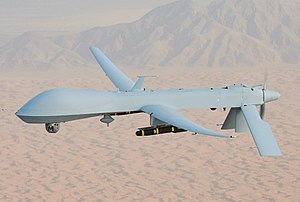
\includegraphics[width=0.6\linewidth]
    {Preliminaries/figures/Predator.jpg}
    \caption{General Atomics MQ-1 Predator. A \gls{RPA}. Source: \href{https://en.wikipedia.org/wiki/General_Atomics_MQ-1_Predator}{Wikipedia}}
    \label{fig:predator}
\end{figure}

%% Primeros UAV (drones autónomos). 
Later, with the development of technology, the first computers of sufficient size and computing power to run the software necessary to operate a \gls{UAV} autonomously and even to control aircraft with more complex and even unstable dynamics (gliders \cite{predator, BIGBLUE}, airships \cite{AURORA}, quadrotors \cite{quadrotorsreview, mesicopter, pounds, miniquadrotor}, multirotors \cite{fullyactuated}, flapping wings \cite{COLIBRI, GRIFFING, GRIFFIN2021}, etc.) appeared. Even though computational capacity was still insufficient for some applications, the development of \gls{UAV} systems was made possible by performing calculations on the ground. What was done was to run the critical and most important systems for autonomous flight on the on-board computer (controls, data acquisition, obstacle avoidance, etc.), and to run the more demanding calculations that are not necessary in real time on the ground computers \cite{OffBoard}.

\begin{figure}[htbp]
    \centering
    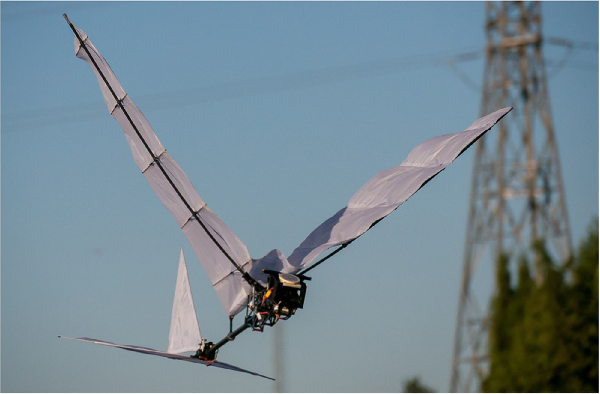
\includegraphics[width=0.6\linewidth]
    {Preliminaries/figures/GRIFFIN.png}
    \caption{GRIFFIN's flapping wing robot \cite{GRIFFIN2021}}
    \label{fig:griffin}
\end{figure}

%% Adquisición de datos (para ser autónomos necesitan recolectar datos del entorno)
For an aerial vehicle to operate autonomously, it is necessary to acquire data from the environment and process it in real time. A large number of different sensor configurations as well as numerous data acquisition and processing techniques can be found in the current literature \cite{SenseAndAvoid, aasen2018quantitative, miningSensors}.

%% Aplicaciones para UAV existentes (que necesitan de un piloto humano que supervise, no son cognitivos)
%% Equipos multi-UAV (con supervisión humana) [multiUAVclassification]
%% Explosión de la tecnología.
Once UAV technology reached sufficient capacity and autonomy, the first applications for both single \cite{nex2014uav, radoglou2020compilation, drummond2015uav} and multi-\gls{UAV} \cite{martinez2007multi, gu2018multiple, scherer2015autonomous} equipment began to appear. There is great interest in the latter, as they can be configured in different ways \cite{multiUAVclassification}, collect and process data in a distributed way, increasing the computational capacity of the equipment \cite{pascarella2015parallel, guo2021coded}, and generate global collective behaviour emerging from interactions between a large number of \glspl{UAV} that individually are relatively simple, known as swarming \cite{zhou2020uav, campion2018uav, chen2020sidr}. 

%% Esfuerzo para el desarrollo de aplicaciones sin presencia humana: capacidades cogitivas, entornos dinámicos. (Aerial co-workers)
Current applications often require human presence to carry out certain decisions, with the human pilot overseeing that everything runs smoothly and providing the cognitive capacity to analyse the generally dynamic environment and react to unforeseen situations \cite{sebbane2015smart, MITfullyAutonomous,kopeikin2012flight}. This is because providing a \gls{UAV} with sufficient cognitive capacity to operate fully autonomously in dynamic environments is a very complicated task and requires a great deal of processing power. In recent years, \gls{UAV} technology has evolved rapidly, benefiting from advances in computing and artificial intelligence. As processors are becoming more powerful, efficient and smaller, \glspl{UAV} are becoming more and more powerful without increasing their weight or compromising their autonomy. With the increase in the number of operations per second that \glspl{UAV} can perform, this opens up the possibility of using drones for previously unthinkable applications, applications that require a large amount of processing and usually have to be performed in real time \cite{CivilAplications, shakeri2019design}. At the same time, advances in artificial intelligence mean that the perception, analysis and sensory fusion capabilities of \glspl{UAV} are getting better and better. Advances in technology are breaking down one of the barriers preventing \gls{UAV} technology from achieving this level of autonomy, and with it, more and more research effort is being devoted to breaking down the other barrier, developing software that enables \glspl{UAV} to have cognitive capabilities.

%% Investigaciones recientes para aplicaciones 100% autónomas
% Aerial Co-workers
% Mencionar proyectos en los que está involucrada la universidad de sevilla
Mentioning some of the research that is currently being carried out, we can recall the well-known AERIAL-CORE European project\footnote{AERIAL-CORE European project homepage: \url{https://aerial-core.eu/}}, in which major European robotics teams are jointly participating with the aim of developing a fully autonomous robotic system with sufficient cognitive capabilities to work together with human operators in inspection and maintenance work on electrical networks \cite{cacace2021safe}. The PILOTING European project\footnote{PILOTING European project homepage: \url{https://piloting-project.eu/}} aims to develop a complete inspection platform that will provide its users with the information they need to draw up maintenance plans for structures \cite{benjumea2021localization}. HYFLIERS \footnote{HYFLIERS European project homepage: \url{https://www.oulu.fi/hyfliers/}} is a completed European project that focused on the inspection of long pipe arrays in hard-to-reach areas. This, unlike the previous two, is not fully autonomous, but needs a pilot to indicate the inspection points along the pipes, and to supervise the aerial robot while it operates \cite{suarez2020aerial}. It is also worth mentioning a recent \acrshort{NASA} (\acrlong{NASA}) achievement, which is no less than the first flight of an \gls{UAV} outside the Earth \cite{schroeder2020nasa, potter2020mars}. This is specifically the Martian helicopter called Ingenuity, whose mission was simply to take off, move around and land in the Martian atmosphere with the added difficulty that, due to the distance between the two planets, this had to be done completely autonomously.

% Related work: buscar artículos que tengan que ver con mi proyecto para poner en contexto lo que voy a aportar.
\section{Related work}
\label{sec:RelatedWork}
%%% Parrafo de introducción del trabajo relacionado con el mío: planificador de tareas cognitivo para  operaciones de inspección
According to the literature review conducted by Hazim Shakhatreh et al. in 2019 \cite{CivilAplications}, the market value of \glspl{UAV} for civil infrastructure inspection is expected to be more than \$45 billion, representing 45\% of the total \gls{UAV} market. The development of heterogeneous \gls{UAV} fleets and efficient algorithms for their communication and coordination is important to have multi-\gls{UAV} teams capable of carrying out a successful inspection and maintenance mission. If the inspection equipment is to be fully autonomous, so that it can be operated by personnel not specialized in the piloting of aerial vehicles, a module capable of reacting to any unforeseen event and modifying the planning in real time if necessary is required. This module, which could be called a task planner, is usually part of a larger software architecture in charge of fleet management and which tries to provide intelligence to the equipment. The task planner developed in this thesis consists of two distinct modules, the task planner itself and the behaviour manager.

\subsection{Task planning in multi-drone teams}
\label{subsec:TaskPlanning}
%% Hablar de las formas existentes que hay para abordar el problema del reparto de tareas en equivos multi-UAV.
There are numerous proposals for solving the task planning problem, each with its strengths and weaknesses. Given the lack of a rule of when one planner or another is better, Jiang et al. \cite{jiang2019task} compared the performance of the different planners in the literature. The conclusion they reached was that \gls{PDDL}-based planners are better on problems requiring long solutions, while \gls{ASP}-based planners are less susceptible to domain object augmentation. When complex reasoning is required, \gls{ASP}-based solutions can be considerably faster than \gls{PDDL}-based solutions. On the other hand, in \cite{canal2019probabilistic} they present a standardized integration of probabilistic planners in ROSPlan, which is a framework for task planning in the \gls{ROS}. By integrating \acrshort{RDDL} (\acrlong{RDDL}) into ROSPlan, they allow combining deterministic and probabilistic planning within the same system.

An example of probabilistic planning is presented in \cite{gao2018multi}, where they use an improved multi-objective particle swarm optimization algorithm to solve the task allocation problem for multiple \glspl{UAV}. The system consists of two phases with which they try to accelerate convergence and avoid the algorithm falling into local minimum. The results shown by this study reveal a good performance in solving this kind of problems. From a completely different approach, \cite{jolly2010intelligent} proposes an intelligent task planner focused on fuzzy neural networks. This system selects the best action from a set of possible actions. Time-constrained planning is also something that has been researched, e.g. \cite{nikou2016cooperative} incorporates time constraints into the planning of multi-agent systems. The proposed solution consists of two phases, first all execution times are pre-computed in a decentralized way and then the possible configurations are tested so that the collective execution time is guaranteed. Finally, mention can be made of \cite{ramchurn2015study}, where the final planning is done by humans, but they have a series of control interfaces and coordination algorithms that assist them in the decision-making process and compute the shortest path for each \gls{UAV} taking into account the priorities of the tasks and the type of \gls{UAV} required in each of them. The human commander can modify the plan or include constraints, such as assigning a task to a particular \gls{UAV} for example, and will have to review and accept the plan suggested by the algorithm once it is finished.

%% Poner en contexto lo que voy a aportar con mi TFM.
The task planner proposed in this work tries to group in the same system strong points such as robustness to failures, the capacity to react and replan online in case of any unforeseen event, the incorporation of restrictions and the consideration of factors such as the type of \gls{UAV}, the priorities of each task or the battery level of each equipment in an automatic way, without the need for human supervision.

\subsection{Drone behavior management}
\label{subsec:DroneBehaviorManagement}
In this work it has been called drone behaviour manager to what would commonly be controllers and safety modules executed at different times and levels. Once the aerial vehicle has concrete orders of what to do, in this case, once it has an assigned plan, it is time to execute the controls in charge of carrying out that plan. On the one hand, it will be necessary to execute some control in charge of supervising and ensuring the integrity of the airborne equipment. In \cite{monterrosa2016design} a \gls{FSM} is used in which one of the states is in charge of managing emergency situations, to which it transitions when another module detects and communicates the emergency condition. On the other hand, a high-level controller has to be executed in charge of calling the corresponding low-level controllers at any given moment. In this last study, they develop the complete flight control using \glspl{FSM} that transition from one state to another depending on the information provided by the sensors. The use of finite state machines is in fact the most common. In \cite{kugler2017autoland} for example, an automatic landing system programmed in this way is presented. Vitor de Araujo et al. \cite{de2014parallel} present a solution for the control of UAVs in search and rescue tasks based on a \gls{PHFSM} with which they claim to achieve many improvements with respect to other typical implementations.

%% (poner a lo mejor imagen de las FSM de \cite{de2014parallel})
The problem with this approach is that state machines are difficult to scale and reuse. Moreover, there comes a point where it becomes even difficult for a human to interpret. There is therefore a problem with further increasing the capabilities of \glspl{UAV} using state machines. As discussed in \cite{klockner2013behavior}, \glspl{BT} are an alternative that provide, among other advantages, scalability, modularity and readability, and could be used for \gls{UAV} mission management. \cite{ogren2012increasing} also emphasizes the advantages of using this type of system for \gls{UAV} control.

%% Poner en contexto lo que voy a aportar con mi TFM. Hablar de las FSM y de los BT
Although \glspl{BT} are already widespread in the videogame industry, there are still not many proposals that use them for the management of autonomous systems. The module in charge of controlling the behaviour of each of the \glspl{UAV} in this project has been developed using \glspl{BT}.

\section{Tools}
\label{sec:Tools}
% Estudio previo / Herramientas
This section discusses the most relevant software tools used in this project and briefly explains what role they have played in it.

\subsection{ROS}
\label{subsec:ROS}
The \acrlong{ROS} (\acrshort{ROS})\footnote{ROS homepage: \url{https://www.ros.org/}} is more of a framework than an operating system. It is a collection of tools, libraries and conventions that aim to facilitate the development of software for robots. The aim of this tool is to enable research teams from all over the world to collaborate with each other and to take advantage of each other's work. \gls{ROS} is present in most robotics projects today. In this project, it forms the basis on which everything else is programmed, as it allows the use of many other very useful tools developed by the community, such as those mentioned below.

\subsection{Gazebo}
\label{subsec:Gazebo}
This is a simulation tool usually used by the robotics community to accurately simulate and test their systems. In addition to being open-source, it allows the entire system to be tested, from the design of the robot itself to its programming. In this project, Gazebo has been used to test the developed software safely both in the development phases and in the final stages of testing and verification.

\subsection{Rviz}
\label{subsec:Rviz}
Rviz is a tool for visualizing information in 3D. It also allows to graphically represent the information received by a robotic system. It can be integrated with ROS applications, being very useful for debugging tasks. Rviz is used in this project to visualize the position of each of the UAVs as well as different details about the simulation for monitoring and debugging purposes.

\subsection{UAL}
\label{subsec:UAL}
As its name suggests, \gls{UAL}\footnote{UAL repository: \url{https://github.com/grvcTeam/grvc-ual}} is a software layer that simplifies the process of developing and testing high-level algorithms for aerial robots by standardizing and simplifying the interfaces with these robots. In addition, \gls{UAL} can work with both simulated and real platforms \cite{real_ijars20}. This software is also available in \gls{ROS} for free use in any robotics project. Although in this thesis a higher level software layer has been developed, which does not have to communicate directly with the autopilot of any of the aerial vehicles, it has been necessary to communicate with them in order to test the correct functioning of the task planning approach in simulation. Therefore, \gls{UAL} has been used in this project to programme at a low level the movement of the \glspl{UAV}, ignoring which autopilot they will incorporate in the future.

\subsection{Behaviour Trees}
\label{subsec:BehaviourTrees}
BehaviorTree.CPP\footnote{BehaviorTree.CPP repository: \url{https://github.com/BehaviorTree/BehaviorTree.CPP/}} is a C++ 14 library for creating behaviour trees. Its design features include flexibility, ease of use and speed. This library, among other things, allows the creation of asynchronous Actions, enables reactive behaviours that execute multiple Actions at the same time, permit to load trees at runtime and provides a type-safe and flexible mechanism to do Dataflow between Nodes of the Tree. This library has been chosen over others that fulfil the same function because of its documentation and support. Its function in this project has been the creation of \glspl{BT} for the programming of the drone behaviour manager in a modular, scalable and easily reusable way.

\subsection{Groot}
\label{subsec:Groot}
Groot\footnote{Groot repository: \url{https://github.com/BehaviorTree/Groot}} is a graphical editor to create \glspl{BT}. It is compliant with the library used in this project to create behavior trees, BehaviorTree.CPP. This graphic interface can be also used to monitor a running behavior tree. For programming \glspl{BT} in this project a simple XML file editor will be used, so Groot's role in this project will be to monitor the execution of the \glspl{BT} during testing.

\begin{figure}[htbp]
    \centering
    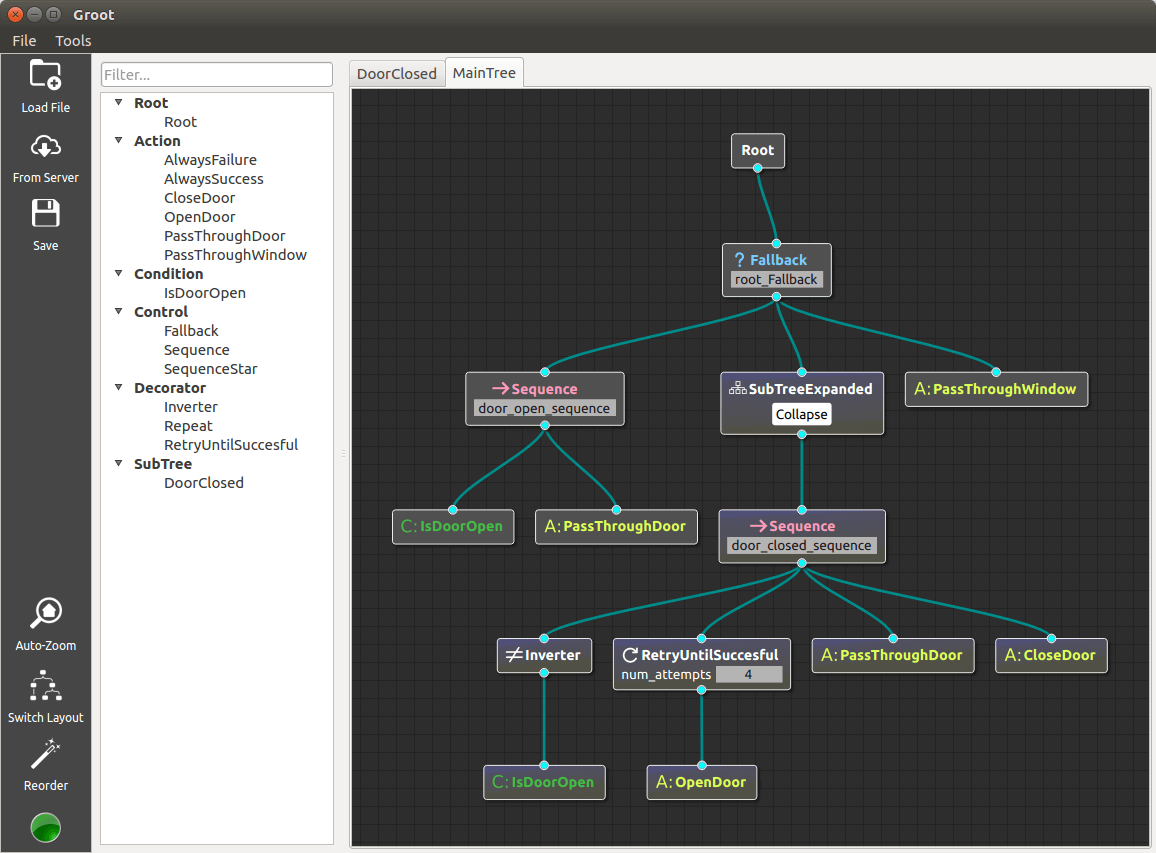
\includegraphics[width=1\linewidth]
    {Preliminaries/figures/groot.png}
    \caption{Groot graphical interface for editing behavior trees. Source: \href{https://github.com/BehaviorTree/Groot}{Github}}
    \label{fig:groot}
\end{figure}

\endinput
% 
%\chapter{Teoric Approach}
\label{ch:TeoricApproach}

% Estudio teórico
% Programas usados, software empleado, entorno de programación
% Metodología de trabajo
% Hablar de las diferentes formas existentes de abordar los dos problemas a solucionar:
%     Formas de afrontar el reparto de tareas
%     Formas de afrontar el control del comportamiento de los Agentes (BT, FSM)

\lettrine[lraise=-0.1, lines=2, loversize=0.2]{L}{o}rem itsum

%
%% Capi: En los capítulos 3 y 4 puedes coger texto del documento que tenemos hecho con Giuseppe, y del proyecto tuyo de tesis.
\chapter{Problem Formulation}
\label{ch:ProblemFormulation}
\lettrine[lraise=-0.1, lines=2, loversize=0.2]{A}{s} mentioned in Chapter \ref{ch:Introduction}, the context around which this cognitive task planner is being developed is the inspection and maintenance of electrical networks. Although one of the objectives is to build a task planner whose characteristics allow its easy reuse and adaptation for other applications, it is relevant to state the problem for which it is being originally prepared. 

As already mentioned, the AERIAL-CORE project aims to develop different technologies for the use of multi-\gls{UAV} system in inspection and maintenance tasks in high-voltage electrical installations. In particular, one of the technologies proposed is the use of \glspl{ACW}, i.e. small teams of cooperative \glspl{UAV} to safely support maintenance workers while working at height on power lines. These systems would have to interact with humans (see Figure \ref{fig:aerial_co_worker}) to inspect certain parts that are indicated to them, monitor worker safety during operation and deliver tools or other light equipment, in order to make the work more efficient and safer. In addition, to have a greater impact, the system would need to operate over extended periods of time, being able to autonomously deal with certain faults or recharges.

\begin{figure}[htbp]
    \centering
    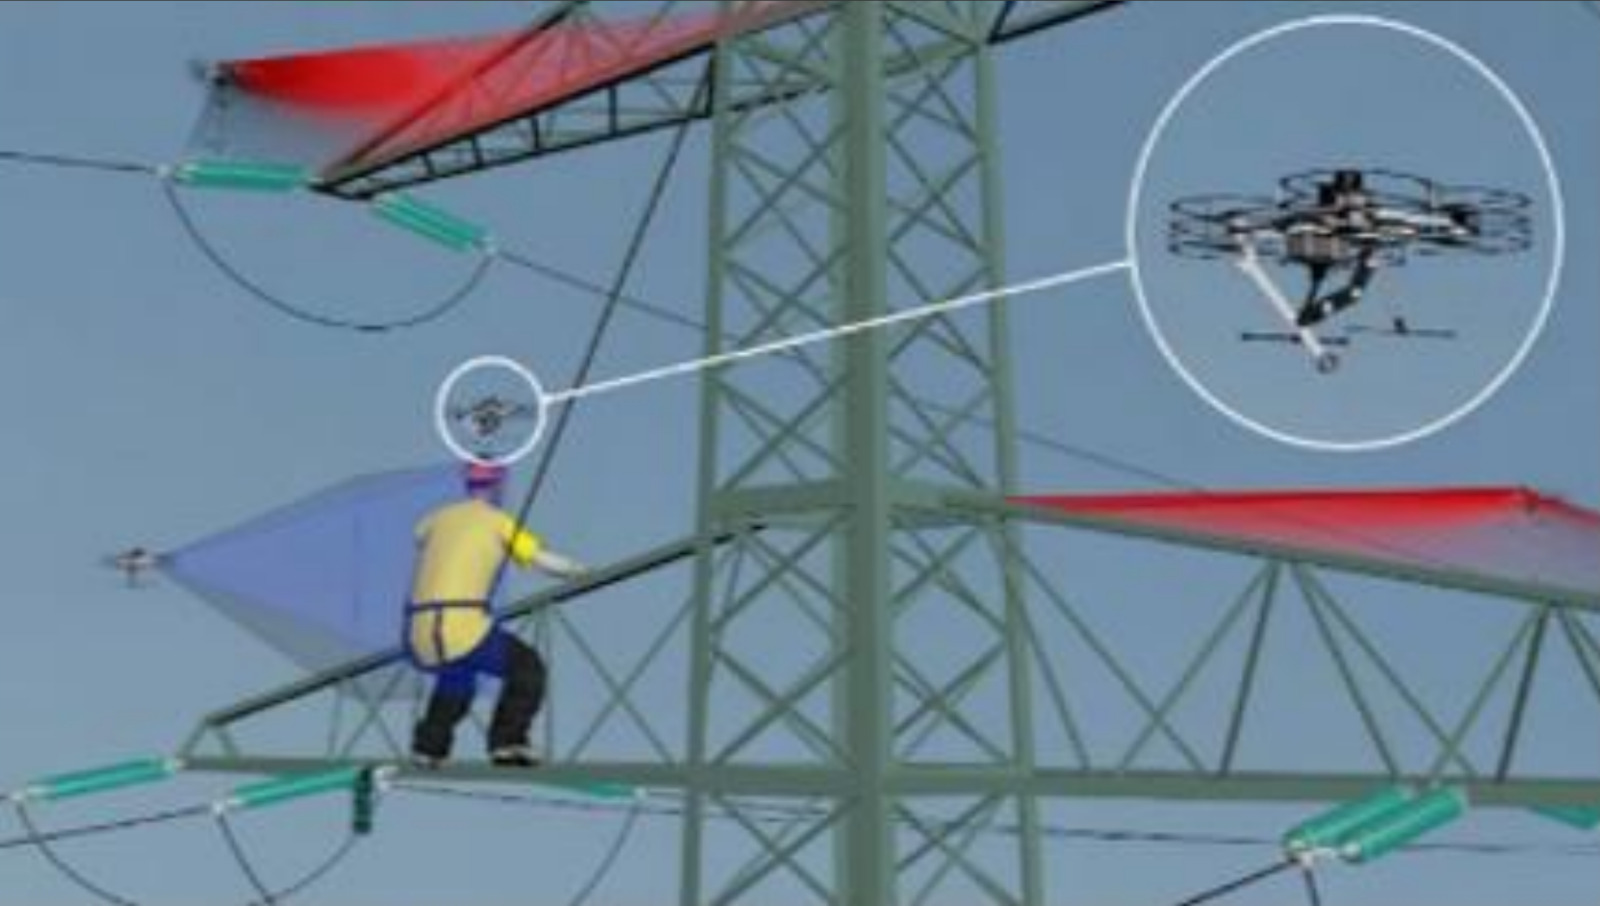
\includegraphics[width=.75\linewidth]
    {ProblemFormulation/figures/aerial_co_worker.jpeg}
    \caption{Multi-\gls{UAV} team supporting an operator. Source: \href{https://aerial-core.eu/}{Aerial-Core website}}
    \label{fig:aerial_co_worker}
\end{figure}

Three types of \glspl{ACW} are referred, each intended to provide different functionality: \textit{Inspection-ACW}, \textit{Safety-ACW}, and \textit{Physical-ACW}. The use case scenarios can be summarized as follows: 

\begin{itemize}
    \item \textit{Inspection}, where a fleet of \glspl{ACW} (i.e., \textit{Inspection-ACWs}) carries out a detailed investigation of power equipment autonomously, helping the human workers to acquire views of the power tower that are not easily accessible (see Figure \ref{fig:inspection_task});
    \item \textit{Safety}, where a formation of \glspl{ACW} (i.e., \textit{Safety-ACWs}) provides the supervising team with a view of the humans working on the power tower in order to monitor their status and to ensure their safety (see Figure \ref{fig:monitor_task});
    \item \textit{Physical}, where an \gls{ACW} (i.e., \textit{Physical-ACW}) physically interacts with the human worker and provides physical assistance to it, i.e., while in contact with the human it flies stably, reliably, and accomplishes the required physical task (e.g., handover of a tool) without becoming harmful for the human worker (see Figure \ref{fig:deliver_task}).
\end{itemize} 

Even if there is a specific type of \gls{ACW} for each of the tasks (inspection, monitoring and tool delivery), this does not mean that a \gls{UAV} can at any given time undertake a task for which it is not the best. It will therefore be the planner's task to take into account which \glspl{ACW} are best suited for each task, which are not but could perform it without problem, and which do not have the capacity to perform it at all. As a consequence, the number of ways in which the mission planning can be carried out multiplies, thus considerably increasing the difficulty of the problem that the task planner has to solve.

This mission planning problem with multiple \glspl{UAV} with battery constraints can be posed as an optimization problem, the solution of which indicates the most efficient way to allocate the different tasks and plan recharges. To react to possible failures, one of the most widespread options is to come up with dynamic methods that can replan in real time as certain events occur. Although there are many variants, most formulations for missions where multiple vehicles visit multiple locations to inspect or make deliveries give rise to NP-hard optimization problems and, therefore, the most widespread approach is to solve them using heuristic algorithms.

Planning methods based on uncertainties are appropriate for adding cognitive capabilities to a system that has to interact with humans in dynamic environments, as they allow optimizing plans by predicting the most likely intentions of humans and the outcomes of future actions. The main problem is their computational complexity, as the plan search space would grow exponentially with the number of \glspl{UAV} and with the future time horizon over which planning is to take place.

It is in this context and with these ideas in mind, the cognitive task planner in this thesis was developed. As this cognitive planner is a module part of a bigger software architecture to tackle the whole problem, the complete picture of that architecture is briefly introduced. Mainy, which information exchanges exist between the upper and lower layers of the software architecture, the interfaces by which this information travels, and the interactions between layers to activate low-level controllers. In the following section this information is presented by individually explaining the different tasks contemplated in the project. 

Additionally, a review will be made of other important considerations that the planner has to take into account, such as battery recharges, connection losses and task rescheduling; analyzing the different situations in which each of them can occur and their different causes. 

\section{Description of tasks}
\label{sec:DescriptionOfTasks}
As mentioned above, three different types of tasks are envisaged in the project. These tasks are requested at any time by human workers through gestures. There will be a higher level software layer that processes the information contained in the gestures so that the planner receives an asynchronous communication from the upper layer containing the specifications of a new task. At this point, it is the planner's job to process the new information together with the information it already had in order to elaborate and implement a new plan. The same planner is also in charge of calling the low-level controllers when necessary and ensuring the safety of the \glspl{UAV} and the fulfillment of the mission. Each task is explained in detail in the following sections.

\subsection{Inspection tasks}
\label{subsec:InspectionTasks}
This task can be performed by all three types of \glspl{ACW}. It is the second highest priority task, with the tool delivery task being the only one that exceeds it. It consists of carrying out a detailed inspection of the specified areas of the power equipment. The layer immediately above the task planner is responsible for passing it a list of \glspl{WP} that define the inspection task, and the planner is responsible for deciding how many \glspl{ACW} it recruits to execute the task, which of the available \glspl{ACW} it assigns it to, and which subset of the list of \glspl{WP} it assigns to each one. Once the planning is executed, the tasks of this type are transmitted to the lower level layers containing the subset of \glspl{WP} and the \glspl{ID} of the selected \glspl{UAV}.

All the aforementioned communications will be carried out asynchronously, as the creation of the task by the workers, which triggers the whole sequence of actions, is done in this way.

\begin{figure}[htbp]
    \centering
    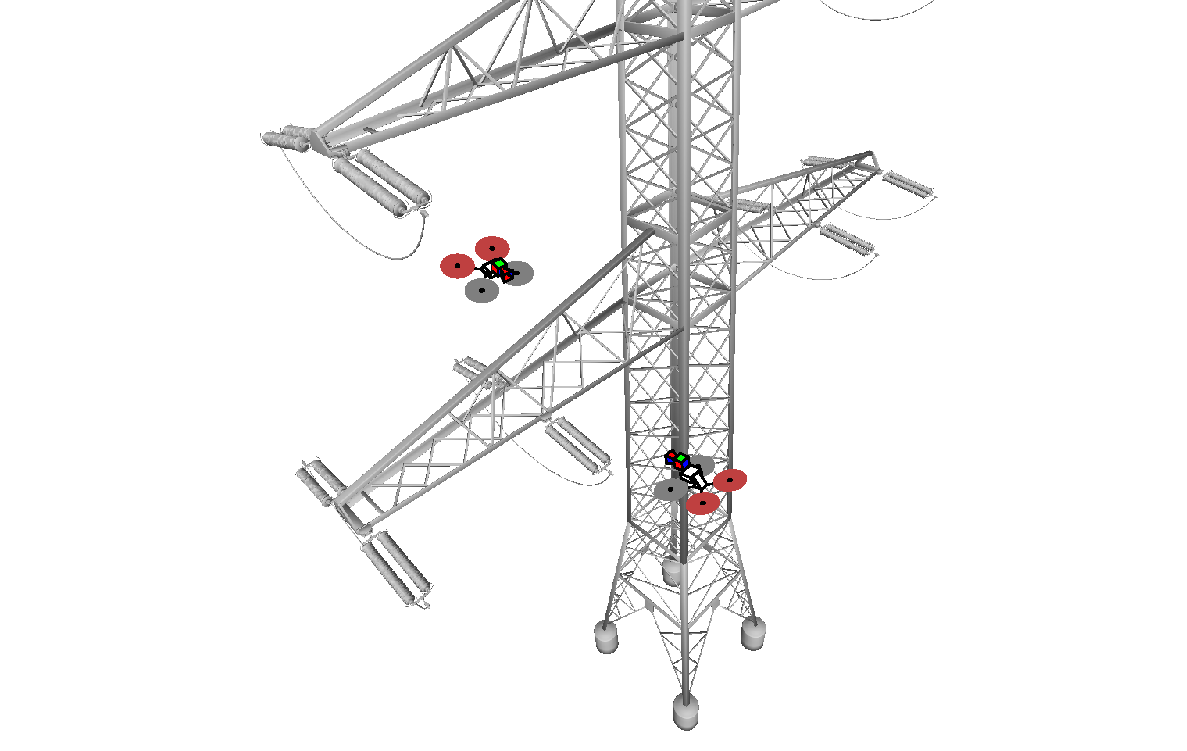
\includegraphics[width=.75\linewidth]
    {ProblemFormulation/figures/inspection_task.pdf}
    \caption{\textit{Inspection-ACW} carrying out an inspection task}
    \label{fig:inspection_task}
\end{figure}

\subsection{Monitoring tasks}
\label{subsec:MonitoringTasks}
This task can also be executed by all three types of \glspl{ACW}. It is the lowest priority task. Monitor worker's safety consists of providing the supervisory team with a view of the people working in the power tower to monitor their status and ensure their safety. The layer immediately above the task planner communicates this time the \gls{ID} of the worker to be monitored, the number of \glspl{UAV} desired and the distance they should keep from the worker. It is the task planner's responsibility to decide once again which of the available \glspl{ACW} to assign to this task and the formation they should maintain during the flight. Once the planning has been carried out, the tasks of this type are passed on to the lower level layers with both the original information and the information resulting from the planning.

The aforementioned communications will also be carried out asynchronously for the same reason. 

\begin{figure}[htbp]
    \centering
    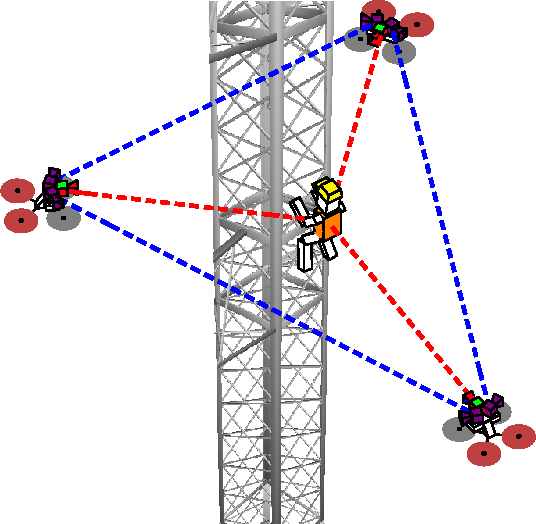
\includegraphics[width=0.5\linewidth]
    {ProblemFormulation/figures/monitor_task.pdf}
    \caption{\textit{Safety-ACW} carrying out a monitoring task}
    \label{fig:monitor_task}
\end{figure}

\subsection{Tool delivery tasks}
\label{subsec:ToolDeliveryTasks}
This task can be performed only by \textit{Physical-ACW} \glspl{UAV}, as special hardware is required to perform the physical interaction with the low-weight objects and the human. This is the highest priority task. Delivering a tool consists of picking up a tool and transporting it to the worker, with whom a physical interaction will take place through which the delivery of the tool will take place. Low-level controllers will have to be especially precise and careful not to hurt the worker. This time, the layer immediately above the task planner communicates the \gls{ID} of the worker to whom the tool is to be delivered and the \gls{ID} of the requested tool. Again, the task planner's mission is to decide to which of the available \glspl{ACW} assign this task. Once the planning is carried out, tasks of this type are passed on to the lower level layers with the same information as originally.

The aforementioned communications, once again, will be carried out asynchronously. 


\begin{figure}[htbp]
    \centering
    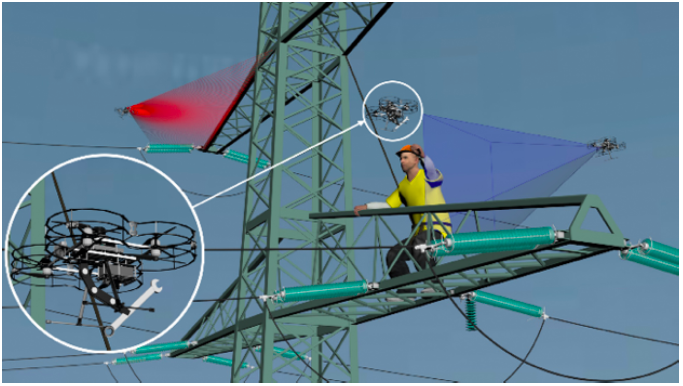
\includegraphics[width=0.7\linewidth]
    {ProblemFormulation/figures/deliver_task.png}
    \caption{\textit{Physical-ACW} carrying out a tool delivery task}
    \label{fig:deliver_task}
\end{figure}

\section{Battery recharges}
\label{sec:BatteryRecharges}
Given the current autonomy problem with \gls{UAV} technology, eventually each of the \glspl{ACW} involved in the mission will run out of battery power. The moment when the battery of each one will run out can be estimated from the mission planning itself, so the planner can take this into account when distributing the tasks so that the \gls{ACW} itself anticipates this event. Recharging does not necessarily have to take place when the \gls{UAV} is about to run out of battery, nor does it have to take place until the battery reaches its maximum, but both will be parameters to be taken into account during the mission planning and optimization process.

Besides, it is possible that the calculations may fail for some reason, and the battery may run out sooner than expected. It will therefore be necessary to periodically read the battery status and perform emergency recharging and replanning if necessary, reacting to unexpected faiulres. One possible scenario is that the aerial robot runs out of battery during a loss of connection. Since the planner is centralised at a ground station, there should also be a battery check and action module on board each aerial vehicle, and an emergency protocol in case this happens.

In the absence of specifications, it is assumed that battery recharging does not occur instantaneously (it is not a battery change), so reaching the desired battery level takes a certain amount of time that should be considered in the plan.

Also, the task planning algorithm has to be able to handle without blocking situations where all \glspl{ACW} are simultaneously without sufficient battery power and therefore there is no \gls{UAV} with which to execute a task immediately.

\section{Connection losses}
\label{sec:ConnectionLosses}
Another important consideration is the possible loss of connection between the centralised planner, where most of the cognitive capacity is concentrated, and one of the \glspl{ACW}. Since a loss of connection is an unforeseen event, it is most likely that the planner will recalculate the optimal task allocation once the \gls{UAV} fleet is updated, so that the tasks previously assigned to the disconnected \gls{ACW} will be executed on another one. This is a potentially dangerous situation because the disconnected \gls{UAV} could act autonomously according to its last plan and cause an accident with the rest of the agents that are still online.

It is therefore important: (i) to implement a system to detect disconnections from both sides of the communication, and (ii) to establish a common action protocol so that both modules know how the other is going to act, thus ensuring the integrity of all vehicles and the safety of the workers.

\section{Task replanning situations} % Unforeseen events
\label{sec:TaskReplanningSituations}
Once the mission is underway, any unforeseen event has the potential to completely change which the optimal plan is. Therefore, even if there is a possibility that the event will not affect the mission at all, it will always be necessary to execute a mission replanning in case of an unforeseen event.

The following is a list of the unforeseen events that have been contemplated in this work:

\begin{itemize}
    \item Arrival of a new task.
    \item Modification of a task's parameters.
    \item Connection of a new \gls{ACW}.
    \item Disconnection of an \gls{ACW}.
    \item Unplanned insufficient battery in one of the \glspl{ACW}.
    \item Battery drain faster than expected and therefore will not be enough for the current plan.
    \item An \gls{ACW} finishes recharging ahead of schedule.
    \item A task is successfully completed.
    \item A task is completed unsuccessfully.
\end{itemize}

Note that some of the events considered are not really unexpected. Successful completion of a task is what is desired, for example, so it should not imply a change of plans. However, this event is included in the list because it is a good moment to check if there is a better plan and to modify the current one if necessary. As the planner is pursuing the optimal plan, the result of the replanning will keep the previous plan unchanged if it is still optimal.
%
\chapter{Design of the proposed solution}
\label{ch:DesignOfTheProposedSolution}
\lettrine[lraise=-0.1, lines=2, loversize=0.2]{T}{his} section provides more details about the implementation of the solution to the problem: node diagram, pseudocode and inter-module communications. All the code is available online\footnote{Human aware collaboration planner source code: \url{https://github.com/grvcTeam/aerialcore_planning}}, and was developed under the Ubuntu 18.04 operating system and ROS Melodic.

The solution proposed for the problem formulated in the previous section (see section \ref{ch:ProblemFormulation}) follows a hierarchical approach, with a high-level planner in charge of activating different low-level controllers. The high-level planner detects the tasks required by the operators, and distributes them from the ground in a centralised way among the available \glspl{ACW}, planning the necessary reloads throughout the mission. In addition, this planner reacts in real time to possible failures by reassigning tasks. The low-level planners are on board each \gls{UAV} and are responsible for executing contingency plans for these failures while the central planner calculates and communicates the new plan. They will also be in charge of controlling the movement of the \glspl{ACW} to execute the different tasks assigned by the higher-level module (e.g. flying to a location to be inspected or to the position of an operator waiting for a tool). From now on, the low-level module on board each \gls{UAV} will be called the \emph{Agent Behaviour Manager}, and the centralised module on the ground will be called the \emph{High-Level Planner}. Together, these modules have cognitive capabilities enough to interact with humans efficiently. 

%%%%%% ATENTION %%%%%%%%%%%%%
% (\emph{No se si quitar esta última frase, este párrafo es adaptado del proyecto de tesis})

% Hasta ahora he explicado de qué módulos se compone la solución y que hacen pero no cómo lo hace.
% En "sec:NodeDiagram" comenzaremos explicando el diagrama de nodos (con la fig:NodeDiagram por delante) y luego describiremos de forma general el proceso que siguen los módulos
% En "sec:Centralized module:TaskPlanner" y "sec:Distributed module: behavior manager" se explicará cómo hacen lo que hacen 

\section{Node diagram}
\label{sec:NodeDiagram}
%% Informe de actividades: Node Diagram
As stated in chapter \ref{ch:Introduction}, the developed task planner is part of a software architecture consisting of different layers, being the main cognitive block the central layer, the \emph{high-level cognitive task planner}. Figure \ref{fig:NodeDiagram} shows a schematic of the software architecture from the perspective of the module implemented in this project, including the nodes that form it and their interfaces. The part of the diagram painted in grey would be the complete software architecture, including from the high-level module in charge of analyzing the gestures made by the operators to extract the tasks from them; to the low-level controllers in charge of executing those tasks. The software layer corresponding to this thesis, in charge of high-level decision-making, is marked in blue-green. It is composed of the \emph{High-Level Planner}, which is centralised and runs on a ground station, colored in orange; and the \emph{Agent Behaviour Manager}, distributed on board each \gls{ACW}, painted in lime.

\begin{figure}[ht]
    \hspace{-1cm}
	\scalebox{0.7}{
		\begin{tikzpicture}
    		% WP7 block
    		\node (WP7-Box) at (8.35,0) [fill=gray!15,rounded corners, draw=black!70, densely dotted, minimum height=5cm, minimum width=19.5cm]{}; 

			% Task planner box
    		\node (TaskPlannerBox) at ($(WP7-Box)+(0,0)$) [fill=teal!15,rounded corners, draw=black!70, densely dotted, minimum height=4.5cm, minimum width=14cm]{};
    		
    		% Gesture Recognition
    		\node (GestureRecognition) at (0,0) [text centered, fill=white, draw, rectangle, minimum width=1.5cm, text width=5.5em]{Gesture\\Recognition};
    		
    		\draw[-latex] ($(GestureRecognition) - (1.8,0)$) -- (GestureRecognition);
 
    		% High-Level Planner
    		\node (HighLevelPlannerBox) at ($(GestureRecognition) + (3.5,0.25)$) [fill=orange!15,rounded corners, draw=black!70, densely dotted, minimum height=2cm, minimum width=2.5cm]{}; 
    		\node (HighLevelPlanner) at ($(HighLevelPlannerBox) + (0,-0.25)$) [text centered, fill=white, draw, rectangle, minimum width=1.5cm, text width=5.5em]{High-Level\\Planner};
    		\node (Centralized) at ($(HighLevelPlanner) + (0,0.75)$) [text centered]{\small Centralized};
    		
    		\draw[-latex] (GestureRecognition.east) -- node[above]{Task} (HighLevelPlanner);
    		
    		%%%%%%%%%%%%%%%%%%%
    		% UAV 1
    		\node (UAV1) at ($(HighLevelPlanner) + (6.75,1.25)$) [fill=lime!20,rounded corners, draw=black!70, densely dotted, minimum height=1.7cm, minimum width=5cm]{}; 
    		\node (AgentBehaviourManager1) at ($(UAV1) + (0,-0.25)$) [fill=white, draw, rectangle, text centered, text width=12em]{Agent Behaviour Manager};
    		\node (UAV1-Text) at ($(AgentBehaviourManager1) + (0,0.75)$) [text centered]{\small On board ACW-$1$};	

    		\draw[fill=black] ($ (HighLevelPlanner.east) + (1.715,0) $) arc(-180:180:0.05);
    		\draw[-latex] (HighLevelPlanner.east) -- ($ (HighLevelPlanner.east) + (1.75,0) $) -- ($ (HighLevelPlanner.east) + (1.75,1) $) -- node[above]{Task} node[below]{List} (AgentBehaviourManager1.west);
    		\draw[-latex] ($ (HighLevelPlanner.east) + (1.75,0) $) -- node[above]{Feedback} (HighLevelPlanner.east);
    		
    		%%%%%%%%%%%%%%%%%%%
    		
    		% Dots
    		\node (Dots2) at ($(UAV1) + (0,-1.25)$) [text centered]{\dots};
    		
    		%%%%%%%%%%%%%%%%%%%
    		
    		% UAV N
    		\node (UAVN) at ($(HighLevelPlanner) + (6.75,-1.25)$) [fill=lime!20,rounded corners, draw=black!70, densely dotted, minimum height=1.7cm, minimum width=5cm]{}; 
    		\node (AgentBehaviourManagerN) at ($(UAVN) + (0,-0.25)$) [fill=white, draw, rectangle, text centered, text width=12em]{Agent Behaviour Manager};
    		\node (UAVN-Text) at ($(AgentBehaviourManagerN) + (0,0.75)$) [text centered]{\small On board ACW-$N$};	

    		\draw[-latex] (HighLevelPlanner.east) -- ($ (HighLevelPlanner.east) + (1.75,0) $) -- ($ (HighLevelPlanner.east) + (1.75,-1.5) $) -- node[above]{Task} node[below]{List} (AgentBehaviourManagerN.west);
    		
    		%%%%%%%%%%%%%%%%%%%
    		
    		% Lower-Level Controllers
    		\node (LowerLevelControllers) at ($(HighLevelPlanner) + (13.25,0)$) [text centered, fill=white, draw, rectangle, minimum width=1.5cm, text width=5.5em]{Lower-Level\\Controllers};
    		
    		\draw[-latex] (LowerLevelControllers.east) -- ($(LowerLevelControllers) + (1.8,0)$);
    		
    		\draw[fill=black] ($ (LowerLevelControllers.west) + (-1.535,0) $) arc(-180:180:0.05);
    		\draw[-latex] (AgentBehaviourManager1.east) -- ($ (LowerLevelControllers.west) + (-1.5,1) $) -- ($ (LowerLevelControllers.west) + (-1.5,0) $) --  node[above]{Task}
    	    node[below]{Params}	(LowerLevelControllers.west);
    		\draw[-latex] (LowerLevelControllers.west) -- ($ (LowerLevelControllers.west) + (-1.5,0) $) -- ($ (LowerLevelControllers.west) + (-1.5,1) $) -- node[above]{Task}
    	    node[below]{Result}	(AgentBehaviourManager1.east);
    		\draw[-latex] (AgentBehaviourManagerN.east) -- ($ (LowerLevelControllers.west) + (-1.5,-1.5) $) -- ($ (LowerLevelControllers.west) + (-1.5,0) $) -- (LowerLevelControllers.west);
    		\draw[-latex] (LowerLevelControllers.west) -- ($ (LowerLevelControllers.west) + (-1.5,0) $) -- ($ (LowerLevelControllers.west) + (-1.5,-1.5) $) -- 
    		node[above]{Task}
    		node[below]{Result} (AgentBehaviourManagerN.east);
    		
    		%%%%%%%%%%%%%%%%%%%%%
    		
    		\node (RealUAVs) at ($(WP7-Box.south) + (2,-1.25)$) [text centered, fill=white, draw, rectangle, minimum width=1.5cm, text width=6em]{ACWs\\autopilot};
    		\node (Humans) at ($(WP7-Box.south) + (-2,-1.25)$) [text centered, fill=white, draw, rectangle, minimum width=1.5cm, text width=6em]{Humans\\Tracker};
    		
    		\draw[-latex] (RealUAVs.north) -- node[right]{Pose, Battery, State} ($(WP7-Box.south) + (2,0)$);
    		\draw[-latex] ($(WP7-Box.south) + (2,0)$) -- (RealUAVs.north);
    		\draw[-latex] (Humans.north) -- node[left]{Pose} ($(WP7-Box.south) + (-2,0)$);
		
	    \end{tikzpicture}}
	\caption{Software architecture: nodes and interfaces. Node diagram from the high-level cognitive task planner perspective}
	\label{fig:NodeDiagram}
\end{figure}

In the software architecture scheme, although some communications are bidirectional, it can be seen that there is a main flow of information. Starting with the information arriving at the node \emph{Gesture Recognition}, this propagates to the last layer, where the \emph{Lower-Level Controllers} use the already processed information to command the \glspl{ACW}. The table \ref{tab:interfaces} shows the type of data that each of the nodes in the figure \ref{fig:NodeDiagram} receives as input and the type of data that each of them emits as output. Additionally, table \ref{tab:shareddata} explains what each one of the data mentioned in the previous table consists of.

% Description of the data interfaces for each software module
\begin{table}[ht]
    \centering
    \caption{Description of the data interfaces for each software module}
    \label{tab:interfaces}
    \small
    \begin{tabular}{|p{0.25\columnwidth}|p{0.25\columnwidth}|p{0.4\columnwidth}|}
      \hline
      \multicolumn{1}{|c}{\textbf{Module Name}} & \multicolumn{1}{|c|}{\textbf{Input Data}} & \multicolumn{1}{c|}{\textbf{Output Data}}\\ \hline \hline
      Gesture Recognition & Images & \textbf{Task, defined by:} Task ID, Task Type, Monitoring Distance, Monitoring Number, WP List, Tool ID (some task parameters will be ignored depending on Task Type) \\ \hline
      
      High-Level Planner & Task, Feedback (Task Result, BatteryEnough, \gls{BT} info), Humans' Pose, \glspl{ACW}' Pose, Battery and State, and Agent Beacon & Task List adding to each one its extra parameters result of the planning (Formation and/or List of \glspl{ACW}' IDs) and Planner Beacon \\\hline
      
      Agent Behaviour Manager & Task List, Low-Level's Result, Human Pose, \glspl{ACW} Pose, Battery and State & Params needed by Low-Level Controllers (depending on Task Type), Feedback (Task Result, BatteryEnough, \gls{BT} info) and Agent Beacon \\ \hline
      
      Low-Level Controllers & Params (depending on Task Type) & Result \\ \hline
      
      Humans Tracker &  & Pose \\ \hline
      
      \gls{ACW} autopilot & Low-Level orders & Pose, Battery and State \\ \hline
      
    \end{tabular}
\end{table}

% Description of data types
\begin{table}[htb]
    \centering
    \caption{Description of data types}
    \label{tab:shareddata}
    \small
    \begin{tabular}{|p{0.2\columnwidth}|p{0.15\columnwidth}|p{0.55\columnwidth}|}
      \hline
      \multicolumn{1}{|c}{\textbf{Data name}} & \multicolumn{1}{|c|}{\textbf{Data type}} & \multicolumn{1}{c|}{\textbf{Comment}} \\ \hline \hline
      
      Task ID & String & Unique identifier of each task \\ \hline
      
      Task Type & Integer & Task type indicator: m/M, i/I or d/D \\ \hline
      
      Human Target ID & String & Unique identifier of each human worker. The position of the human target and other needed info is supposed to be known and accessible via its ID. \\ \hline
      
      Monitoring Distance & Float & Distance from which the \gls{ACW} surveil the worker during a safety monitoring task \\ \hline
      
      Monitoring Number & Integer & Number of \glspl{ACW} that are required in formation for a certain safety monitoring task \\ \hline
      
      WP List & List of $3$ float tuples ($x$, $y$, and $z$) & List of waypoints to be inspected \\ \hline
      
      List of \glspl{ACW}' IDs & List of Strings & List of the unique identifiers of the \glspl{ACW} that have been selected for a task that requires multiple \glspl{ACW} \\ \hline
      
      Formation & Integer & Indicates which of the predefined types of formations should be used for monitoring (e.g., circle, triangle) \\ \hline
      
      Tool ID & String & Unique identifier of the tool to be delivered \\ \hline
      
      \gls{ACW}'s Pose & geometry\_msgs /PoseStamped & \gls{ACW}'s Position and orientation \\ \hline
      
      \gls{ACW}'s Battery & sensors\_msgs /BatteryState & Percentage of battery in the \gls{ACW} \\ \hline

	  Task Result & String, Boolean & First one is the task unique \gls{ID} and second one its result once it's finished \\ \hline
      
      Battery Enough & Boolean & Result of computing if an \gls{ACW} will have enough battery for its current task \\ \hline

	  \gls{BT} info & String list & Status of each \gls{BT}'s node in its last execution (Running, IDLE, SUCCESS or FAILURE) \\ \hline
      
      Agent Beacon & String, String & First one is the \gls{ACW}'s unique ID while the second one defines \gls{ACW}'s type (SafetyACW, InspectACW, or PhysicalACW). It is used as heartbeat and to detect new \glspl{ACW} in Planner \\ \hline

	  Planner Beacon & Time & ROS::Time message containing the time when the beacon was sended. It is used to check the status of the connection from Agent's side. \\ \hline
      
      Lower-Level's Result & Boolean & Result of the Lower-Level Controllers once they have finished after being called \\ \hline
      
    \end{tabular}
\end{table}

The first node is constantly checking the images captured by the \glspl{UAV} for a gesture that is indicating a new task or the modification of an existing task. When this occurs, it asynchronously emits a task, which will be picked up by the centralised planner. As shown in the table \ref{tab:interfaces}, this communication includes the unique \gls{ID} that differentiates this task from the others, the type of task and the parameters that define it.

On the other hand, the \emph{High-Level Planner}, when it receives this information, proceeds to re-evaluate the optimal plan taking into account the task received, the information it receives from the \emph{\glspl{ACW}' autopilot}, and the position of the operators, which is periodically published by the \emph{Human Tracker}. The aforementioned data set constitutes the input data for the \emph{High-Level Planner} together with the feedback coming from each \emph{Agent Behaviour Manager}. Its output data being a list of tasks for each gls{ACW}.

On board each \gls{ACW} is the \emph{Agent Behaviour Manager}. This node is in charge of collecting the corresponding task list provided by the centralised planner. With this input information and the information coming from the \emph{Human Tracker} and the \emph{\gls{ACW}'s autopilot}, this module is in charge of calling the \emph{Lower-Level Controllers} to carry out the execution of the assigned plan. The information emitted by the \emph{\gls{ACW}'s autopilot} is also used to check that everything is working correctly and to execute the security protocols in case they are necessary. If this happens, the corresponding communication would be issued back to the \emph{High-Level Planner} node in order to calculate a new plan. This node also receives the \emph{Lower-Level Controllers}' result after calling each of them, and publish back to the \emph{High-Level Planner} some feedback.

In addition to these communications, the nodes \emph{High-Level Planner} and \emph{Agent Behaviour Manager} periodically exchange beacons that are used to detect both the connection of a new \gls{ACW} and its disconnection in case of failure. Finally, there is an asynchronous communication that is broadcast to all nodes indicating the end of the mission when this happens.

Finally, it is worth mentioning that the \emph{Gesture Recognition} node does not have a communication aimed at modifying parameters of a task already contemplated within the \emph{High-Level Planner}. However, this is possible because tasks have a unique identifier. Once a task has been delivered to the \emph{High-Level Planner}, in order to change any of its parameters, the \emph{Gesture Recognition} node just has to submit the task again, keeping the same task \gls{ID} and updating only the desired parameters. Thus, the \emph{High-Level Planner} would overwrite it and allocate it again with the new parameters.

\section{Centralized module: High-Level Planner}
\label{sec:Centralized module:TaskPlanner}
%% Protocolo de desconexión
%% Protocolo de pérdida de batería
%% Que ocurre cuando una tarea termina
%% Replanificaciones de tareas: restricciones a la hora de planificar o replanificar

As mentioned above, the \emph{High-Level Planner} is a centralised module running on a ground station and constitutes the main cognitive block of the software architecture of which this project is a part. Its purpose is to plan the mission in an optimal way, i.e., to distribute the pending tasks among the available \glspl{ACW} by specifying the order in which they are executed and taking into account the time it takes to complete each one, the type of each \glspl{UAV}, the distance each one will have to travel, the battery they have available, the task each one was executing, the priority of each task, the battery consumed by each task, the recharges that will be needed and when it is best to carry out the recharges.

%% Explicación y Pseudocódigo general de como se inicializa el nodo planner, el bucle while(ros::ok) y como se cierra cuando mission_over. Incluir escucha a imprevistos.
The general pseudocode for this node from launch to termination is contained in the code \ref{ps:GeneralPlanner}.

\begin{lstlisting}[caption={General operation of \emph{High-Level Planner}'s code}, breaklines=true, label=ps:GeneralPlanner]
	1. Read from a ros::param the address of the configuration file.
	2. Read from the configuration file all necessary information.
	3. Configure ROS communications (Publishers, Subscribers and ActionServers).
	4. Set the loop rate.
	5. Main "while" loop. While ros::ok() and not mission over do:
		5.1. Check the timeout of the Agents' beacons.
		5.2. Publish a new Planner beacon.
		5.3. Check for pending incoming communications (ros::spinOnce).
		5.4. Sleep the remaining time to send the next beacon.
	6. Wait until all UAVs have finished and disconnected. While there is any agent connected do:
		6.1. Check the timeout of the Agents' beacons.
		6.2. Check for pending incoming communications (ros::spinOnce).
		6.3. Sleep for a while.
\end{lstlisting}

%% Decir que todo funciona con callbacks y explicarlos. (batteryEnoughCB, taskResultCB, positionCallback, batteryCallback)(incomingTask, beaconCallback, missionOverCallback)
Since the environment in which the \glspl{UAV} operates is dynamic, this module has been programmed in such a way that it can react to unforeseen events and recalculate the optimal plan. As can be deduced from the \ref{ps:GeneralPlanner} pseudocode, everything works through callback functions. Every time a communication arrives from another node, a response is triggered on that node. The information contained in the message is analyzed and it is decided whether a replanning is necessary or not. The situations in which a replanning has been deemed necessary are listed in section \ref{sec:TaskReplanningSituations}. The communications summarized in the tables \ref{tab:interfaces} and \ref{tab:shareddata} and in the figure \ref{fig:NodeDiagram} are sufficient to detect these unforeseen events and to be able to respond to them in the best possible way.

\begin{lstlisting}[caption={Task callback pseudocode}, breaklines=true, label=ps:IncomingTask]
	1. Check if the task already exists and delete it in order to create it with the new parameters.
	2. Read the type of task and the parameters that apply to it.
	3. Add the new task to the pending task list.
	4. Perform a task planning.
\end{lstlisting}

Firstly, there is the callback that is executed when the node \emph{Gesture Recognition} sends a task, which always ends up calling the function in charge of calculating the optimal plan (see code \ref{ps:IncomingTask}); the mission over callback, whose only action is to change the value of a variable so that the node exits the main while loop; and finally the agent's beacon callback, which is executed every time a \gls{UAV} beacon is received and whose pseudocode is the code \ref{ps:AgentBeaconCallback}.

\begin{lstlisting}[caption={Agent's beacon callback}, breaklines=true, label=ps:AgentBeaconCallback]
	1. Read the information contained in the beacon.
	2. If it is a connection of a new UAV:
		2.1. Register it in the database.
		2.2. Perform a task planning.
	3. Else, if it is the heartbeat of an already known UAV:
		3.1. Reset the timeout timer.
\end{lstlisting}

The action carried out by the agent's beacon callback varies depending on whether it is the beacon of a new \gls{UAV} or the heartbeat of a known \gls{UAV}. For each agent there will be an object in the database that will contain another series of callbacks that will be in charge of receiving the messages coming from the \glspl{ACW} and respond accordingly.

\begin{lstlisting}[caption={Callback that runs when an \emph{Agent Behaviour Manager} sends battery feedback}, breaklines=true, label=ps:batteryEnoughCB]
	1. Update the value of the internal flag associated with the battery.
	2. Perform a task planning.
\end{lstlisting}

The \emph{Agent Behaviour Manager} node only sends communications messages indicating the battery status when it is due to an unplanned event. This event can be either an early battery depletion or a faster than expected recharge. In both cases, the callback function whose pseudocode is the code \ref{ps:batteryEnoughCB} consequently updates the value of an internal variable used during planning, and recalculates the optimal plan.

The other possible communication coming from a node of type \emph{Agent Behaviour Manager} with the ability to trigger a reaction in the planner is due to the termination of a task. When a task finishes successfully, it is simply removed from the list of pending tasks. In addition, this moment is used to re-evaluate the optimal plan. It is expected that the mission is still within the optimal plan, so in that case the planning result should be the same as the plan that was already being executed. If, on the other hand, conditions have changed since the last planning and a better plan now exists, it is at this point that the plan is updated. On the other hand, if the task ends with a failure, the callback action will depend on the causes of the failure (note that the interruption of a task will result in a failure). If the interruption is due to the \gls{UAV} battery, it may be planned, in which case no action is required, or it may be unexpected, in which case the corresponding actions are taken by the battery callback. Once it has been verified that the task has not finished due to the battery, a check is made to see if the task was at the beginning of the queue. If so, a failure has indeed occurred, so the operators are warned, the task is removed from the list and a replanning is executed. Otherwise the task in question would have been moved from the top of the queue due to a change of plans and therefore no action would have to be taken either. The pseudocode corresponding to what has just been explained is in code \ref{ps:taskResultCB}.

\begin{lstlisting}[caption={Callback that runs when an \emph{Agent Behaviour Manager} sends a task result}, breaklines=true, label=ps:taskResultCB]
	1. Read the information contained in the task result.
	2. If the task result is SUCCESS:
		2.1. Delete it from the pending tasks list.
		2.2. Perform a task planning.
	3. Else, if the task result is FAILURE:
		3.1. If the task has been halted because of not having battery enough:
			3.1.1. Return.
		3.2. Else, if the task is on the front of that ACW's task queue:
			3.2.1. Notify operators that a task has failed and is going to be deleted.
			3.2.2. Delete task from the pending tasks list.
			3.2.3. Perform a task planning.
		3.3. Else:
			3.3.1. Return.
\end{lstlisting}

The other two communications received by the \emph{High-Level Planner} from the \glspl{ACW} are sensor readings corresponding to the \glspl{UAV}' position and battery percentage. In both cases the only action of the corresponding callback is to update the information with the new values.

The last function that remains to be explained of those that can potentially request a replanning of the mission is the one in charge of checking the timeout of the agents' beacons. As shown in the code \ref{ps:GeneralPlanner}, this function is not a callback like the previous ones, instead it is executed periodically in the main while loop. Its operation is shown in the code \ref{ps:checkBeaconsTimeout}. Simply, for each agent connected, it checks that the timeout amount of time has not elapsed since its last beacon was received. If a timeout has occurred, that \gls{ACW} is considered disconnected and is removed from the centralised node data. If, after checking all the agents, the number of connected \glspl{UAV} has decreased, i.e. if any of the previously connected \glspl{UAV} has disconnected, a mission replanning is executed.

% Pseudocódigo de checkBeaconsTimeout
\begin{lstlisting}[caption={Beacons' timeout check function}, breaklines=true, label=ps:checkBeaconsTimeout]
	1. For each agent connected:
		1.1. If the elapsed time since the last beacon is grater than the timeout time:
			1.1.1. Add that agent's ID to the list of disconnected agents.
	2. While the list of disconnected agents is not empty:
		2.1. Take first ID from the list.
		2.2. Erase from the node's data all information related to that ID.
	3. If any agent has been disconnected:
		3.1. Perform a task planning.
\end{lstlisting}

%% Explicar como se realiza la planificación y poner psudocódigo de cómo se lleva a cabo. Explicar también como se calcula el coste.
The pseudocode that is executed when one of these functions deems it necessary to perform a new task planning is summarized in the code \ref{ps:performTaskAllocation}. It is important to remember that some tasks have a higher priority than others, and this depends only on the type of task. To simplify the process, it has been decided to allocate the tasks in order of arrival, assuming that between two tasks of the same type, the one that arrived first will be more urgent, and therefore will be given higher priority. Therefore, when a new task is received, it is stored both in the \emph{std::map} that contains all the pending tasks to facilitate the access to the information, and in the \emph{std::vector} of its task type, where the order of arrival is maintained. What this simplification allows is to assign tasks one at a time. By having a prioritized list of tasks and assuming that no task can be assigned before a task with a higher priority, the mission planning problem is reduced to calculating the cost of each task individually for each \gls{UAV} with the ability to execute it and assign it to the one with the lowest cost. For monitoring-type tasks, the selection of the required number of agents is strictly cost-based. The \emph{N} agents that cost the least to execute the task are selected. The same is a little more complex for the tasks of type inspect, where the number of agents to select is a parameter to be defined by the planner itself. This value is first set according to the number of points to be inspected. Up to three points, a single \gls{ACW} is selected; up to six points, two are selected; and from seven points onwards, three agents are selected, this being the maximum number imposed by the low-level controller. Moreover, as the low-level controller in charge of this task works, all the \glspl{ACW} selected for this task are required to start executing it simultaneously, so a second approximation of this number is made according to the number of idle \glspl{UAV}. Thus, if they are assigned this as the first task, they will start executing it simultaneously. Academically, this simplification seems to deviate from the optimal solution, but it must be remembered that this work is part of a software architecture that will operate in real situations. In such situations, it is not expected that there will be a large number of \glspl{UAV} connected simultaneously, nor a long list of pending tasks. In such a simple scenario, it makes sense to make this simplification without deviating too much from the optimal solution. Finally, the number of agents to be selected will be the smaller of the two above, being equal to one when there is no \gls{UAV} idle and zero in case there is no \gls{ACW} with enough battery. In the latter case, the task would be assigned after recharging. Once the number of agents to be selected has been defined, the agents that have the least cost to execute the task are selected from among those that meet the conditions described. Having selected the \gls{ACW} that will carry out the task, all that remains is to distribute among them the \glspl{WP} to be inspected. Although the algorithm in charge of performing the optimal distribution is in the low-level controller of this task, as the rest of the modules that make up the software architecture are not yet available, it has been necessary to program a distribution algorithm in order to be able to carry out the experiments. More details on this will be given in section \ref{sec:LowerAndUpperLevelModulesFaker}.

% Explicar como se calcula el coste.
The cost for each \gls{UAV} is calculated as the weighted sum of three different types of costs. A first cost assesses the type of \gls{ACW} and penalizes the assignment of tasks to those \glspl{UAV} designed for another type. It penalizes especially the assignment of lower priority tasks to agents designed to perform higher priority tasks. The second cost evaluates the total distance the \gls{UAV} will have to travel from where it is at the beginning of the task to where it is at the end of the task. This cost is an approximation of the expected battery consumption, although it does not take into account intermediate travel and hoovering times during the mission. The last cost penalizes the interruption of the task that was being executed according to the previous plan and rewards the assignment of the same task. This cost is intended to ensure that a task is preferentially assigned to an idle \gls{UAV}, to an \gls{UAV} that is executing a lower priority task, or even to an \gls{UAV} of a different type, rather than interrupting a task unnecessarily just because that \gls{ACW} has to travel a shorter distance, for example.

\begin{lstlisting}[caption={Simplified task planning function's pseudocode}, breaklines=true, label=ps:performTaskAllocation]
	1. If there is any agent connected:
		1.1. For each agent connected:
			1.1.1. Make a copy of the current task queue.
			1.1.2. Empty the task queue.
		1.2. For each Tool Delivery task:
			1.2.1. Compute the cost of the task for each PhysicalACW that has battery enough.
			1.2.2. Assign the task to the agent for who the task cost the least (from those who has battery enough).
			1.2.3. Add the task to that agent's task queue.
		1.3. For each Inspection task:
			1.3.1. Extract from the task parameters the list of WP to inspect.
			1.3.2. For each ACW(any type) tha has battery enough:
				1.3.2.1. Compute the cost of the task for that ACW. 
				1.3.2.2. Check if that ACW is still idle.
			1.3.3. Calculate the number of agents to select for the task based on the number of WP and the number of idle agents.
			1.3.4. If no agent has battery enough, continue.
			1.3.5. Else, if the number of agents to select is equal to zero, assign the task to the agent that cost the least.
			1.3.6. Else, select the calculated number of agents for whom the task costs the least.
			1.3.7. Divide the WP to inspect among the selected agents.
			1.3.8. For each selected agent:
				1.3.8.1. Set the remaining task parameters (List of selected ACWs' IDs and divided WP list).
				1.3.8.2. Add the task to the agent's task queue.
		1.4. For each Monitoring task:
			1.4.1. Compute the cost of the task for each ACW (any type) that has battery enough.
			1.4.2. If required number of ACWs for the task is zero:
				1.4.2.1. Warn operators that this parameter can not be zero.
				1.4.2.2. Delete task from pending tasks.
			1.4.3. Else, select the requested number of agents for whom the task costs the least.
			1.4.4. Set the remaining task parameter (List of selected ACWs' IDs)
			1.4.4. Add the task to each selected agent's task queue.
		1.5. For each ACW connected, send the new task queue to its Agent Behavior Manager.
	2. Else:
		2.1. Warn operators that any agent is connected.
\end{lstlisting}

Once the calculation of the mission plan has been completed, the new task queues are sent to the corresponding distributed modules. Each \emph{Agent Behaviour Manager} will react to this communication and will take care of executing the newly assigned plan. In the meantime, the \emph{High-Level Planner} node returns to the main while loop to continue waiting until an event that triggers a replanning occurs again.

\section{Distributed module: Agent Behavior Manager}
\label{sec:Distributed module: behavior manager}
%% Explicar qué es una drone behavior manager y cual es su función.
This node is in charge of executing the plan assigned by the \emph{High-Level Planner}, of checking the security of the equipment at all times, of detecting unforeseen events and of communicating them to the centralised node so that it can make a change of plans if it deems it necessary. The \emph{Agent Behavior Manager} will communicate with the low-level controllers, handing over control when necessary to complete the assigned plan.

%% Estructura general del nodo (pseudocodigo). Explicar que se ha hecho con árboles de comportamiento en paralelo a algunos procesos de ros
The general structure of this node is quite similar to that of the central node. The pseudocode is summarized in the code \ref{ps:GeneralAgent}. Upon initialization, the \emph{Agent Behaviour Manager} prepares the necessary information to start its operation, configures the necessary communications, declares and initializes the behaviour tree and, once the \gls{UAV} it controls has finished initializing, starts sending beacons to the central node to inform it of its joining the mission. Once the code finishes initializing and reaches the main while loop, the activity of the \emph{Agent Behaviour Manager} concentrates on the execution of callbacks in response to incoming messages, as in the \emph{High-Level Planner}, and on the execution of the behaviour tree, which directs and supervises the \gls{UAV} movement.

\begin{lstlisting}[caption={General operation of \emph{Agent Behaviour Manager}'s code}, breaklines=true, label=ps:GeneralAgent]
	1. Read from a ros::param the beacon's content (ACW's ID and type).
	2. Read from a ros::param the address of the configuration file.
	3. Read from the configuration file all necessary information.
	4. Configure ROS communications (Publishers, Subscribers and ActionServers).
	5. Set the loop rate.
	6. Declare the behaviour tree.
	7. Initialize each BT node.
	8. Start BT loggers to to facilitate debugging and monitoring of the node's performance.
	9. Wait until the ACW fully initializes.
	10. Main "while" loop. While ros::ok() and BT status is running:
		10.1. If a timeout of Planner's beacons has not ocurred:
			10.1.1. Publish a new Agent beacon.
		10.2. Check if battery is enough for the current task.
		10.3. Check for pending incoming communications (ros::spinOnce).
		10.4. Sleep the remaining time to send the next beacon.
\end{lstlisting}

%% Explicar lo que es un árbol de comportamiento y compararlo con una máquina de estados.
The \glspl{BT} are who governs the \glspl{ACW} to perform each of the assigned tasks. Each \gls{BT} monitors its \gls{ACW}'s battery and task status and reacts to any possible failure or unexpected event, requesting a new re-planning to the \emph{High-Level Planner} in case of need. BT can be defined as an improved \gls{FSM}. They are a more advanced mechanism to implement behaviors, especially because of their advantages in terms of scalability, modularity, readability and reusability, facilitating the creation of more complex behaviours with less effort.

%% Informe de actividades: Diseño del árbol de comportamiento.
Despite this, the process of designing a state machine is nothing like the process of designing a behaviour tree. Designing behaviour trees without ever having done it before is not a trivial task. Moreover, there will be more than one valid implementation to achieve the same behaviour, which makes it more complicated to design this type of solution when you do not yet have enough intuition to know which one is better. Taking advantage of the fact that the use of \gls{BT} is widespread in the videogame industry, information about them was gathered and studied to try to develop enough knowledge and intuition to design from scratch a \gls{BT} that meets the needs of the mission. The examples found in \cite{BT-CPP-doc, colledanchise2018behavior, BT-AI} were very useful.

Before proceeding with the explanation of the designed BT, the types of nodes that can be found in the selected C++ library and the functioning of each of them will be briefly discussed.

%% Informe de actividades: Tipos de nodos de BT
\begin{figure}[htbp]
    \centering
    \subfloat[]{%Fallback
		\label{subfig:Fallback}
        \begin{tikzpicture}
			\node (MainTree) at (0,0) [text centered, fill=white, draw, rectangle, minimum width=0.5cm, text width=0.5em]{\textbf{?}};
		\end{tikzpicture}}
    \hfill
    \subfloat[]{%Sequence
		\label{subfig:Sequence}
        \begin{tikzpicture}
			\node (MainTree) at (0,0) [text centered, fill=white, draw, rectangle, minimum width=1.5cm, text width=1.5em]{$\longrightarrow$};
		\end{tikzpicture}}
	\hfill
    \subfloat[]{%Reactive
		\label{subfig:Reactive}
        \begin{tikzpicture}
			\node (MainTree) at (0,0) [text centered, fill=magenta!5, draw=magenta, rectangle, minimum width=2cm, minimum height=0.75cm, text width=2em]{};
		\end{tikzpicture}}
    \hfill
    \subfloat[]{%Common
		\label{subfig:Common}
        \begin{tikzpicture}
			\node (MainTree) at (0,0) [text centered, fill=white, draw, rectangle, minimum width=2cm, minimum height=0.75cm, text width=2em]{};
		\end{tikzpicture}}
    \hfill
    \subfloat[]{%Decorator
		\label{subfig:Decorator}
        \begin{tikzpicture}
			\node (MainTree) at (0,0) [text centered, fill=orange!5, draw=orange, rectangle, minimum width=2cm, minimum height=0.75cm, text width=2em]{};
		\end{tikzpicture}}
    \hfill
    \subfloat[]{%Action
		\label{subfig:Action}
		\begin{tikzpicture}
			\node (MainTree) at (0,0) [text centered, fill=blue!5, draw=blue, rectangle, minimum width=2cm, minimum height=0.75cm, text width=2em]{};
		\end{tikzpicture}}
		\hfill
    \subfloat[]{%Condition
		\label{subfig:Condition}
        \begin{tikzpicture}
			\node (MainTree) at (0,0) [text centered, fill=blue!5, draw=blue, ellipse, minimum width=2cm, minimum height=0.75cm, text width=2em]{};
		\end{tikzpicture}}
    \caption{Different types of nodes that can be present in an \gls{BT}}
    \label{fig:CounterRunImagenes}
\end{figure}

%% Del WP7_Scenarios: Funcionamientos de los BT (va con la imagen anterior)
 Behaviour Trees are made up of \emph{Control} nodes, \emph{Decorator} nodes, and \emph{Leaf} nodes. \emph{Control} nodes could be either \emph{Fallback} nodes, represented with a question mark (see subfigure \ref{subfig:Fallback}), which try success calling one by one each of their children; or \emph{Sequence} nodes, represented with an arrow (see subfigure \ref{subfig:Sequence}), which call their children in order if the previous one have succeded. \emph{Fallback} nodes return \emph{SUCCESS} if one of its children does it, \emph{FAILURE} if none of them return \emph{SUCCESS}, and \emph{RUNNING} if one of its children returns \emph{RUNNING}. On the other hand, \emph{Sequence} nodes return \emph{SUCCESS} when all children have been called in order and have returned \emph{SUCCESS}. If any of them returns \emph{FAILURE}, the sequence is broken and the \emph{Sequence} node returns \emph{FAILURE} too. When a child returns \emph{RUNNING}, \emph{Sequence} node does it too. \emph{Control} nodes are represented in a black rectangular box when they are the standard ones (see subfigure \ref{subfig:Common}), but they could also be \emph{Reactive} control nodes, represented by a magenta box (see subfigure \ref{subfig:Reactive}), which means that its already called children will be called again in the next iteration. This is very useful for generating behaviours where an action is constantly reattempted, or where it is necessary to check that the necessary conditions are still met. A \emph{Child} node could be another \emph{Control} node, a \emph{Decorator} node, a \emph{Leaf} node or a whole sub-tree. A \emph{Decorator} node, represented in an orange box (see subfigure \ref{subfig:Decorator}), can only have one child (of any type) and its function is programmable (e.g., modifying its child result or retrying calling its child a number of times). \emph{Leaf} nodes, represented in blue, could be \emph{Condition} nodes, represented in a blue elliptical shaped box (see subfigure \ref{subfig:Condition}), that check a condition and return either \emph{SUCCESS} or \emph{FAILURE}; or \emph{Action} nodes, represented in a blue rectangular box (see subfigure \ref{subfig:Action}), that execute code that take longer to execute and therefore these nodes could also return \emph{RUNNING}.

\subsection{Main tree}
\label{sec:MainTree}
%%% Recalcar que se ha hecho de forma que toda la inteligencia y las decisiones estén y se tomen en el planner
%%% Hablar aqui dentro de como se gestionan las desconexiones, la batería y las replanificaciones
%% Protocolo de desconexión
%% Protocolo de pérdida de batería
%% Que ocurre cuando una tarea termina

%% Del WP7_Scenarios: main tree
\begin{figure}[ht]
	\begin{center}
		\scalebox{0.9}{
			\begin{tikzpicture}
        		\node (MainTree) at (0,0) [text centered, fill=white, draw, rectangle, minimum width=1.5cm, text width=5.5em]{Main Tree};

        		\node (RootFallback) at ($(MainTree) + (0,-1)$) [text centered, fill=magenta!5, draw=magenta, rectangle, minimum width=0.5cm, text width=0.5em]{\textbf{?}};
        		\draw[-latex] (MainTree.south) -- (RootFallback.north);

        		\node (MissionOverSequence) at ($(RootFallback) + (-3,-1.5)$) [text centered, fill=white, draw, rectangle, minimum width=1.5cm, text width=1.5em]{$\longrightarrow$};
        		\draw[-latex] (RootFallback.south) -- (MissionOverSequence.north);
        		\node (ForceRunning) at ($(RootFallback) + (3, -1.5)$) [text centered, fill=orange!5, draw=orange, rectangle, minimum width=1.5cm, text width=5.5em]{Force Running};
        		\draw[-latex] (RootFallback.south) -- (ForceRunning.north);
        		
        		\node (MissionOver) at ($(MissionOverSequence) + (-1.75,-1.5)$) [text centered, fill=blue!5, draw=blue, ellipse, minimum width=1.5cm, text width=5.5em]{Mission Over?};
        		\draw[-latex] (MissionOverSequence.south) -- (MissionOver.north);
        		\node (BackToStation) at ($(MissionOverSequence) + (1.75, -1.5)$) [text centered, fill=blue!5, draw=blue, rectangle, minimum width=1.5cm, text width=5.5em]{Back To Station};
        		\draw[-latex] (MissionOverSequence.south) -- (BackToStation.north);
        		\node (MissionFallback) at ($(ForceRunning) + (0,-1.5)$) [text centered, fill=magenta!5, draw=magenta, rectangle, minimum width=0.5cm, text width=0.5em]{\textbf{?}};
        		\draw[-latex] (ForceRunning.south) -- (MissionFallback.north);

        		\node (IdleSequence) at ($(MissionFallback) + (-4.25,-1.25)$) [text centered, fill=magenta!5, draw=magenta, rectangle, minimum width=1.5cm, text width=1.5em]{$\longrightarrow$};
        		\draw[-latex] (MissionFallback.south) -- (IdleSequence.north);
        		\node (WaitFallback) at ($(MissionFallback) + (4.25,-1.25)$) [text centered, fill=magenta!5, draw=magenta, rectangle, minimum width=0.5cm, text width=0.5em]{\textbf{?}};
        		\draw[-latex] (MissionFallback.south) -- (WaitFallback.north);
        		
        		\node (Inverter) at ($(IdleSequence) + (-3, -1.5)$) [text centered, fill=orange!5, draw=orange, rectangle, minimum width=1.5cm, text width=5.5em]{Inverter};
        		\draw[-latex] (IdleSequence.south) -- (Inverter.north);
        		\node (TaskSequence) at ($(IdleSequence) + (2.5,-1.5)$) [text centered, fill=magenta!5, draw=magenta, rectangle, minimum width=1.5cm, text width=1.5em]{$\longrightarrow$};
        		\draw[-latex] (IdleSequence.south) -- (TaskSequence.north);
        		\node (IsBatteryFull) at ($(WaitFallback) + (-1.75,-1.5)$) [text centered, fill=blue!5, draw=blue, ellipse, minimum width=1.5cm, text width=5.5em]{Is Battery Full?};
        		\draw[-latex] (WaitFallback.south) -- (IsBatteryFull.north);
        		\node (Recharge) at ($(WaitFallback) + (1.75, -1.5)$) [text centered, fill=blue!5, draw=blue, rectangle, minimum width=1.5cm, text width=6.5em]{Recharge};
        		\draw[-latex] (WaitFallback.south) -- (Recharge.north);

        		\node (Idle) at ($(Inverter) + (0,-1.5)$) [text centered, fill=blue!5, draw=blue, ellipse, minimum width=1.5cm, minimum height=1.35cm, text width=5.5em]{Idle?};
        		\draw[-latex] (Inverter.south) -- (Idle.north);
        		\node (IsBatteryEnough) at ($(TaskSequence) + (-1.75,-1.5)$) [text centered, fill=blue!5, draw=blue, ellipse, minimum width=1.5cm, text width=5.5em]{Is Battery Enough?};
        		\draw[-latex] (TaskSequence.south) -- (IsBatteryEnough.north);
        		\node (PerformTaskTree) at ($(TaskSequence) + (1.75, -1.5)$) [text centered, fill=white, draw, rectangle, minimum width=1.5cm, text width=6.5em]{Perform Task Tree};
        		\draw[-latex] (TaskSequence.south) -- (PerformTaskTree.north);
        		
        		%\draw[-latex] (.south) -- (.north);
		    \end{tikzpicture}}
		\caption{Behavior Tree: Main tree}
		\label{fig:MainTree}
	\end{center}
	\vspace{-1em}
\end{figure}
%% Informe de actividades: Main tree
% Esta es la base del árbol de comportamiento implementado. Primeramente se comprueba que la misión no haya terminado, de forma que el BT siga ejecutándose hasta que esta finalice. En caso contrario se ejecuta el resto del árbol. En caso de que el UAV sobre el cual se ejecuta el BT tenga asignada alguna tarea, se comprueba si se tiene batería suficiente y en caso afirmativo se ejecuta el sub-árbol para las tareas. Si el UAV no tiene ninguna tarea asignada, se comprueba el nivel de batería y se recarga. Esta estructura está diseñada de forma que, si el UAV se desconecta, o si el nodo “isBatteryEnough” devuelve “FAILURE”, se vacía la cola de tareas asignada como plan al UAV en cuestión y este, al detectar en la siguiente iteración que se encuentra ocioso, “Idle”, se dirigirá de forma segura a recargar. En ambos casos, será ejecutada una re-planificación de tareas.

%% Del WP7_Scenarios: main tree
Each Agent Behavior Manager implements several interconnected \gls{BT}. The \emph{Main tree} is depicted in Fig.~\ref{fig:MainTree}. This \gls{BT} checks whether the mission is over (a mission would represent the working session, not a single task, i.e., whether the \gls{ACW} is ready to be turned off) and otherwise, whether the \gls{ACW} has any task to perform. If so, the battery level is checked and, depending on the result, either the corresponding task is executed (sub-tree represented in Fig.~\ref{fig:PerformTasksTree}) or the \gls{ACW} is guided to a recharging station\footnote{Both Safety, Inspection and Physical-ACW provide an input interface to guide the \gls{ACW} to the charging station. In other words, among the low-level controller capabilities, there is a "reach this point". The location of the charging stations is known in advance or provided as input by the High-Level Planner/Behavior Tree.}. The \gls{BT} is also prepared to be safe against a loss of connection with the centralized module. Both unexpected events are managed flushing the task queue for the \gls{ACW} to recharging, while giving the High-Level Planner control to decide when it is the best time to stop recharging (the High-Level Planner just needs to assign tasks again so that the \gls{ACW} start working back).

%% Del WP7_Scenarios: perform task tree
\begin{figure}[ht]
	\begin{center}
		\scalebox{0.75}{
			\begin{tikzpicture}
			    \node (PerformTaskTree) at (0,0) [text centered, fill=white, draw, rectangle, minimum width=1.5cm, text width=5.5em]{Perform Task Tree};
        		
        		\node (TaskFallback) at ($(PerformTaskTree) + (0,-1.5)$) [text centered, fill=magenta!5, draw=magenta, rectangle, minimum width=0.5cm, text width=1.5em]{\textbf{?}};
        		\draw[-latex] (PerformTaskTree.south) -- (TaskFallback.north);
        		
        		\node (MonitorSequence) at ($(TaskFallback) + (-7,-1.5)$) [text centered, fill=magenta!5, draw=magenta, rectangle, minimum width=1.5cm, text width=1.5em]{$\longrightarrow$};
        		\draw[-latex] (TaskFallback.south) -- (MonitorSequence.north);
        		\node (InspectSequence) at ($(TaskFallback) + (0,-1.5)$) [text centered, fill=magenta!5, draw=magenta, rectangle, minimum width=1.5cm, text width=1.5em]{$\longrightarrow$};
        		\draw[-latex] (TaskFallback.south) -- (InspectSequence.north);
        		\node (DeliverSequence) at ($(TaskFallback) + (7,-1.5)$) [text centered, fill=magenta!5, draw=magenta, rectangle, minimum width=1.5cm, text width=1.5em]{$\longrightarrow$};
        		\draw[-latex] (TaskFallback.south) -- (DeliverSequence.north);
        		
        		\node (IsTaskMonitor) at ($(MonitorSequence) + (-1.75,-2)$) [text centered, fill=blue!5, draw=blue, ellipse, minimum width=1.5cm, text width=6em]{Is Task "Monitoring"?};
        		\draw[-latex] (MonitorSequence.south) -- (IsTaskMonitor.north);
        		\node (MonitorTree) at ($(MonitorSequence) + (1.75, -2)$) [text centered, fill=white, draw, rectangle, minimum width=1.5cm, text width=6.5em]{Monitoring Task Tree};
        		\draw[-latex] (MonitorSequence.south) -- (MonitorTree.north);
        		\node (IsTaskInspect) at ($(InspectSequence) + (-1.75,-2)$) [text centered, fill=blue!5, draw=blue, ellipse, minimum width=1.5cm, text width=5.5em]{Is Task "Inspection"?};
        		\draw[-latex] (InspectSequence.south) -- (IsTaskInspect.north);
        		\node (InspectTree) at ($(InspectSequence) + (1.75, -2)$) [text centered, fill=white, draw, rectangle, minimum width=1.5cm, text width=5.5em]{Inspection Task Tree};
        		\draw[-latex] (InspectSequence.south) -- (InspectTree.north);
        		\node (IsTaskDeliver) at ($(DeliverSequence) + (-1.75,-2)$) [text centered, fill=blue!5, draw=blue, ellipse, minimum width=1.5cm, text width=5.5em]{Is Task "Tool Delivery"?};
        		\draw[-latex] (DeliverSequence.south) -- (IsTaskDeliver.north);
        		\node (DeliverTree) at ($(DeliverSequence) + (1.5, -2)$) [text centered, fill=white, draw, rectangle, minimum width=1.5cm, text width=6.5em]{Tool Delivery Task Tree};
        		\draw[-latex] (DeliverSequence.south) -- (DeliverTree.north);
        		
		    \end{tikzpicture}}
		\caption{Behavior Tree: Perform Task Tree}
		\label{fig:PerformTasksTree}
	\end{center}
\end{figure}
%% Informe de actividades: perform task tree
% Este es el sub-árbol para comprobar qué tarea es la que se debe ejecutar y llamar consecuentemente a uno u otro sub-árbol. En este punto se podrían llamar directamente a los módulos del nivel inferior, pero se decidió que el control no se le pasaría a los módulos de niveles inferiores hasta que el UAV se encuentre cerca de la zona donde haya de realizar su tarea.

%% Del WP7_Scenarios: subtrees
Figures \ref{fig:MonitorTree}, \ref{fig:InspectTree} and \ref{fig:DeliverToolTree} represent the sub-trees that run Safety, Inspection, and Physical tasks, respectively. They all guide the \gls{ACW} close to where the tasks needs to be performed (e.g., close to a worker to monitor or a place to inspect) and then, the corresponding Lower-Level Controller is called. These Lower-Level Controllers run on board the corresponding \gls{ACW}s and must communicate their results (success or failure) asynchronously back to the Agent Behavior Manager, so that the Behaviour Tree could continue running.

%% Del WP7. Parrafo de unión con la descripción de las tareas. Habrá que reescribirlo porque no me gusta pero vale de inspiración.
In the following, a brief description on how to carry out each of the available tasks in the system. It is assumed that there are Low-Level Controllers running on the \glspl{ACW} to perform basic navigation actions, formation control for human worker monitoring, inspection operations, and physical interaction with the human worker (e.g., to pick or deliver a tool). These Low-Level Controllers operate in a known environment, represented by a map (i.e., an occupancy grid map) that also includes the position of obstacles and the power tower.

%% Informe de actividades: seguridad, emergencias y concentración de la inteligencia
% Destacar que este árbol de comportamiento no se encarga de realizar el reparto y la planificación de tareas a largo plazo como tal, sino que este se ejecuta sobre cada UAV y se encarga de llevar a cabo la ejecución del plan que se le ha asignado. Este BT es además el responsable de detectar, comunicar y actuar ante cualquier situación inesperada como un pronto agotamiento de la batería o una desconexión. A su vez, este submódulo se encarga de comunicar al planificador todos los detalles y los eventos que vayan sucediendo para que este decida si es necesario re-planificar toda la misión o no. El objetivo de este BT es conseguir que en los UAVs no haya toma de decisiones como tal, sino que toda la inteligencia se encuentre centralizada y que todos los comportamientos y decisiones que un UAV pueda llegar a tomar estén contenidas y precalculadas dentro de la estructura del propio BT, que está diseñado de forma que asegure el buen funcionamiento y la seguridad del equipo ante cualquier circunstancia.

% Information exchanges 
% Information interfaces/channels
% Takeovers
\subsection{Inspection task tree}
\label{sec:InspectionTaskTree}
% Del WP7_Scenarios
\textbf{High-Level Planner inputs}: Task ID, Task Type and Waypoint List (the rest will be ignored).
\textbf{Description}: the High-Level Planner, from the list of waypoints, will decide how many \glspl{ACW} are required and which part of the waypoint list is assigned to each one. Then, it would send to each corresponding Agent Behavior Manager the task parameters, including a list with the IDs of the selected~ glspl{ACW}. The same information is forwarded to the Lower-Level Controllers when the BT calls them (see Fig.~\ref{fig:InspectTree}). Basically, the list of waypoints to be inspected are covered by the assigned \glspl{ACW}, stopping at each of them to take images.  

\begin{figure}[ht]
	\begin{center}
		\scalebox{1}{
			\begin{tikzpicture}
			    \node (InspectTree) at (0,0) [text centered, fill=white, draw, rectangle, minimum width=1.5cm, text width=5.5em]{Inspection Task Tree};
        		
        		\node (InspectTaskSequence) at ($(InspectTree) + (0,-1.5)$) [text centered, fill=magenta!5, draw=magenta, rectangle, minimum width=1.5cm, text width=1.5em]{$\longrightarrow$};
        		\draw[-latex] (InspectTree.south) -- (InspectTaskSequence.north);
        		
        		\node (NearWPFallback) at ($(InspectTaskSequence) + (-1.5,-1.5)$) [text centered, fill=magenta!5, draw=magenta, rectangle, minimum width=0.5cm, text width=0.5em]{\textbf{?}};
        		\draw[-latex] (InspectTaskSequence.south) -- (NearWPFallback.north);
        		\node (Inspect) at ($(InspectTaskSequence) + (1.5,-1.5)$) [text centered, fill=blue!5, draw=blue, rectangle, minimum width=1.5cm, text width=5.5em]{Inspect};
        		\draw[-latex] (InspectTaskSequence.south) -- (Inspect.north);
        		
        		\node (IsUAVnearWP) at ($(NearWPFallback) + (-1.75,-2)$) [text centered, fill=blue!5, draw=blue, ellipse, minimum width=1.5cm, text width=5.5em]{Is \gls{ACW} near WP?};
        		\draw[-latex] (NearWPFallback.south) -- (IsUAVnearWP.north);
        		\node (GoNearWP) at ($(NearWPFallback) + (1.75, -2)$) [text centered, fill=blue!5, draw=blue, rectangle, minimum width=1.5cm, text width=6.5em]{Go near WP};
        		\draw[-latex] (NearWPFallback.south) -- (GoNearWP.north);
		    \end{tikzpicture}
		}
		\caption{Behavior Tree: sub-tree that controls the inspect tasks}
		\label{fig:InspectTree}
	\end{center}
\end{figure}

\subsection{Monitoring task tree}
\label{sec:MonitoringTaskTree}
% Del WP7_Scenarios
\textbf{High-Level Planner inputs}: Task ID, Task Type, Human Target ID, Monitoring Distance, and Monitoring Number (the rest will be ignored).
\textbf{Description}: the High-Level Planner will assign this task to as many Safety-ACWs as specified Monitoring Number. The formation will be chosen by the High-Level Planner from a set of fixed formations (to be listed) depending on the number of \gls{ACW}. Each selected \gls{ACW} will know a list with the IDs of the \glspl{ACW} selected for the task and the formation that they must take. As shown in Fig. \ref{fig:MonitorTree}, each Agent Behaviour Manager would individually navigate each \gls{ACW} near the human target and then, it would call the corresponding Lower-Level Controller for formation control. Extra \glspl{ACW} could even be added to the formation at any time, just updating the task parameters sending a new task from Gesture Recognition.

\begin{figure}[ht]
	\begin{center}
		\scalebox{1}{
			\begin{tikzpicture}
			    \node (MonitorTree) at (0,0) [text centered, fill=white, draw, rectangle, minimum width=1.5cm, text width=5.5em]{Monitoring Task Tree};
        		
        		\node (MonitorTaskSequence) at ($(MonitorTree) + (0,-1.5)$) [text centered, fill=magenta!5, draw=magenta, rectangle, minimum width=1.5cm, text width=1.5em]{$\longrightarrow$};
        		\draw[-latex] (MonitorTree.south) -- (MonitorTaskSequence.north);
        		
        		\node (NearHumanFallback) at ($(MonitorTaskSequence) + (-1.5,-1.5)$) [text centered, fill=magenta!5, draw=magenta, rectangle, minimum width=0.5cm, text width=1.5em]{\textbf{?}};
        		\draw[-latex] (MonitorTaskSequence.south) -- (NearHumanFallback.north);
        		\node (MonitorHumanTarget) at ($(MonitorTaskSequence) + (1.5,-1.5)$) [text centered, fill=blue!5, draw=blue, rectangle, minimum width=1.5cm, text width=5.5em]{Monitor};
        		\draw[-latex] (MonitorTaskSequence.south) -- (MonitorHumanTarget.north);
        		
        		\node (IsUAVnearHumanTarget) at ($(NearHumanFallback) + (-2,-2)$) [text centered, fill=blue!5, draw=blue, ellipse, minimum width=1.5cm, text width=6.5em]{Is \gls{ACW} near Human Target?};
        		\draw[-latex] (NearHumanFallback.south) -- (IsUAVnearHumanTarget.north);
        		\node (GoNearHuman) at ($(NearHumanFallback) + (1.55, -2)$) [text centered, fill=blue!5, draw=blue, rectangle, minimum width=1.5cm, text width=6.5em]{Go near Human Target};
        		\draw[-latex] (NearHumanFallback.south) -- (GoNearHuman.north);
		    \end{tikzpicture}}
		\caption{Behavior Tree: sub-tree that controls the safety monitoring tasks}
		\label{fig:MonitorTree}
	\end{center}
	\vspace{-1em}
\end{figure}

\subsection{Tool delivery task tree}
\label{sec:ToolDeliveryTaskTree}
% Del WP7_Scenarios
\textbf{High-Level Planner inputs}: Task ID, Task Type, Human Target ID and Tool ID (the rest will be ignored).
\textbf{Description}: After task allocation, the High-Level Planner will send the information to the corresponding Agent Behavior Manager and from there, the Lower-Level Controllers will be called sequentially as shown in Fig. \ref{fig:DeliverToolTree}. Basically, the \gls{ACW} needs to navigate to the station where the tool is, pick it up, navigate back to where the worker is, and start physical interaction to deliver the tool. 

\begin{figure}[ht]
	\begin{center}
		\scalebox{1}{
			\begin{tikzpicture}
			    \node (DeliverTree) at (0,0) [text centered, fill=white, draw, rectangle, minimum width=1.5cm, text width=6.5em]{Tool Delivery Task Tree};
			    
			    \node (DeliverTaskSequence) at ($(DeliverTree) + (0,-1)$) [text centered, fill=magenta!5, draw=magenta, rectangle, minimum width=1.5cm, text width=1.5em]{$\longrightarrow$};
        		\draw[-latex] (DeliverTree.south) -- (DeliverTaskSequence.north);

				\node (ToolFallback) at ($(DeliverTaskSequence) + (-6.5,-1.5)$) [text centered, fill=magenta!5, draw=magenta, rectangle, minimum width=0.5cm, text width=0.5em]{\textbf{?}};
        		\draw[-latex] (DeliverTaskSequence.south) -- (ToolFallback.north);
        		\node (HumanFallback) at ($(DeliverTaskSequence) + (0,-1.5)$) [text centered, fill=white, draw, rectangle, minimum width=0.5cm, text width=0.5em]{\textbf{?}};
        		\draw[-latex] (DeliverTaskSequence.south) -- (HumanFallback.north);
        		%\node (PermissionFallback) at ($(DeliverTaskSequence) + (6.5,-1.5)$) [text centered, fill=magenta!5, draw=magenta, rectangle, minimum width=0.5cm, text width=0.5em]{\textbf{?}};
        		%\draw[-latex] (DeliverTaskSequence.south) -- (PermissionFallback.north);
				\node (DeliverTool) at ($(DeliverTaskSequence) + (3.5,-1.5)$) [text centered, fill=blue!5, draw=blue, rectangle, minimum width=1.5cm, text width=6.5em]{Deliver Tool};
        		\draw[-latex] (DeliverTaskSequence.south) -- (DeliverTool.north);

				\node (hasACWtheTool) at ($(ToolFallback) + (-1.5,-2)$) [text centered, fill=blue!5, draw=blue, ellipse, minimum width=1.5cm, text width=5.5em]{Has \gls{ACW} the Tool?};
        		\draw[-latex] (ToolFallback.south) -- (hasACWtheTool.north);
        		\node (PickToolSequence) at ($(ToolFallback) + (1.5,-2)$) [text centered, fill=magenta!5, draw=magenta, rectangle, minimum width=1.5cm, text width=1.5em]{$\longrightarrow$};
        		\draw[-latex] (ToolFallback.south) -- (PickToolSequence.north);
        		\node (IsUAVnearHuman) at ($(HumanFallback) + (-1.75,-2)$) [text centered, fill=blue!5, draw=blue, ellipse, minimum width=1.5cm, text width=6.5em]{Is \gls{ACW} near Human Target?};
        		\draw[-latex] (HumanFallback.south) -- (IsUAVnearHuman.north);
        		\node (GoNearHuman) at ($(HumanFallback) + (1.75, -2)$) [text centered, fill=blue!5, draw=blue, rectangle, minimum width=1.5cm, text width=6.5em]{Go near Human Target};
        		\draw[-latex] (HumanFallback.south) -- (GoNearHuman.north);
        		%\node (DeliverSequence) at ($(PermissionFallback) + (-2.25,-2)$) [text centered, fill=white, draw, rectangle, minimum width=1.5cm, text width=1.5em]{$\longrightarrow$};
        		%\draw[-latex] (PermissionFallback.south) -- (DeliverSequence.north);
        		%\node (ForceFailure) at ($(PermissionFallback) + (2.25, -2)$) [text centered, fill=orange!5, draw=orange, rectangle, minimum width=1.5cm, text width=5.5em]{Force Failure};
        		%\draw[-latex] (PermissionFallback.south) -- (ForceFailure.north);


        		\node (StationFallback) at ($(PickToolSequence) + (-1.5,-2)$) [text centered, fill=white, draw, rectangle, minimum width=0.5cm, text width=0.5em]{\textbf{?}};
        		\draw[-latex] (PickToolSequence.south) -- (StationFallback.north);
        		\node (PickTool) at ($(PickToolSequence) + (1.5, -2)$) [text centered, fill=blue!5, draw=blue, rectangle, minimum width=1.5cm, text width=6.5em]{Pick Tool};
        		\draw[-latex] (PickToolSequence.south) -- (PickTool.north);
        		%\node (hasUAVpermission) at ($(DeliverSequence) + (-3.25,-2)$) [text centered, fill=white, draw, ellipse, minimum width=1.5cm, text width=5.5em]{Has  permission?};
        		%\draw[-latex] (DeliverSequence.south) -- (hasUAVpermission.north);
        		%\node (DeliverTool) at ($(DeliverSequence) + (0, -2)$) [text centered, fill=white, draw, rectangle, minimum width=1.5cm, text width=6.5em]{Tool Delivery};
        		%\draw[-latex] (DeliverSequence.south) -- (DeliverTool.north);
        		%\node (Retreat) at ($(DeliverSequence) + (3, -2)$) [text centered, fill=white, draw, rectangle, minimum width=1.5cm, text width=4.5em]{Retreat};
        		%\draw[-latex] (DeliverSequence.south) -- (Retreat.north);
        		%\node (WaitFallback) at ($(ForceFailure) + (0,-2)$) [text centered, fill=magenta!5, draw=magenta, rectangle, minimum width=0.5cm, text width=0.5em]{\textbf{?}};
        		%\draw[-latex] (ForceFailure.south) -- (WaitFallback.north);
        		
        		\node (IsUAVnearStation) at ($(StationFallback) + (-1.75,-2)$) [text centered, fill=blue!5, draw=blue, ellipse, minimum width=1.5cm, text width=5.5em]{Is \gls{ACW} near Station?};
        		\draw[-latex] (StationFallback.south) -- (IsUAVnearStation.north);
        		\node (GoNearStation) at ($(StationFallback) + (1.75, -2)$) [text centered, fill=blue!5, draw=blue, rectangle, minimum width=1.5cm, text width=6.5em]{Go near Station};
        		\draw[-latex] (StationFallback.south) -- (GoNearStation.north);
        		%\node (TimeoutSequence) at ($(WaitFallback) + (-1.5,-2)$) [text centered, fill=white, draw, rectangle, minimum width=1.5cm, text width=1.5em]{$\longrightarrow$};
        		%\draw[-latex] (WaitFallback.south) -- (TimeoutSequence.north);
        		%\node (Wait) at ($(WaitFallback) + (1.5, -2)$) [text centered, fill=white, draw, rectangle, minimum width=1.5cm, text width=6.5em]{Wait for Permission};
        		%\draw[-latex] (WaitFallback.south) -- (Wait.north);

        		%\node (Timeout) at ($(TimeoutSequence) + (-3.25,-2)$) [text centered, fill=white, draw, ellipse, minimum width=1.5cm, text width=5.5em]{Timeout?};
        		%\draw[-latex] (TimeoutSequence.south) -- (Timeout.north);
        		%\node (GoNearStation) at ($(TimeoutSequence) + (0, -2)$) [text centered, fill=white, draw, rectangle, minimum width=1.5cm, text width=6.5em]{Go near Station};
        		%\draw[-latex] (TimeoutSequence.south) -- (GoNearStation.north);
        		%\node (DropTool) at ($(TimeoutSequence) + (3.25, -2)$) [text centered, fill=white, draw, rectangle, minimum width=1.5cm, text width=6.5em]{Drop the Tool};
        		%\draw[-latex] (TimeoutSequence.south) -- (DropTool.north);
		    \end{tikzpicture}}
		\caption{Behavior Tree: sub-tree that controls the tool delivery tasks}
		\label{fig:DeliverToolTree}
	\end{center}
\end{figure}

\section{Lower and upper level modules faker}
\label{sec:LowerAndUpperLevelModulesFaker}
%%% GoToWP, Recharge, Monitoring, Inspection, ToolDelivery
%%% Battery sensor
%% Faker del reparto de WPs entre los ACWs seleccionados

% Informe de actividades: Battery faker
% Otra de las labores llevadas a cabo, esta de forma reciente, ha sido la de la elaboración de un nodo que simule ser la batería del UAV y comunique el nivel de batería falso a través de un tópico de ROS llamado “/mavros/battery_faker”. Esta implementación ha sido necesaria debido a que ni MAVROS ni UAL proporcionaban métodos para el control de la batería. Gracias a este nodo se pueden realizar ahora simulaciones en las que se controle la velocidad de carga y descarga de la batería, se fije la batería a un valor determinado y se controle en qué momentos se carga y se descarga la batería. Este nodo se está empleando en las simulaciones para probar el funcionamiento de la solución planteada. Concretamente, es de vital importancia asegurar que el BT detecta el estado de la batería correctamente y actúa en consecuencia, deteniendo la ejecución de la tarea actual de ser necesario y dirigiendo al UAV hacia la estación de recarga más cercana. Acompañando al nodo falseador de batería se ha creado un “Action” de ROS para controlar los modos de funcionamiento de este nodo, el nivel de la batería y las velocidades de carga y descarga de la misma.
%
\chapter{Results}
\label{ch:Results}
\lettrine[lraise=-0.1, lines=2, loversize=0.2]{T}{his} chapter discusses the experiments carried out to validate the software layer built. The simulation software used for the tests was Gazebo. The simulation environment consists of a high-voltage tower and an operator standing on the ground next to the tower, but as the low-level controllers have all been faked, not much attention has been paid to the simulation elements during the development of the tests. Instead, the focus is on the task distribution and the execution of the \glspl{BT}.

The experiments were divided into two phases. In the first phase, simulations involving a single \gls{ACW} were carried out in order to test the performance of each element of the system in a controlled manner. On the one hand, it was checked that the \emph{High-Level Planner} performed the mission planning correctly, assigning the tasks as expected according to the specifications and constraints, and on the other hand, it was checked that the \emph{Agent Behaviour Manager} performed its function correctly, both the execution of individual tasks and the ability to detect and act in case of unforeseen events. During this phase, the validation of the distributed block takes centre stage.

In the second phase, the simulations consisted of including multiple \glspl{ACW} and testing in different scenarios. This phase focuses less on validating the \gls{BT}, which would be fully validated during the first phase, and more on evaluating the capabilities of the \emph{High-Level Planner}. The situations faced by the system in this phase involve disconnections, reconnections, input of new tasks, modifications of the battery level, etc. In addition, the type of \glspl{ACW} has been modified from one test to another. Since the \glspl{BT} are fully validated at this stage, the visualisation of the simulation in Gazebo is not as important. That is why the results of this phase are mostly presented by visualising the \glspl{BT} with the Groot tool and by means of the information printed by both blocks through the terminal. 

\section{Phase I: single ACW simulations}
\label{sec:phaseI}
Once the simulation has finished initialising, tasks can start to be requested. To do so, the fake \emph{Gesture Recognition} block has to be executed indicating the type and parameters of the task. As the simulations during this phase consist of a single \gls{ACW}, the behaviour of the planner is quite predictable, so in addition to validating the \gls{BT}, these tests can be used to make a first verification of the \emph{High-Level Planner} block.

First, a series of tasks were requested and executed without interruption in order to check that the system worked well under favourable conditions and was able to complete all tasks. Next, the responsiveness of the \emph{Agent Behaviour Manager} block to unforeseen events was evaluated. In this part the behaviour of the planner remained predictable without the need for any calculations. It started by requesting, in that order, a \emph{Tool Delivery} task, an \emph{Inspection} task and a \emph{Safety Monitoring} task. The expected order in which the tasks will be assigned is the same order.

\begin{figure}[htbp]
    \centering
    \subfloat[Starting position of the Gazebo simulation]{
        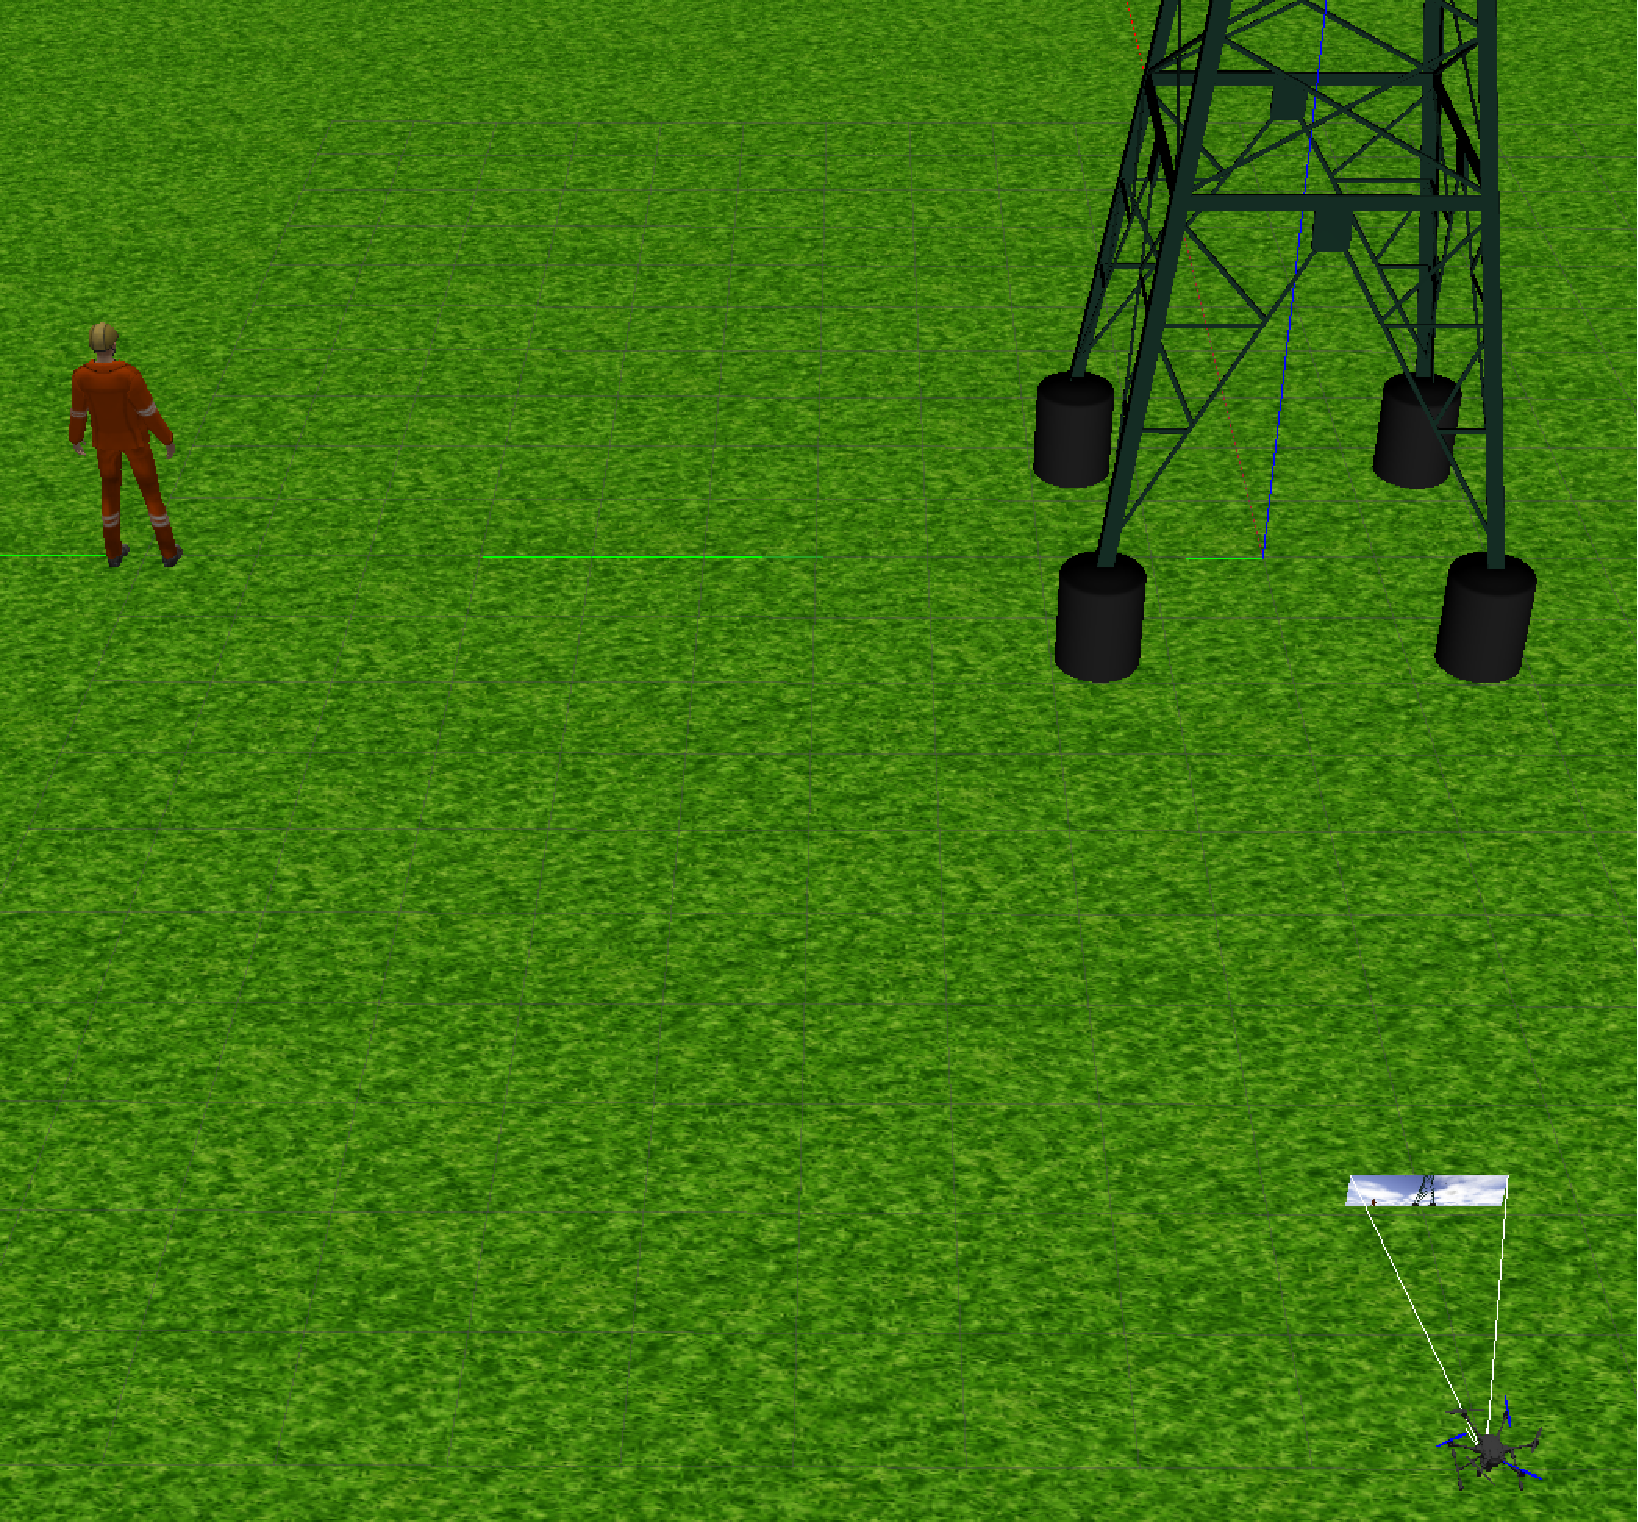
\includegraphics[width=.45\linewidth]{Results/figures/GazeboBatSta.pdf}}
    \hfill
    \subfloat[\gls{BT}'s starting status displayed with Groot]{
        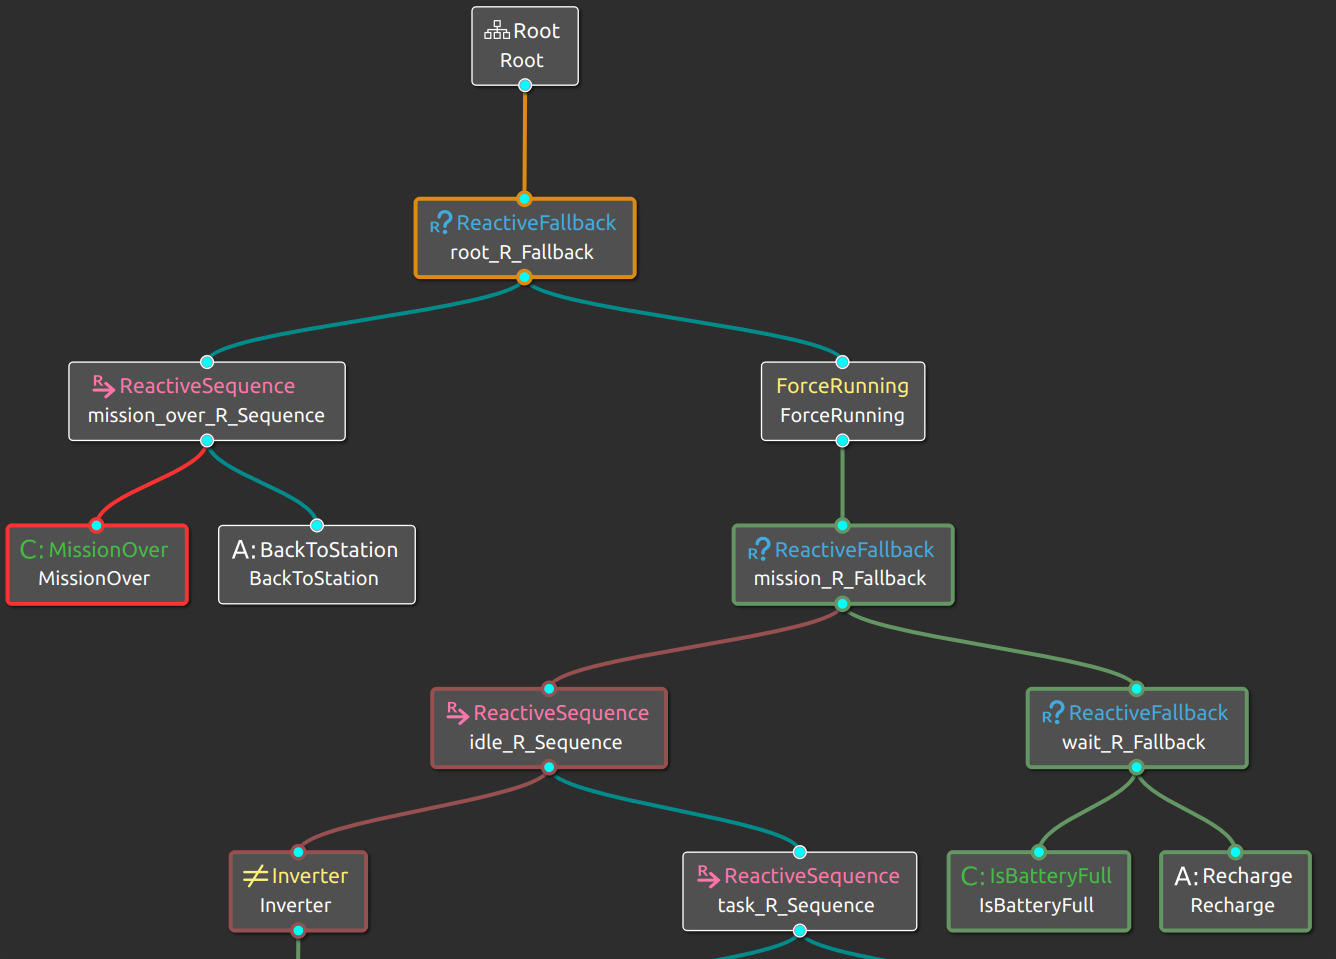
\includegraphics[width=.45\linewidth]{Results/figures/BTini.jpeg}}
    \caption{Initial status of the simulation: battery charged and no task queued.}
    \label{fig:BTinitialization}
\end{figure}

At the beginning, the \gls{UAV} has the battery charged, is landed on the charging station and has no task queued, then the \gls{BT} is returning \emph{SUCCESS} except for the \emph{Force Running} node, which keeps the \gls{BT} running by always returning \emph{RUNNING} (see Fig. \ref{fig:BTinitialization}). Note that Groot uses its own colour code to represent the result of each node in the previous tick. \emph{Green} stands for \emph{SUCCESS}, \emph{Red} for \emph{FAILURE}, \emph{Orange} for \emph{RUNNING} and \emph{White} for \emph{IDLE}. In addition, when a node is still called by a \emph{Reactive Control} node after it has finished, if the result is the same, the colour of the node is maintained but in a less intense tone. 

\begin{figure}[htbp]
    \centering
    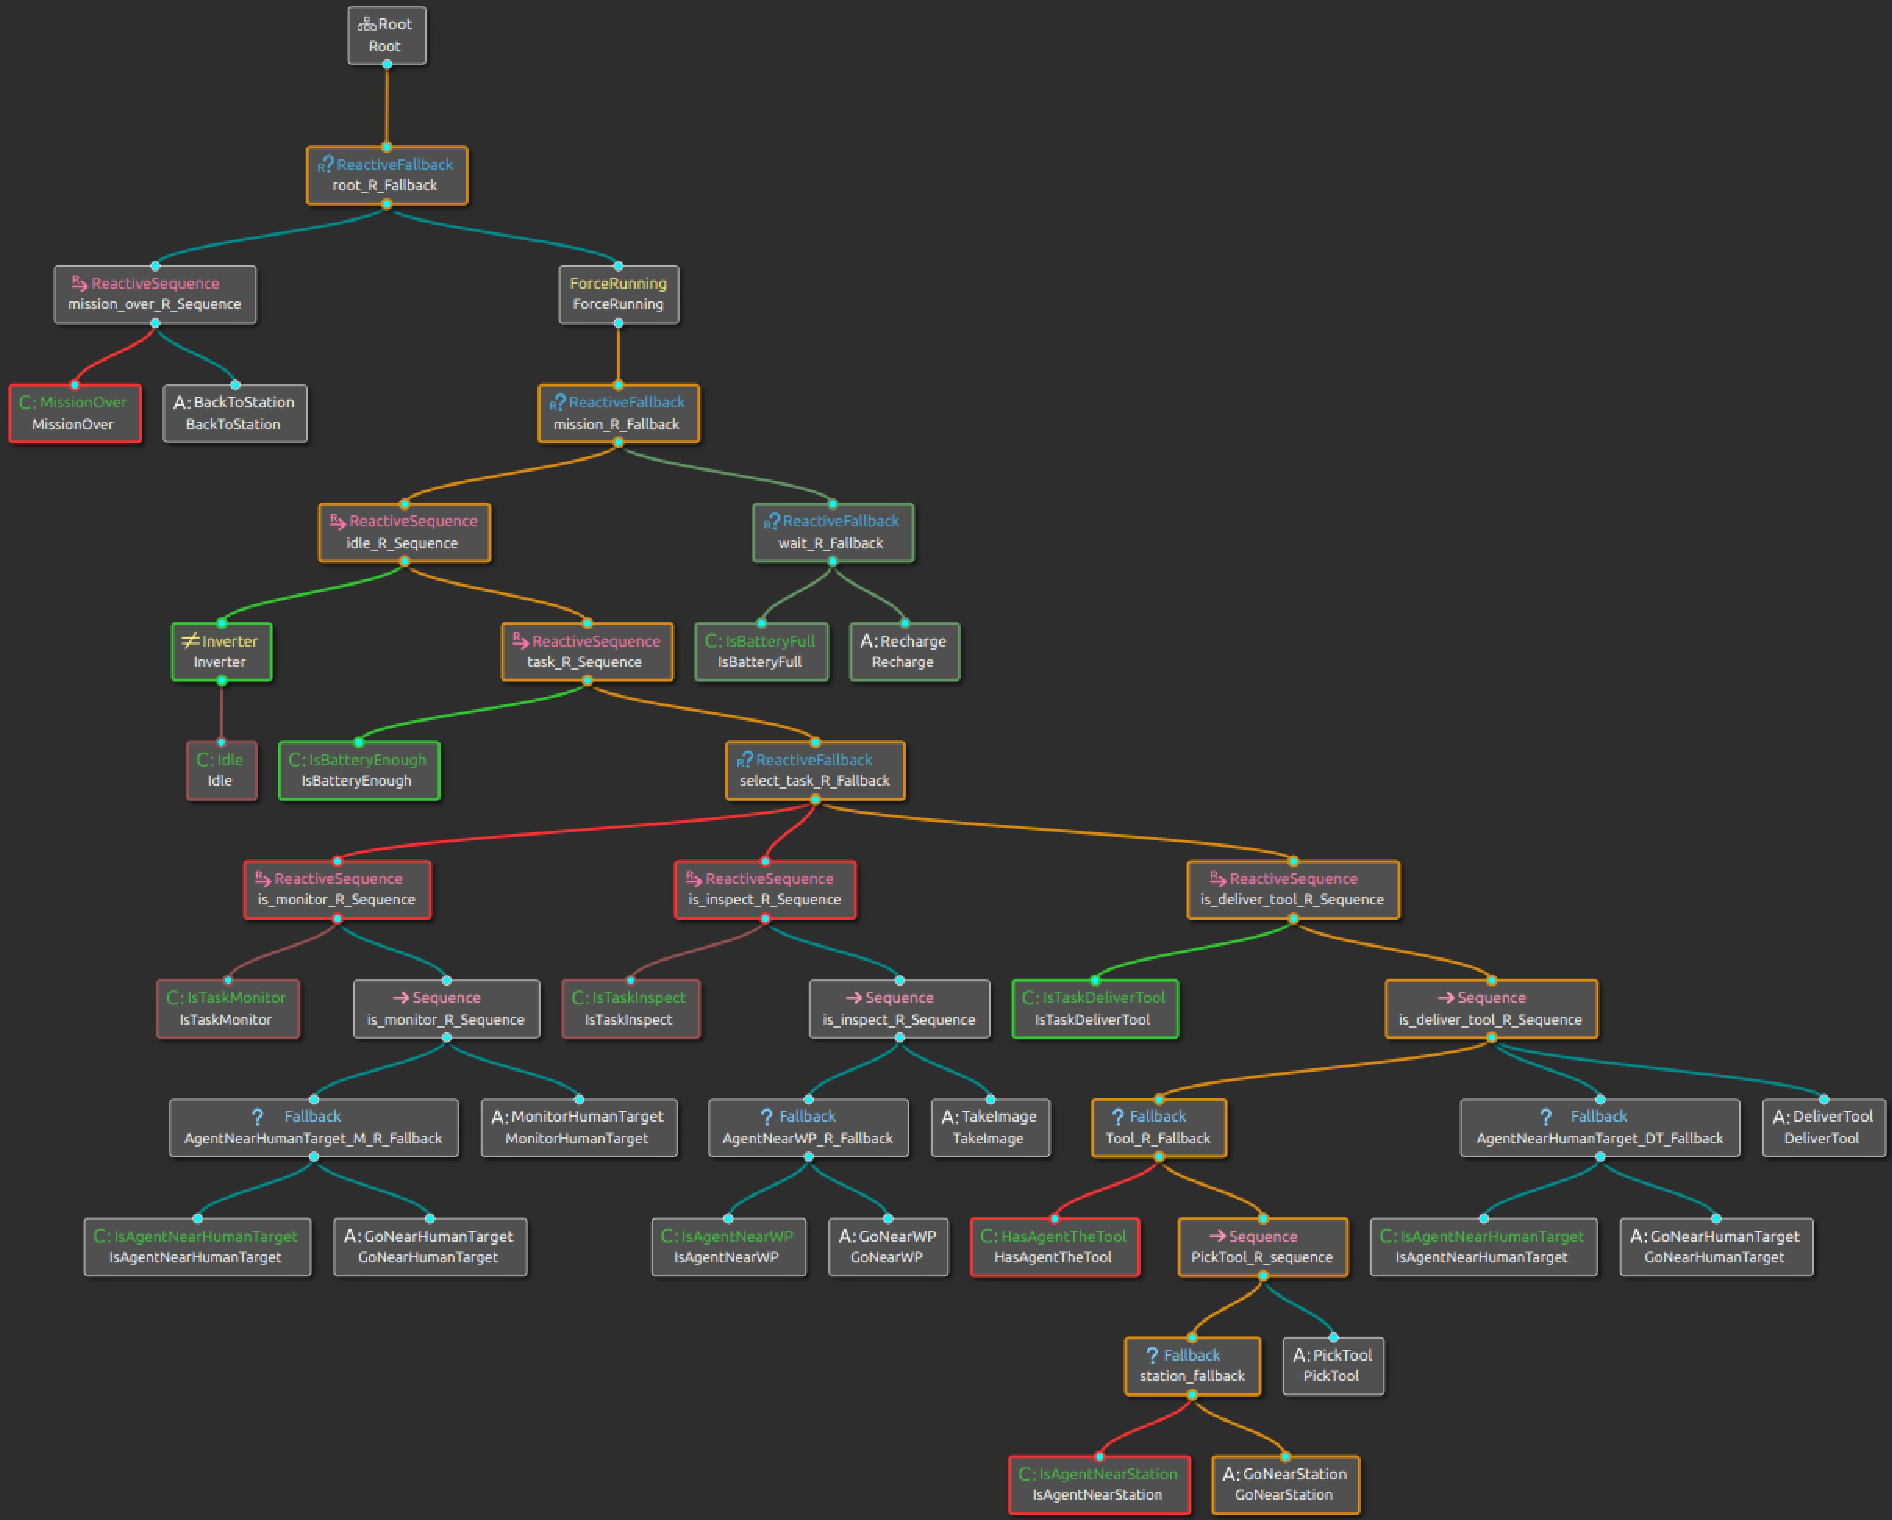
\includegraphics[width=.75\linewidth]{Results/figures/BTnoIdle.pdf}
    \caption{\gls{BT} transition from idle to \emph{Tool Delivery Task Tree}}
    \label{fig:NoIdle_DeliverToolTaskTree}
\end{figure}

For this simulation, tasks were requested from the \emph{High-Level Planner} before communication with the \emph{Agent Behaviour Manager} was established. Once the distributed block had finished initialising, communication between the two blocks could be established and with it the first task planning. While this happened, the \gls{BT} controlling the \gls{ACW} started executing and, not yet having any tasks assigned to it, directed the \gls{UAV} towards the charging station while it waited. Once the first task queue was communicated, the \gls{BT} checked which task was the first one and proceeded to execute it (see Fig. \ref{fig:NoIdle_DeliverToolTaskTree}). The code \ref{exit:newtaskqueue} shows the feedback posted by both blocks until the completion of the execution of the first task.

\begin{lstlisting}[caption={Feedback of the task planning process and communications between \emph{High-Level Planner} and \emph{Agent Behaviour Manager}at the beginning of the simulation}, breaklines=true, label=exit:newtaskqueue]
    [ INFO][/task_planner]: [Planner] Initialization complete

    [ INFO][/task_planner]: [incomingTask] Received a New Tasks:
        task_1: Deliver
            Tool: hammer (1.5kg): -2, 5, 0.9
            Human Target: human_target_1: 0, 10, 1.85
        task_2: Inspect
            Positions: (0, 0, 2) (10, 10, 2) (0, 10, 2) (10, 0, 2)
            Agent List:
        task_3: Monitor (1.5, 4)
            Human Target: human_target_1: 0, 10, 1.85
            Agent List:
    
    [ INFO][/task_planner]: [incomingTask] Allocating tasks...
    [ WARN][/task_planner]: [performTaskAllocation] No Agents connected yet. 3 pending tasks
    
    
    
    [ INFO][/uav_1/agent]: [AgentNode] uav_1 initialized. State: 0
    [ INFO][/uav_1/agent]: [Recharge] Calling take_off
    [ INFO][/uav_1/agent]: [Recharge] Moving to recharging station
    [ INFO][/uav_1/agent]: [Recharge] Calling land
    [ INFO][/uav_1/agent]: [Recharge] Charging...
    
    [ INFO][/task_planner]: [beaconCallback] New Agent connected: uav_1
    [ INFO][/task_planner]: [performTaskAllocation] Tasks Allocated:
    [ INFO][/task_planner]: [performTaskAllocation] Agent id: uav_1
        Agent type: PhysicalACW
        Task list: (3 tasks)
            task_1: DeliverTool
            task_2: Inspect
            task_3: Monitor
    
    [ INFO][/uav_1/agent]: [newTaskList] Received a NewTaskList Action
    [ INFO][/uav_1/agent]: task_1: DeliverTool
    [ INFO][/uav_1/agent]: [Recharge] halt requested
    [ INFO][/uav_1/agent]: [GoNearStation] Moving near Tool...
\end{lstlisting}

The \emph{Tool Delivery Task Tree} functioned perfectly well. In Gazebo, the movement of the \gls{ACW} from one side to the other was observed as the \gls{BT} traversed the nodes of the subtree of this task (see Fig. \ref{fig:Gazebo_DeliverTree}). In addition, the task result was checked for correct communication with the centralised block, which used the moment to re-evaluate the plan to see if it is still within the optimal plan (see code \ref{exit:tasksFInishAndReplanning}). As the plan did not change, the \gls{BT} continued to execute the queued tasks. As it has already been shown that the activation of \emph{Action} nodes in the \gls{BT} correctly moves the \gls{ACW} in the Gazebo simulation, no screenshots of the simulation are shown from now on as they are not relevant. Figure \ref{fig:Gazebo_InspectTree} shows the evolution of the \gls{BT} during the execution of the \emph{Inspection} task, for which the \gls{BT} also proved to work perfectly. 

\begin{figure}[htbp]
    \centering
    \subfloat[Initial position: charge station]{
        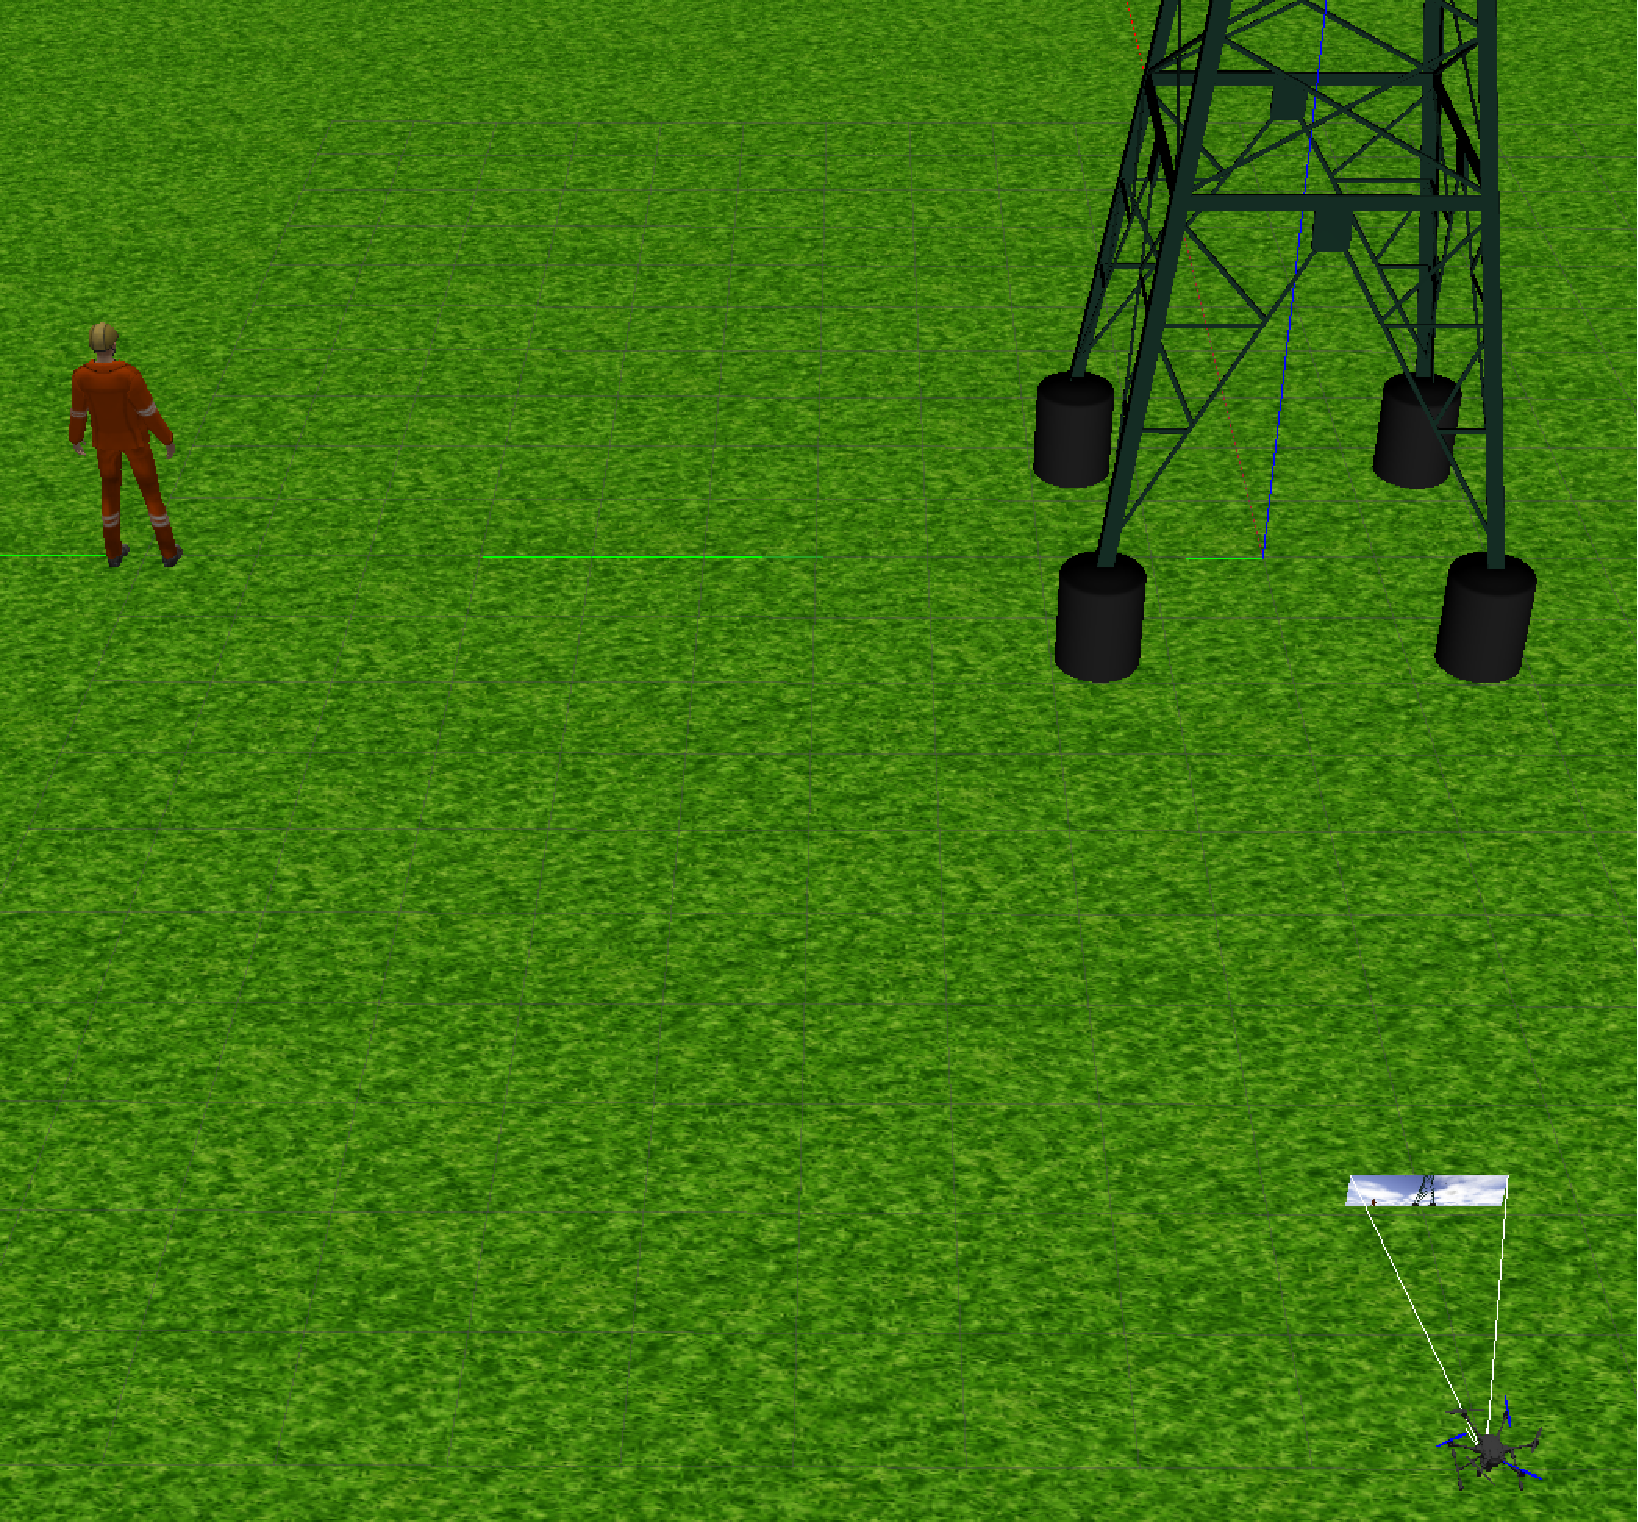
\includegraphics[width=.3\linewidth]{Results/figures/GazeboBatSta.pdf}}
    \hfill
    \subfloat[Base station: tool picking]{
        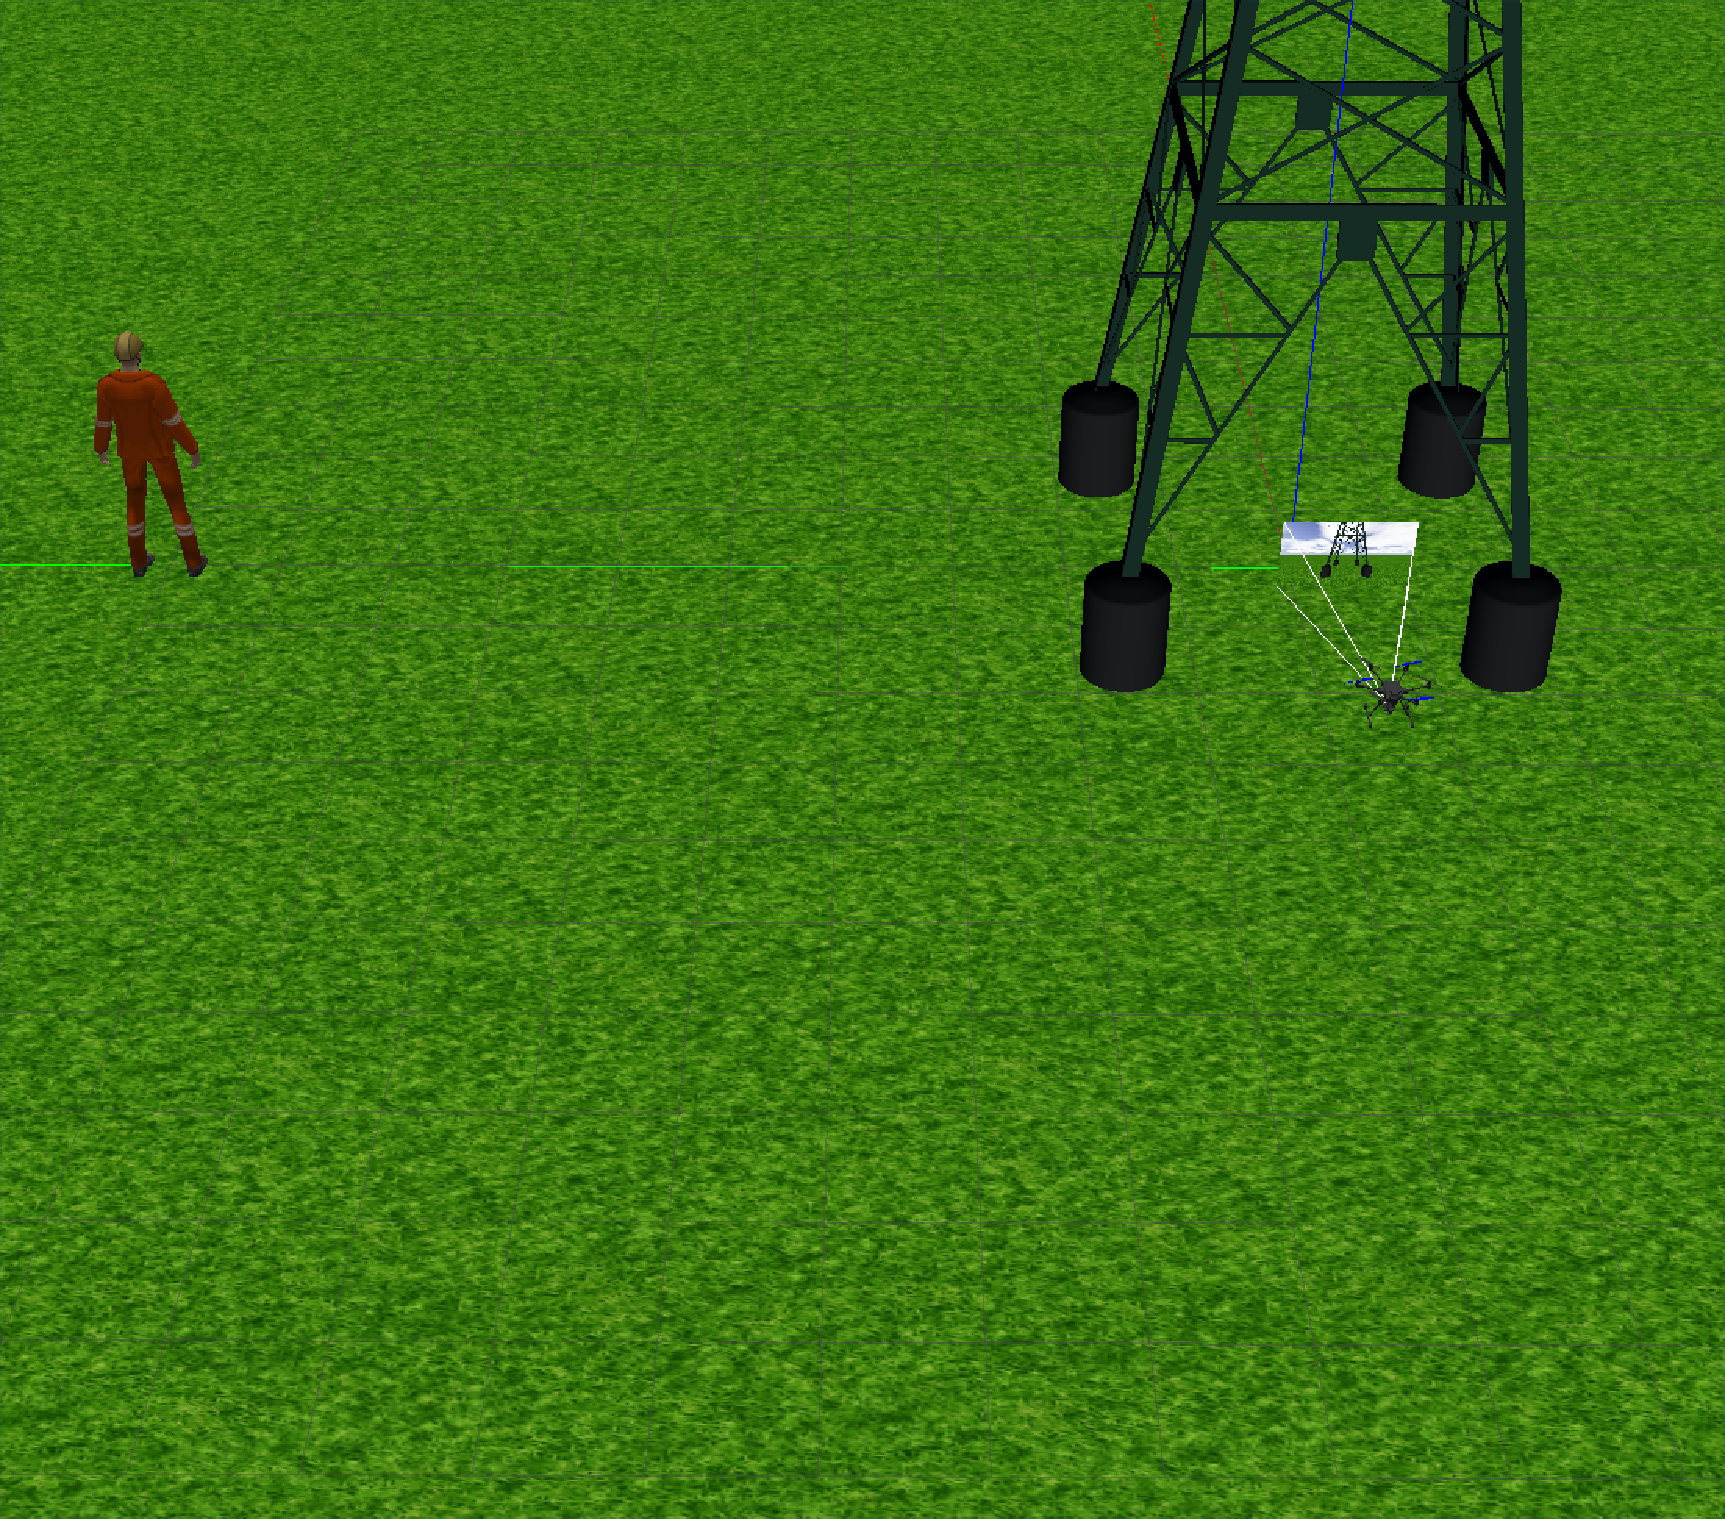
\includegraphics[width=.3\linewidth]{Results/figures/GazeboTool.pdf}}
    \hfill
    \subfloat[Human target position: tool delivery]{
        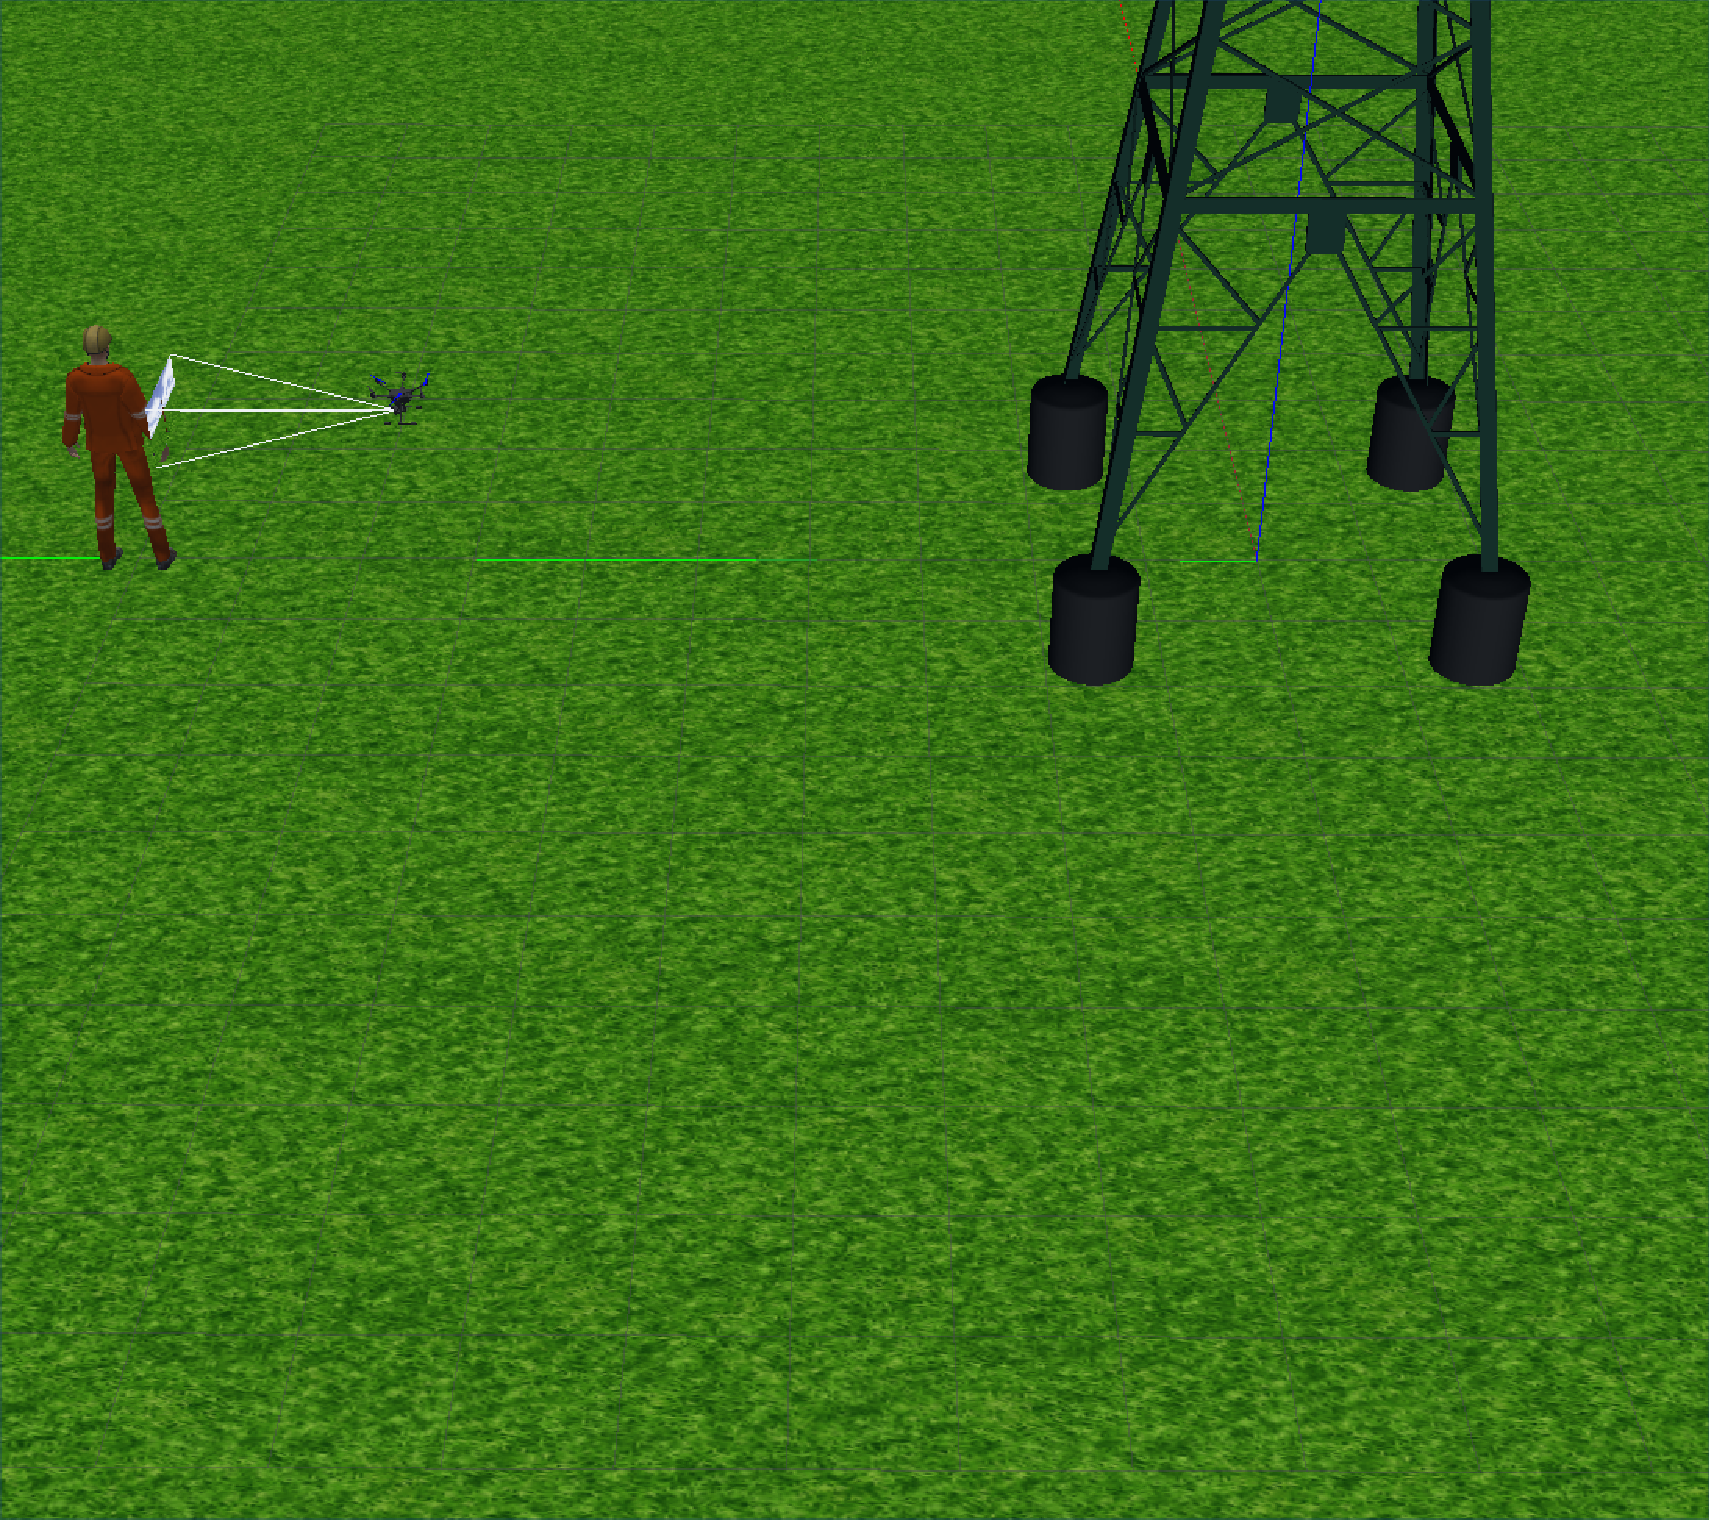
\includegraphics[width=.3\linewidth]{Results/figures/GazeboHuman.pdf}}
    \hfill
    \\
    \subfloat[Activation of \emph{Go Near Station} action after checking \emph{Has ACW the tool} and \emph{Is ACW near Station} conditions]{
        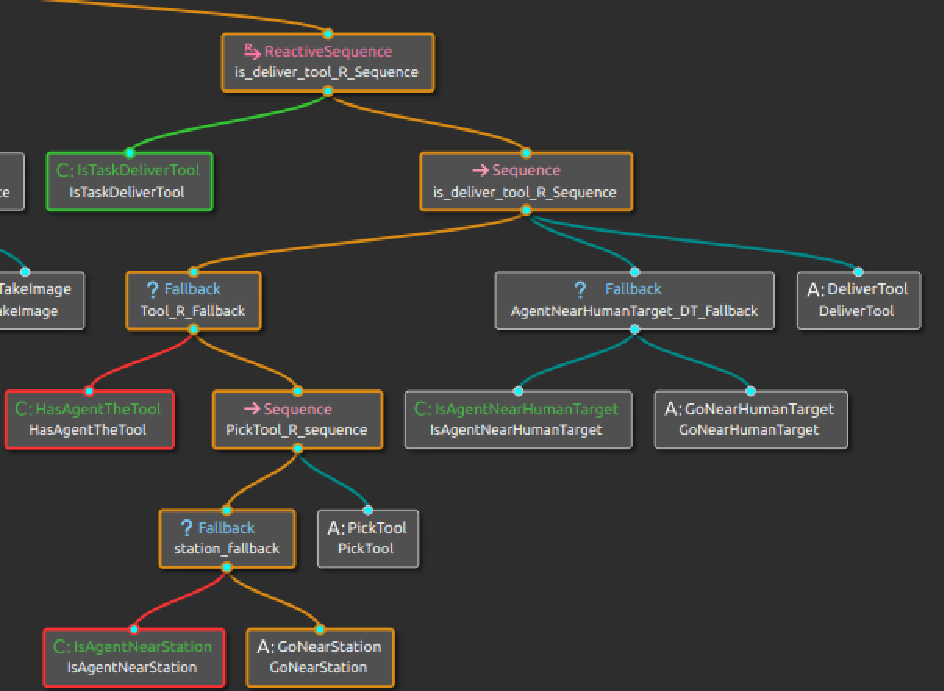
\includegraphics[width=.45\linewidth]{Results/figures/BTDTGNS.pdf}}
    \hfill
    \subfloat[Activation of \emph{Pick Tool} action after arriving at the base station]{
        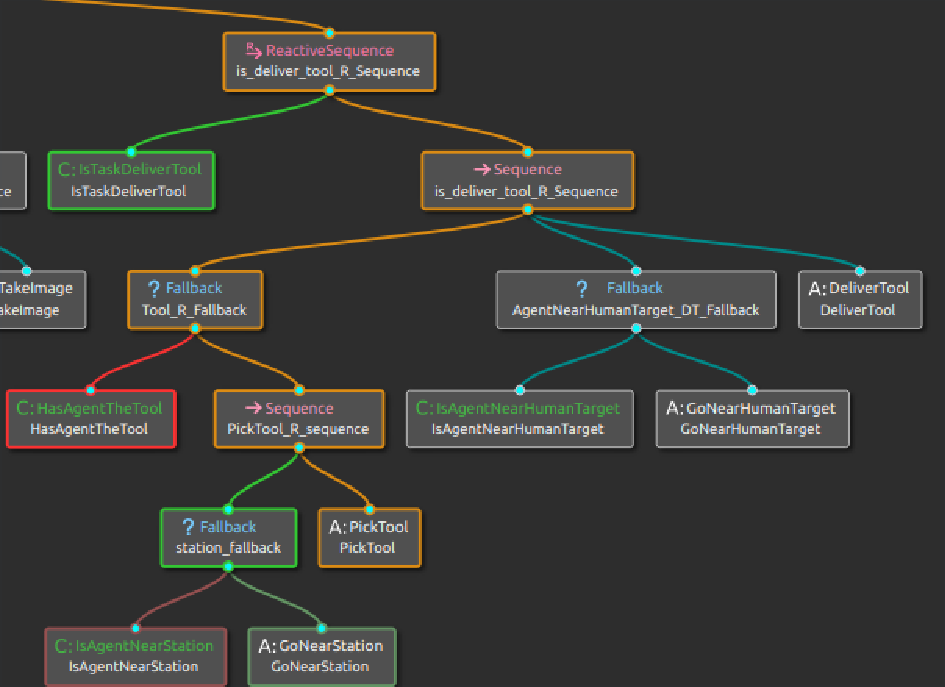
\includegraphics[width=.45\linewidth]{Results/figures/BTDTPT.pdf}}
    \\
    \subfloat[Activation of \emph{Go Near Human Target} action after having the tool and checking \emph{Is ACW Human Target} condition]{ 
        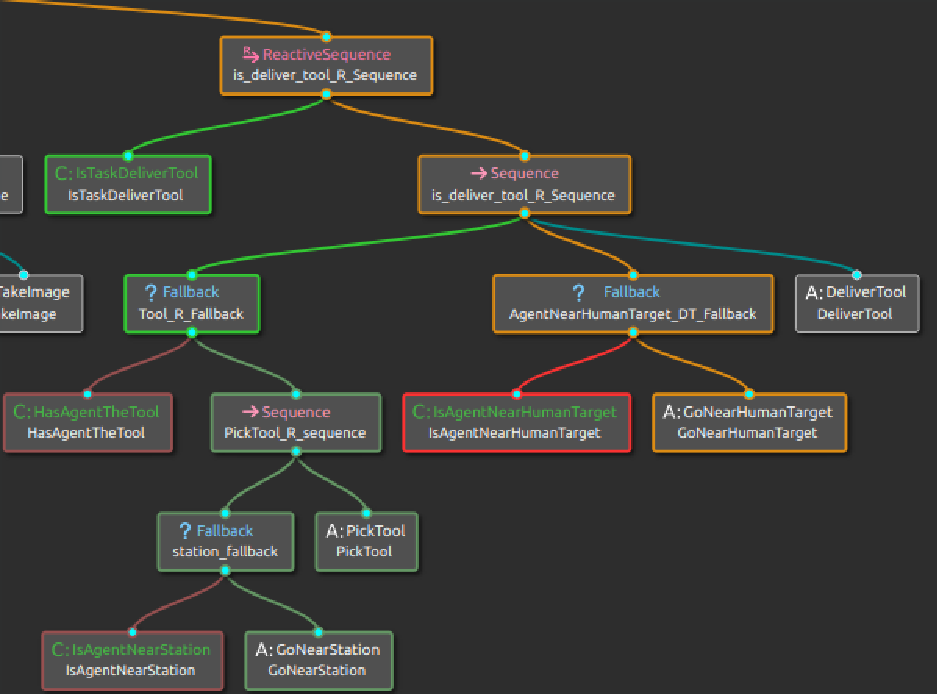
\includegraphics[width=.45\linewidth]{Results/figures/BTDTGNHT.pdf}}
    \hfill
    \subfloat[Activation of \emph{Deliver Tool} action after arriving near human target having the tool]{
        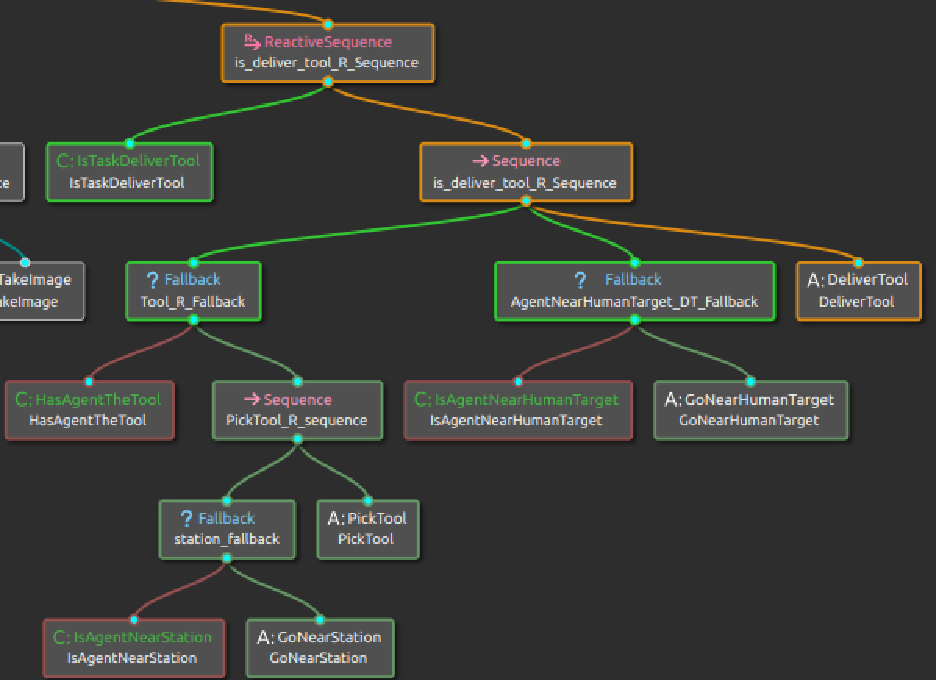
\includegraphics[width=.45\linewidth]{Results/figures/BTDTDT.pdf}}
    \caption{Evolution of the simulation during the execution of the \emph{Tool Delivery Task Tree}}
    \label{fig:Gazebo_DeliverTree}
\end{figure}

\begin{figure}[htbp]
    \centering
    \subfloat[Activation of \emph{Go Near WP} action after checking \emph{Is Agent Near WP} condition]{
        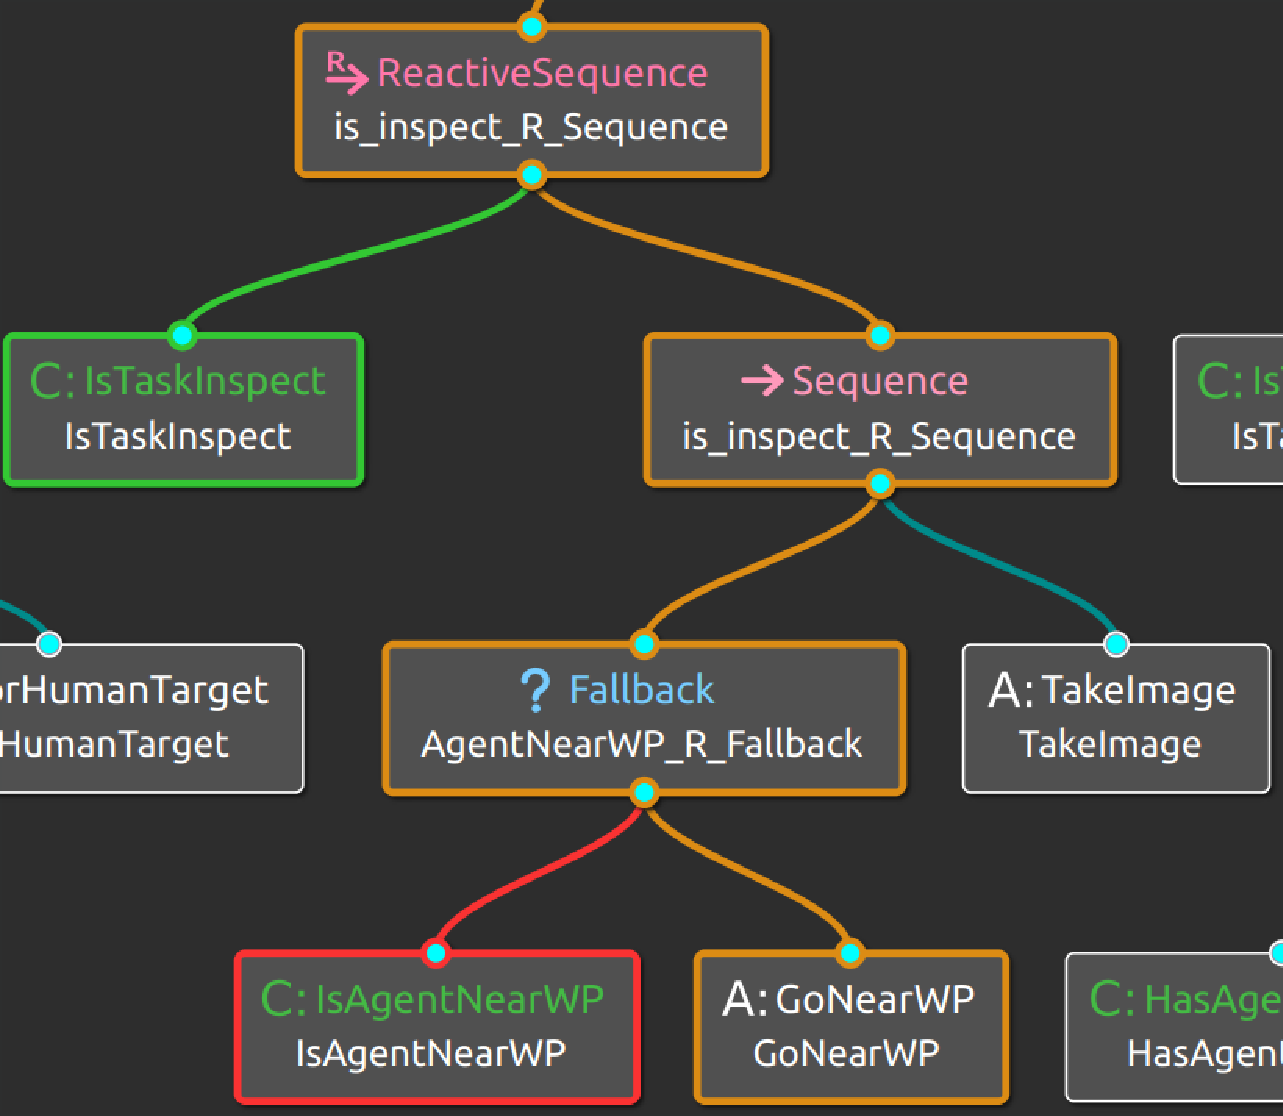
\includegraphics[width=.45\linewidth]{Results/figures/BTIGNWP.pdf}}
    \hfill
    \subfloat[Activation of \emph{Take Image} action after arriving near WP]{
        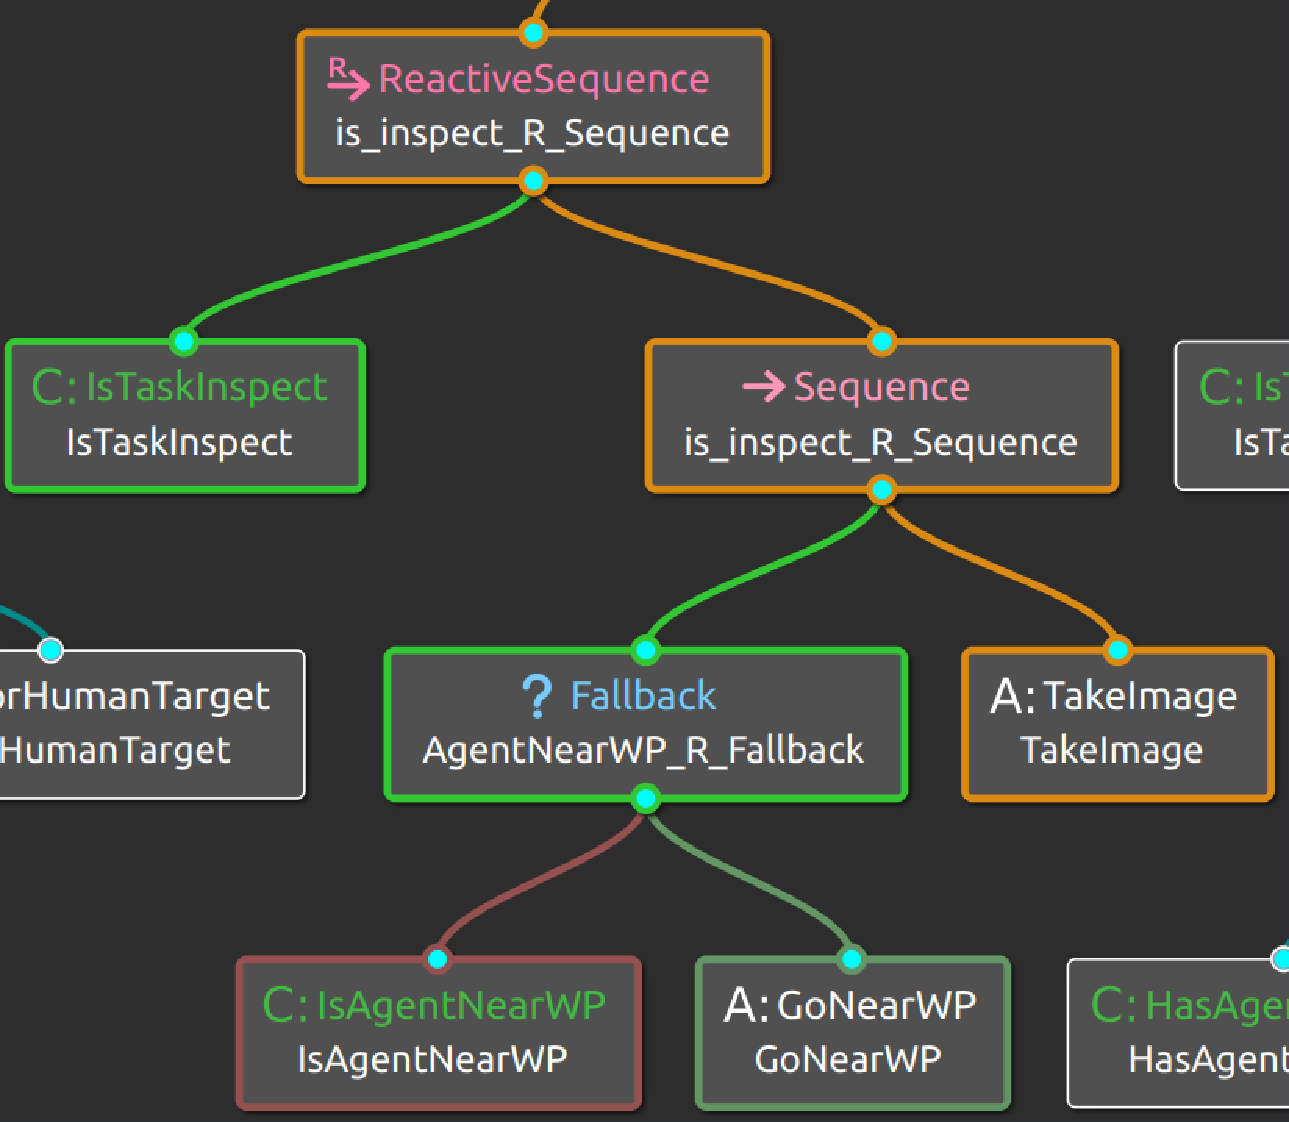
\includegraphics[width=.45\linewidth]{Results/figures/BTITI.pdf}}
    \caption{Evolution of the \gls{BT} during the execution of the \emph{Inspection Task Tree}}
    \label{fig:Gazebo_InspectTree}
\end{figure}

\begin{lstlisting}[caption={Feedback messages printed out during replanning that were carried out when tasks were completed}, breaklines=true, label=exit:tasksFInishAndReplanning]
    [ INFO][/task_planner]: [taskResultCB] (uav_1) task_1(DeliverTool) SUCCEEDED. Reallocating just in case...
    [ INFO][/task_planner]: [performTaskAllocation] Tasks Allocated:
    [ INFO][/task_planner]: [performTaskAllocation] Agent id: uav_1
        Agent type: PhysicalACW
        Task list: (2 tasks)
            task_2: Inspect
            task_3: Monitor
    
    [ INFO][/task_planner]: [taskResultCB] (uav_1) task_2(Inspect) SUCCEEDED. Reallocating just in case...
    [ INFO][/task_planner]: [performTaskAllocation] Tasks Allocated:
    [ INFO][/task_planner]: [performTaskAllocation] Agent id: uav_1
        Agent type: PhysicalACW
        Task list: (1 tasks)
            task_3: Monitor
\end{lstlisting}

Finally, when this task was finished, the \gls{BT} proceeded to execute the \emph{Safety Monitoring} task, which was also carried out without problems (see Fig. \ref{fig:Gazebo_MonitorTree}). Code \ref{exit:firstPlanFeedback} shows all feedback messages printed by the \emph{Agent Behaviour Manager} during the execution of the whole plan. 

\begin{figure}[htbp]
    \centering
    \subfloat[Activation of \emph{Go Near Human Target} action after checking \emph{Is Agent Near Human Target} condition]{
        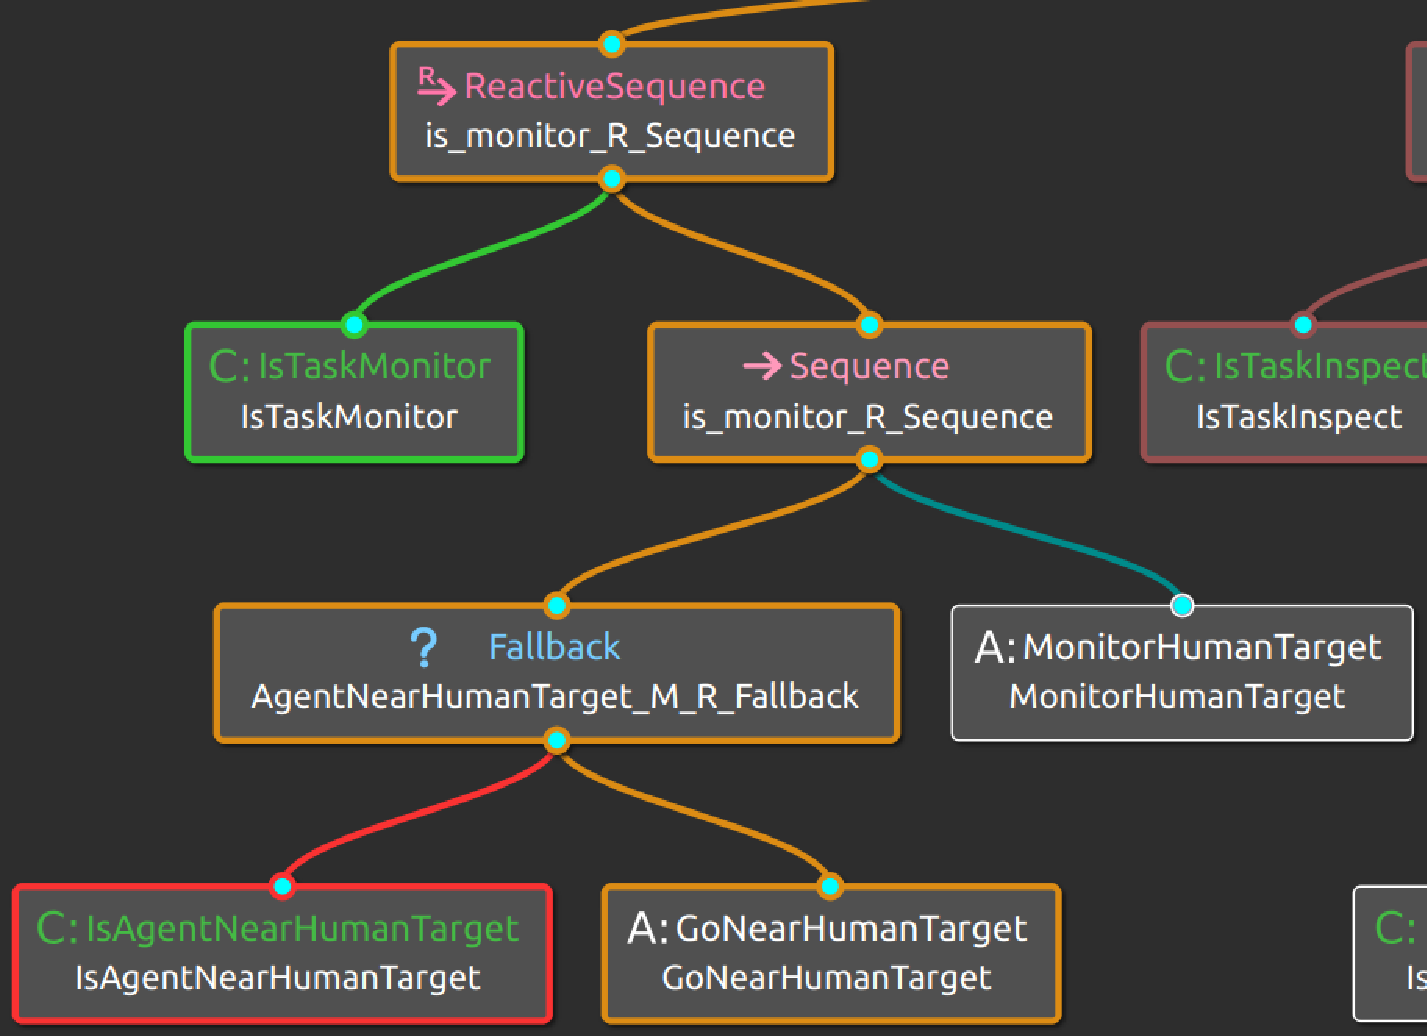
\includegraphics[width=.45\linewidth]{Results/figures/BTMGNHT.pdf}}
    \hfill
    \subfloat[Activation of \emph{Monitor Human Target} action after arriving near Human Target]{
        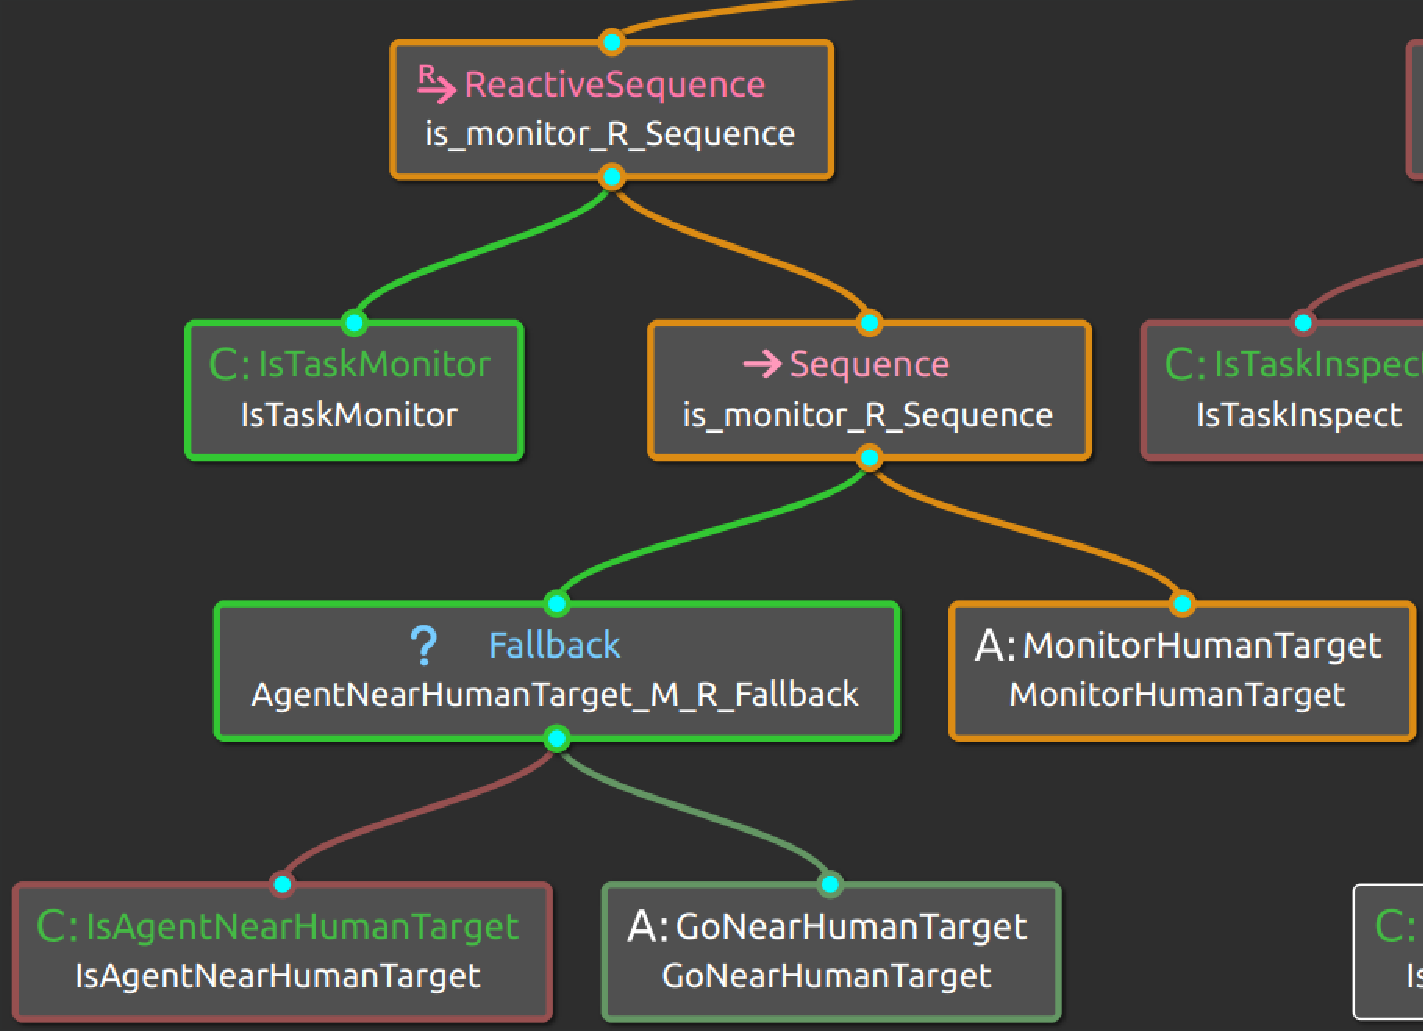
\includegraphics[width=.45\linewidth]{Results/figures/BTMMHT.pdf}}
    \caption{Evolution of the \gls{BT} during the execution of the \emph{Monitoring Task Tree}}
    \label{fig:Gazebo_MonitorTree}
\end{figure}

\begin{lstlisting}[caption={Feedback messages printed by the \emph{Agent Behaviour Manager} during the execution of the whole plan}, breaklines=true, label=exit:firstPlanFeedback]
    [ INFO][/uav_1/agent]: [newTaskList] Received a NewTaskList Action
    [ INFO][/uav_1/agent]: task_1: DeliverTool
    [ INFO][/uav_1/agent]: [Recharge] halt requested
    [ INFO][/uav_1/agent]: [GoNearStation] Moving near Tool...
    [ INFO][/uav_1/agent]: [PickTool] Calling Lower-level controllers...
    [ INFO][/uav_1/agent]: [PickTool] PICK TOOL FINISHED
    [ INFO][/uav_1/agent]: [GoNearHumanTarget] Moving near HT...
    [ INFO][/uav_1/agent]: [DeliverTool] Calling Lower-level controllers...
    [ INFO][/uav_1/agent]: [DeliverTool] DELIVER TOOL TASK FINISHED (true)
    [ INFO][/uav_1/agent]: task_2: Inspect
    [ INFO][/uav_1/agent]: [GoNearWP] Moving near WP...
    [ INFO][/uav_1/agent]: [TakeImage] Calling Lower-level controllers...
    [ INFO][/uav_1/agent]: [TakeImage] INSPECT TASK FINISHED (true)
    [ INFO][/uav_1/agent]: task_3: Monitor
    [ INFO][/uav_1/agent]: [GoNearHumanTarget] Moving near HT...
    [ INFO][/uav_1/agent]: [MonitorHumanTarget] Calling Lower-level controllers...
\end{lstlisting}

\emph{Safety Monitoring} task ends when the operator requests it, so the fake block pretending to be the low-level controller for this task is programmed so that the task never ends. This task remains in the pending tasks queue until the mission is completed or it is overwritten by a task of another type with the same \gls{ID}, which is a contemplated case for which the planner is prepared and warns the operators that an unfinished task is going to be deleted. Since during planning, tasks are assigned in order, the non-completion of this task is not a problem for the execution of other tasks, but an opportunity to study in a controlled way the emergency protocols and the response of both blocks to different unforeseen events.

It should be noted that if at some point the \gls{ACW} completed all the pending tasks and became \emph{Idle} again, it would automatically go to the charging station to recharge the battery while waiting for a new task to arrive. To test how well this works, a simulation was performed in which a single \emph{Inspection} task was requested in order to wait for the \gls{UAV} to become \emph{Idle}. The result of this test can be seen in figure \ref{fig:chargeBecouseIdle}.

\begin{figure}[htbp]
    \centering
    \subfloat[\emph{Inspection} task is running]{
        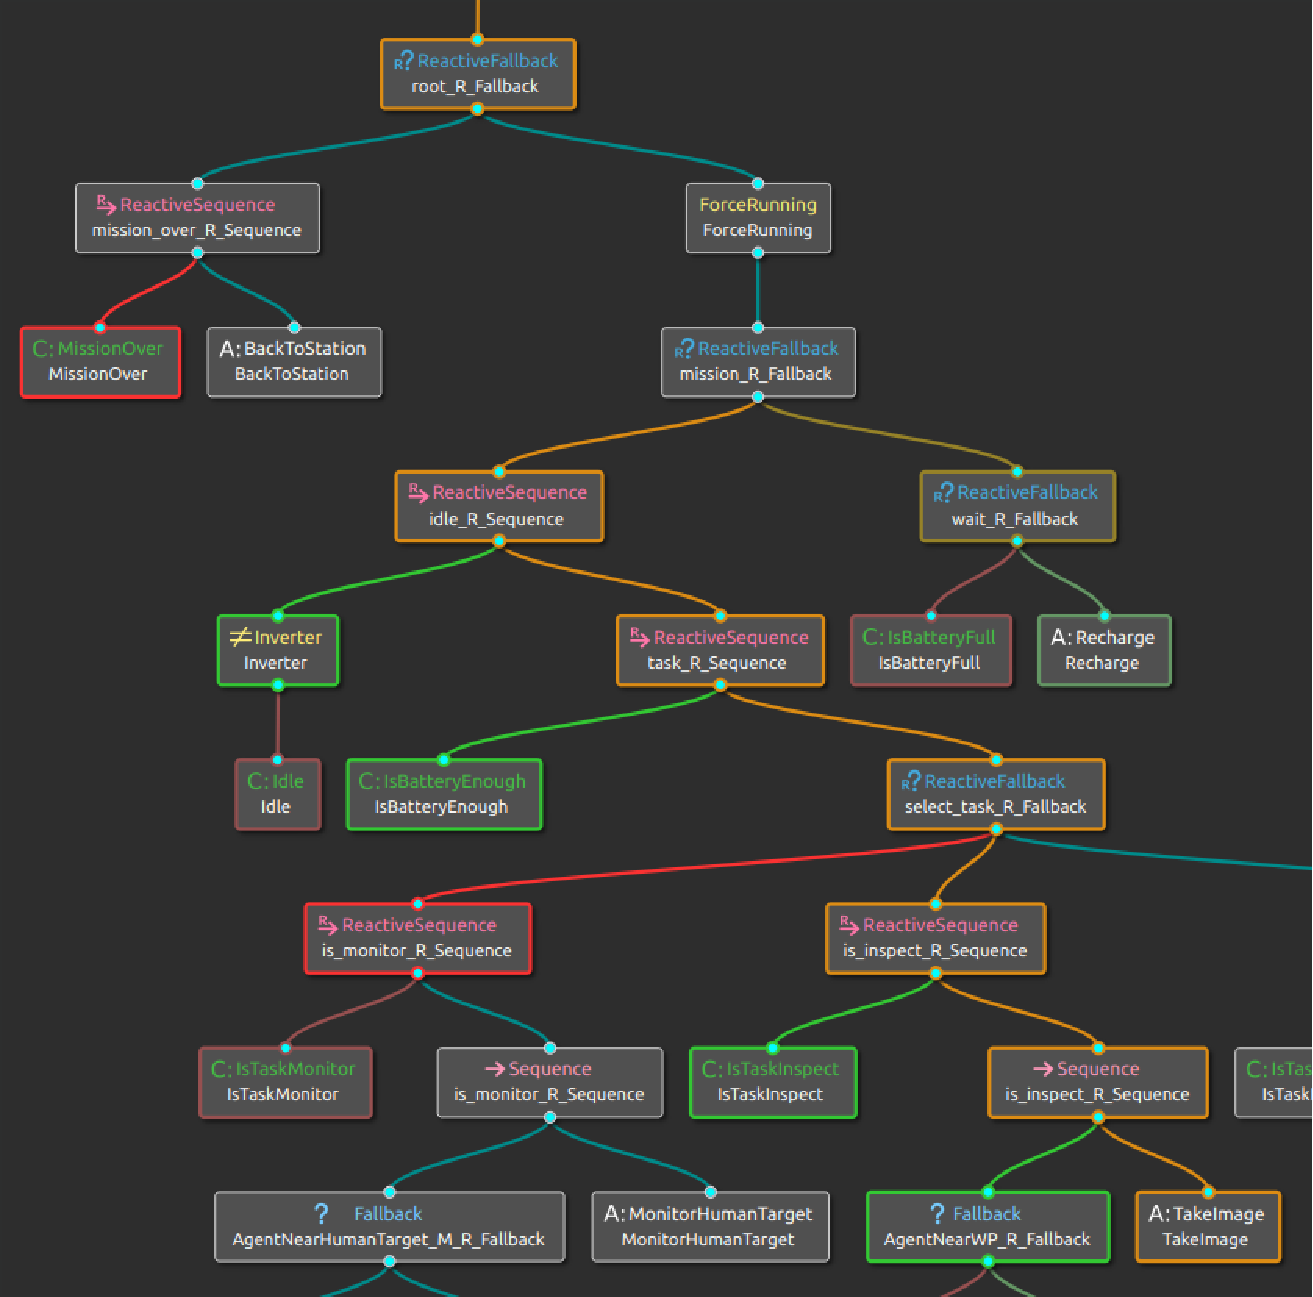
\includegraphics[width=.3\linewidth]{Results/figures/BTTaskRunnin.pdf}}
    \hfill
    \subfloat[\emph{Inspection} task finish and returs \emph{SUCCESS}]{
        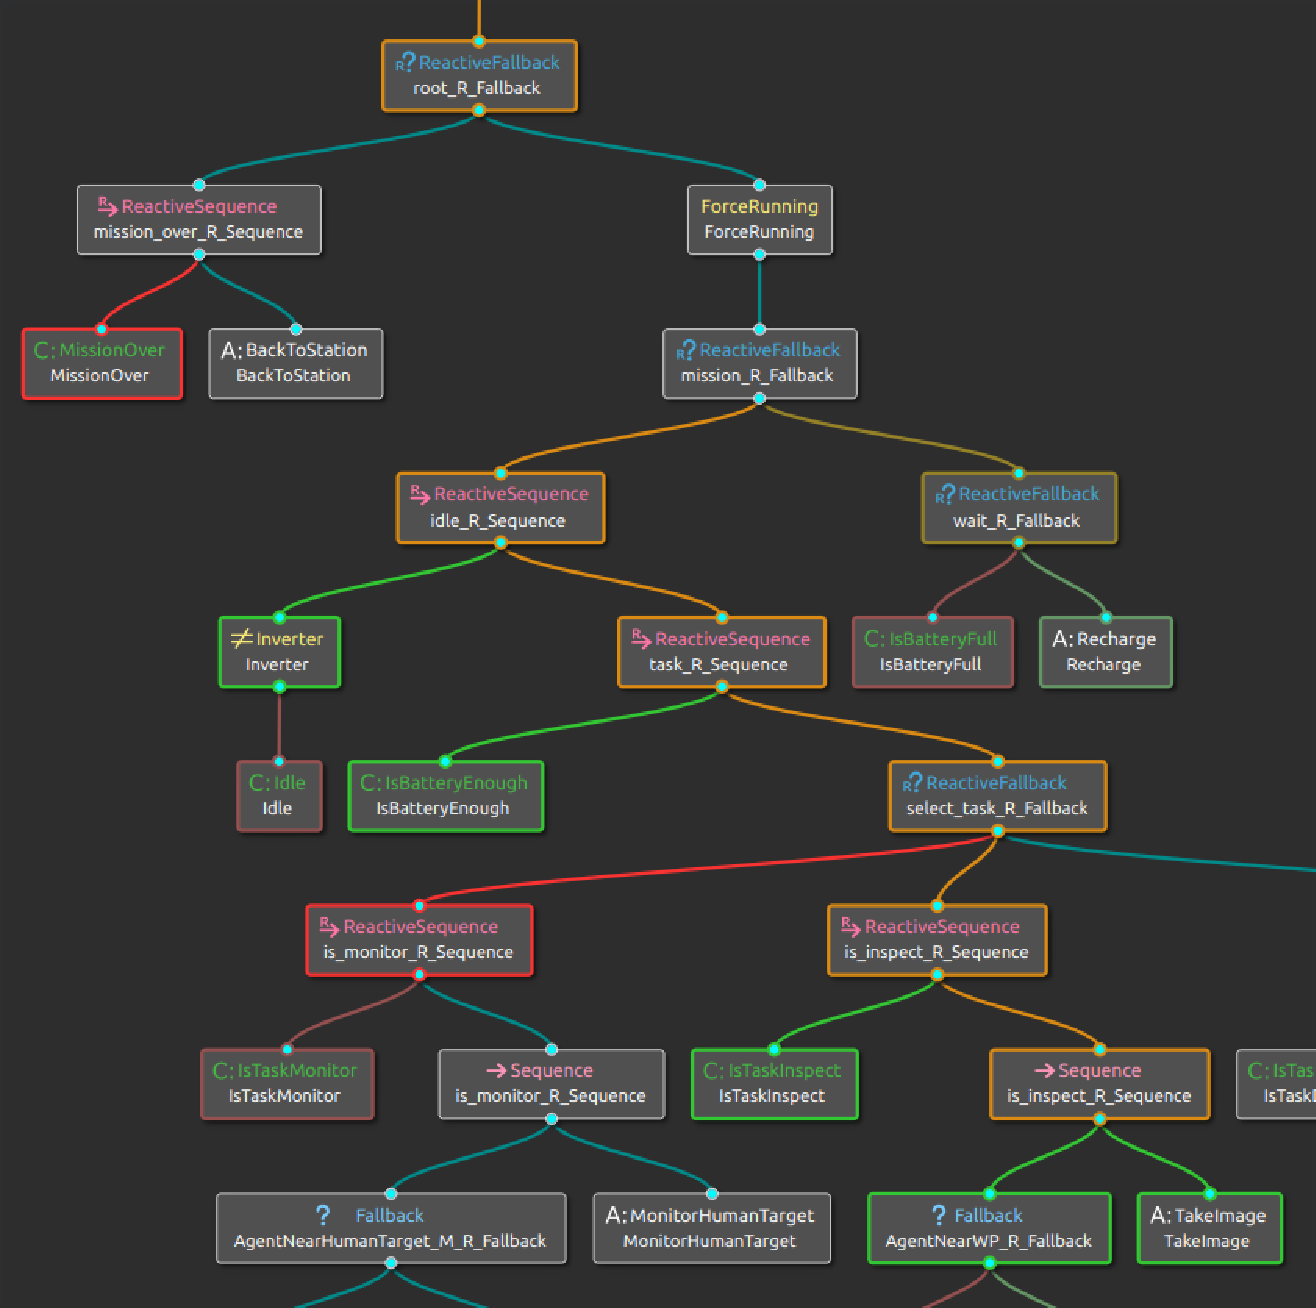
\includegraphics[width=.3\linewidth]{Results/figures/BTTaskSuccess.pdf}}
    \hfill
    \subfloat[As \gls{ACW} is now \emph{Idle}, \emph{Recharge} node is executed]{
        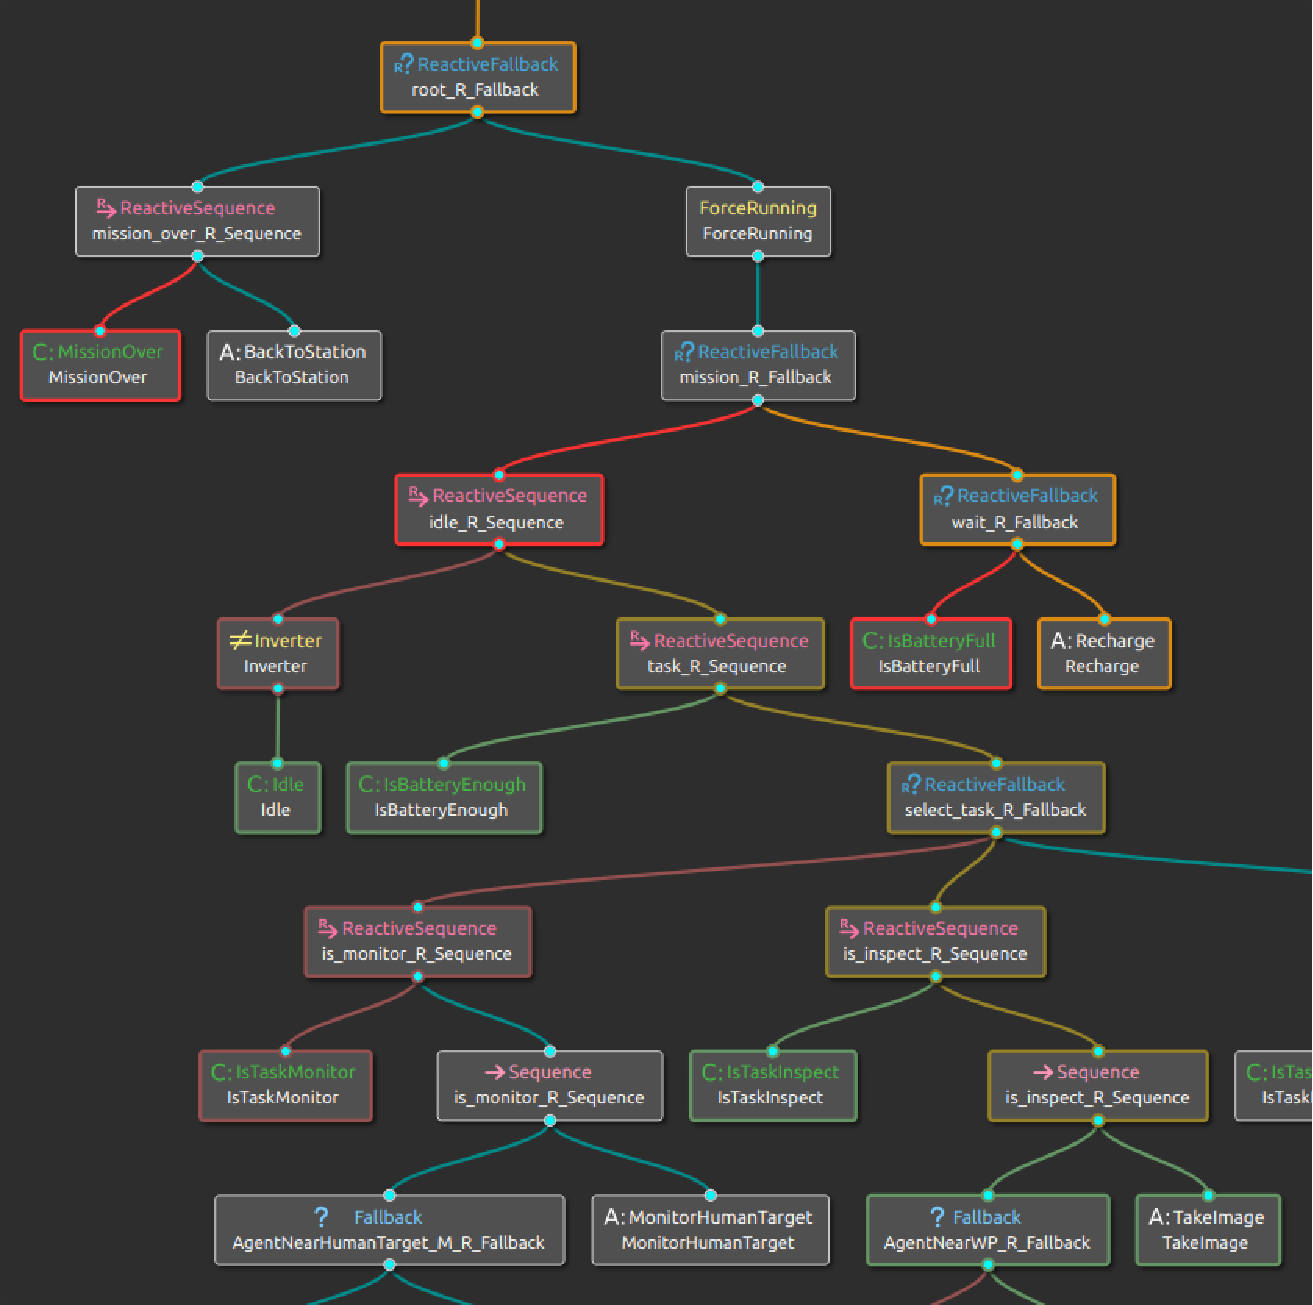
\includegraphics[width=.3\linewidth]{Results/figures/BTChargeBecIdle.pdf}}
    \caption{\gls{BT} leads the \gls{UAV} to the charging station after running out of assigned tasks}
    \label{fig:chargeBecouseIdle}
\end{figure}

Once it had been verified that the system worked well in the absence of unforeseen events, the system was tested in all kinds of situations. First, the \gls{BT}'s ability to stop the current task and switch to the execution of the new task in the event of a change of plans was tested. This was done by first requesting a \emph{Safety Monitoring} task and then requesting a \emph{Tool Delivery} task, which, having a higher priority, will move the previous task from the top of the queue. Both figure \ref{fig:event_ChangeOfPlans} and code \ref{exit:event_ChangeOfPlans} show how, after the replanning and the arrival of the new queue, the \gls{BT} stopped the task being executed by the \gls{ACW}, a \emph{Safety Monitoring} task in this case, and proceeded with the execution of the \emph{Tool Delivery} task, which now occupies the first place in the queue.

\begin{lstlisting}[caption={Feedback messages printed after a change of plans. \emph{Tool Delivery} task displaces \emph{Safety Monitoring} task}, breaklines=true, label=exit:event_ChangeOfPlans]
    [ INFO][/task_planner]: [incomingTask] Received a New Task:
        task_4: Deliver
            Tool: hammer (1.5kg): -2, 5, 0.9
            Human Target: human_target_1: 0, 10, 1.85

    [ INFO][/task_planner]: [incomingTask] Allocating tasks...
    [ INFO][/task_planner]: [performTaskAllocation] Tasks Allocated:
    [ INFO][/task_planner]: [performTaskAllocation] Agent id: uav_1
        Agent type: PhysicalACW
        Task list: (2 tasks)
            task_4: DeliverTool
            task_3: Monitor

    [ INFO][/uav_1/agent]: [newTaskList] Received a NewTaskList Action
    [ INFO][/uav_1/agent]: task_4: DeliverTool
    [ INFO][/uav_1/agent]: [MonitorHumanTarget] halt requested
    [ INFO][/uav_1/agent]: [MonitorHumanTarget] MONITOR TASK FINISHED (false)
    [ INFO][/task_planner]: [taskResultCB] (uav_1) task_3 (Monitor) in uav_1 FAILED but seems to be planned
    [ INFO][/uav_1/agent]: [GoNearStation] Moving near Tool...
    [ INFO][/uav_1/agent]: [PickTool] Calling Lower-level controllers...
\end{lstlisting}

\begin{figure}[htbp]
    \centering
    \subfloat[\emph{Safety Monitoring} tree running]{
        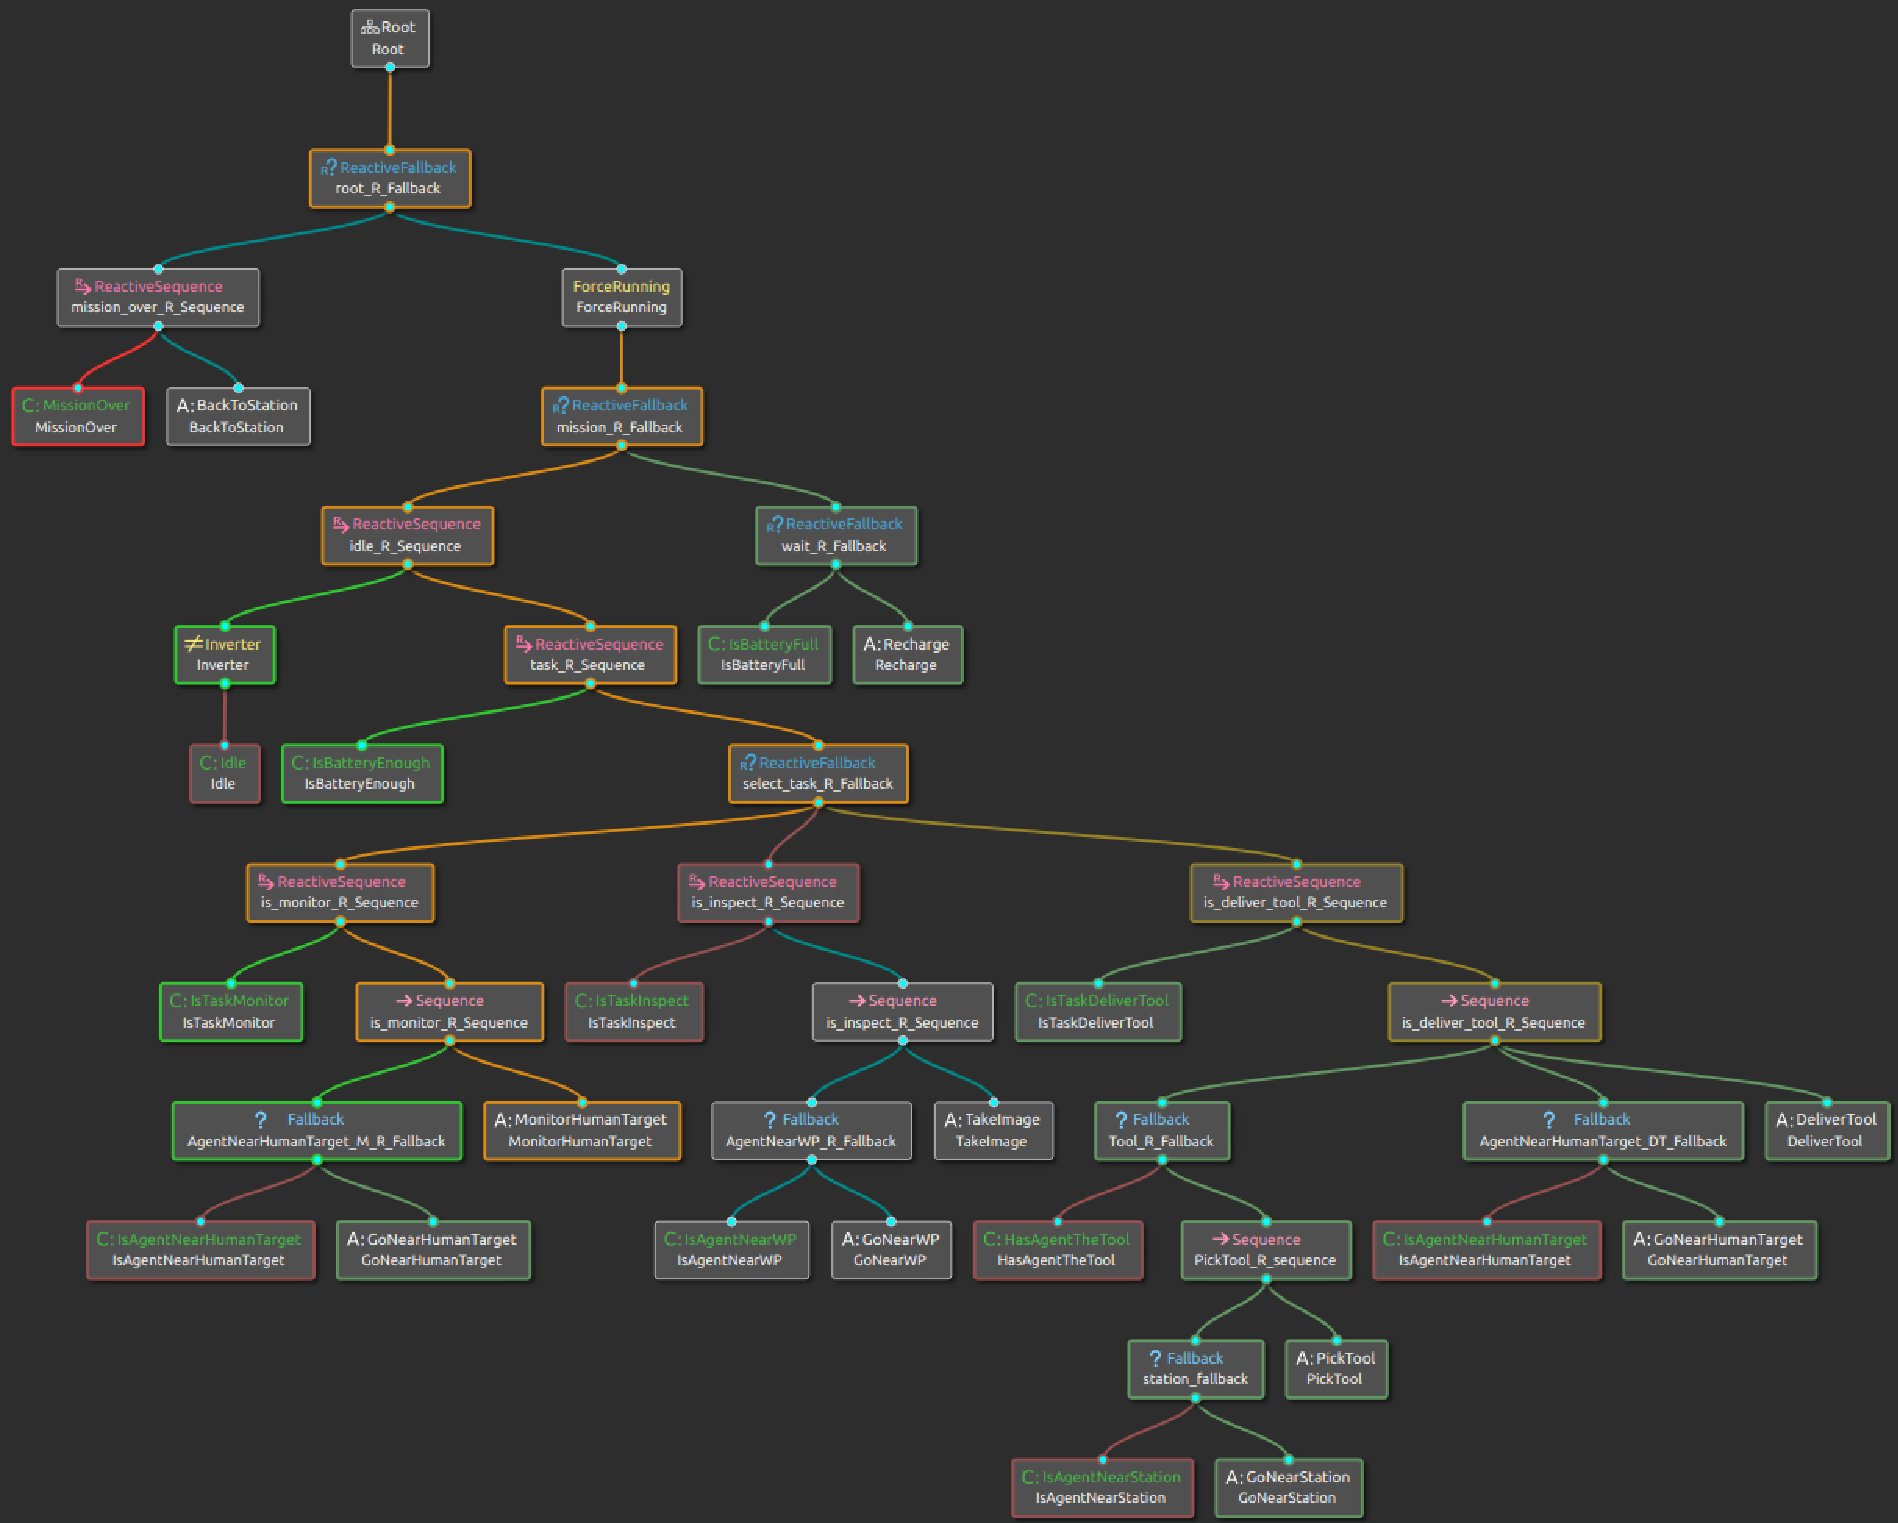
\includegraphics[width=.3\linewidth]{Results/figures/BTImprevistoMDT_1.pdf}}
    \hfill
    \subfloat[\emph{Safety Monitoring} tree is halted becouse a \emph{Tool Delivery} task took the first place in the queue]{
        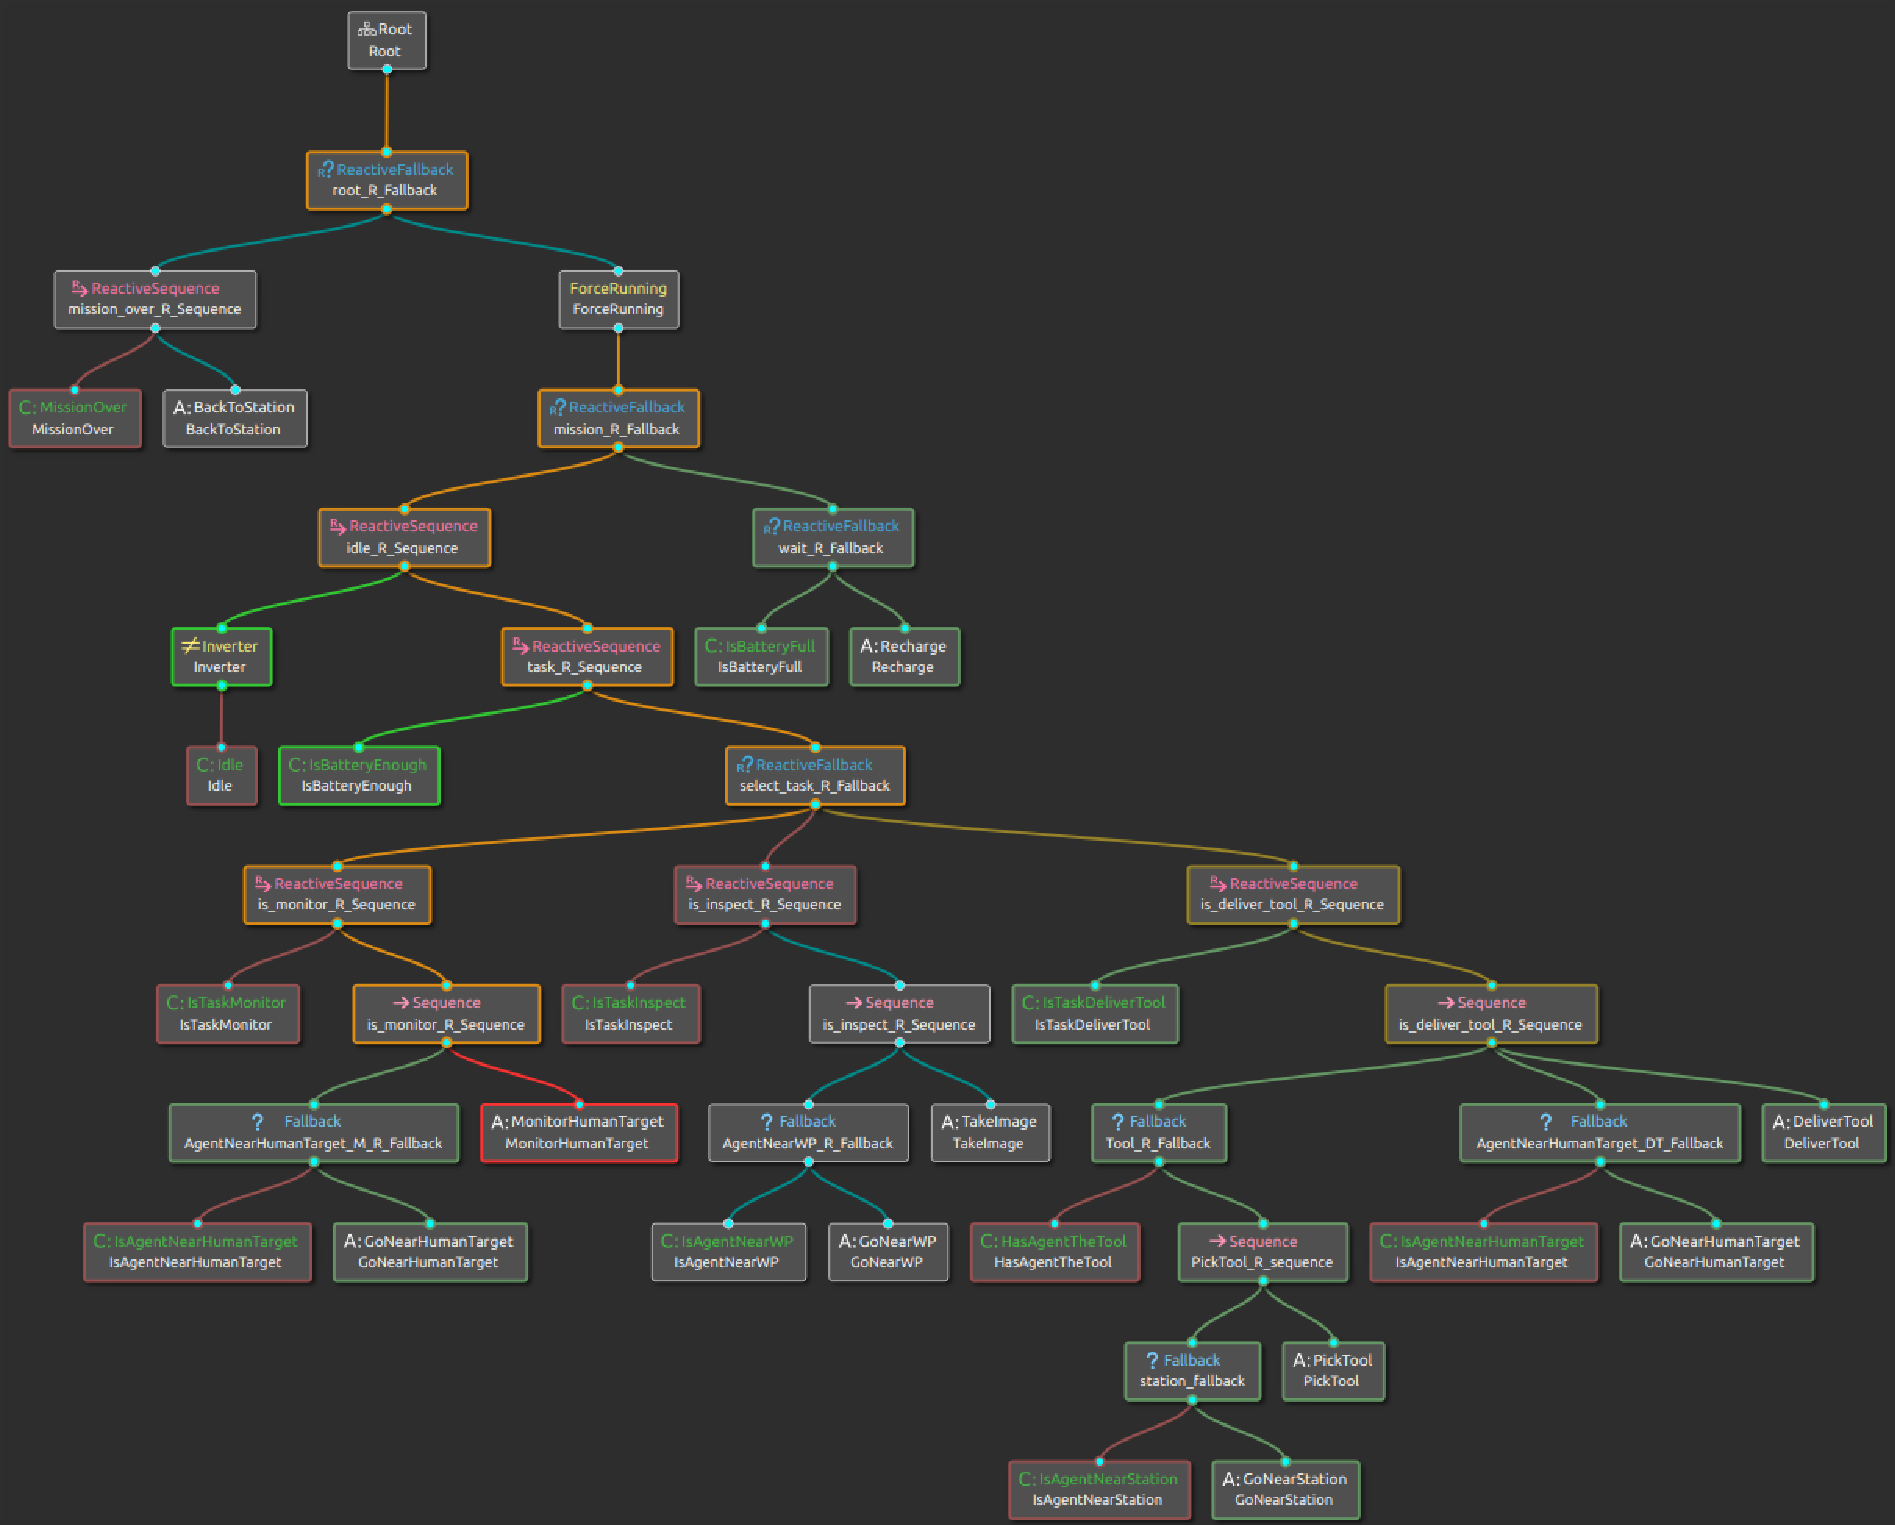
\includegraphics[width=.3\linewidth]{Results/figures/BTImprevistoMDT_2.pdf}}
    \hfill
    \subfloat[\emph{Tool Delivery} tree running]{
        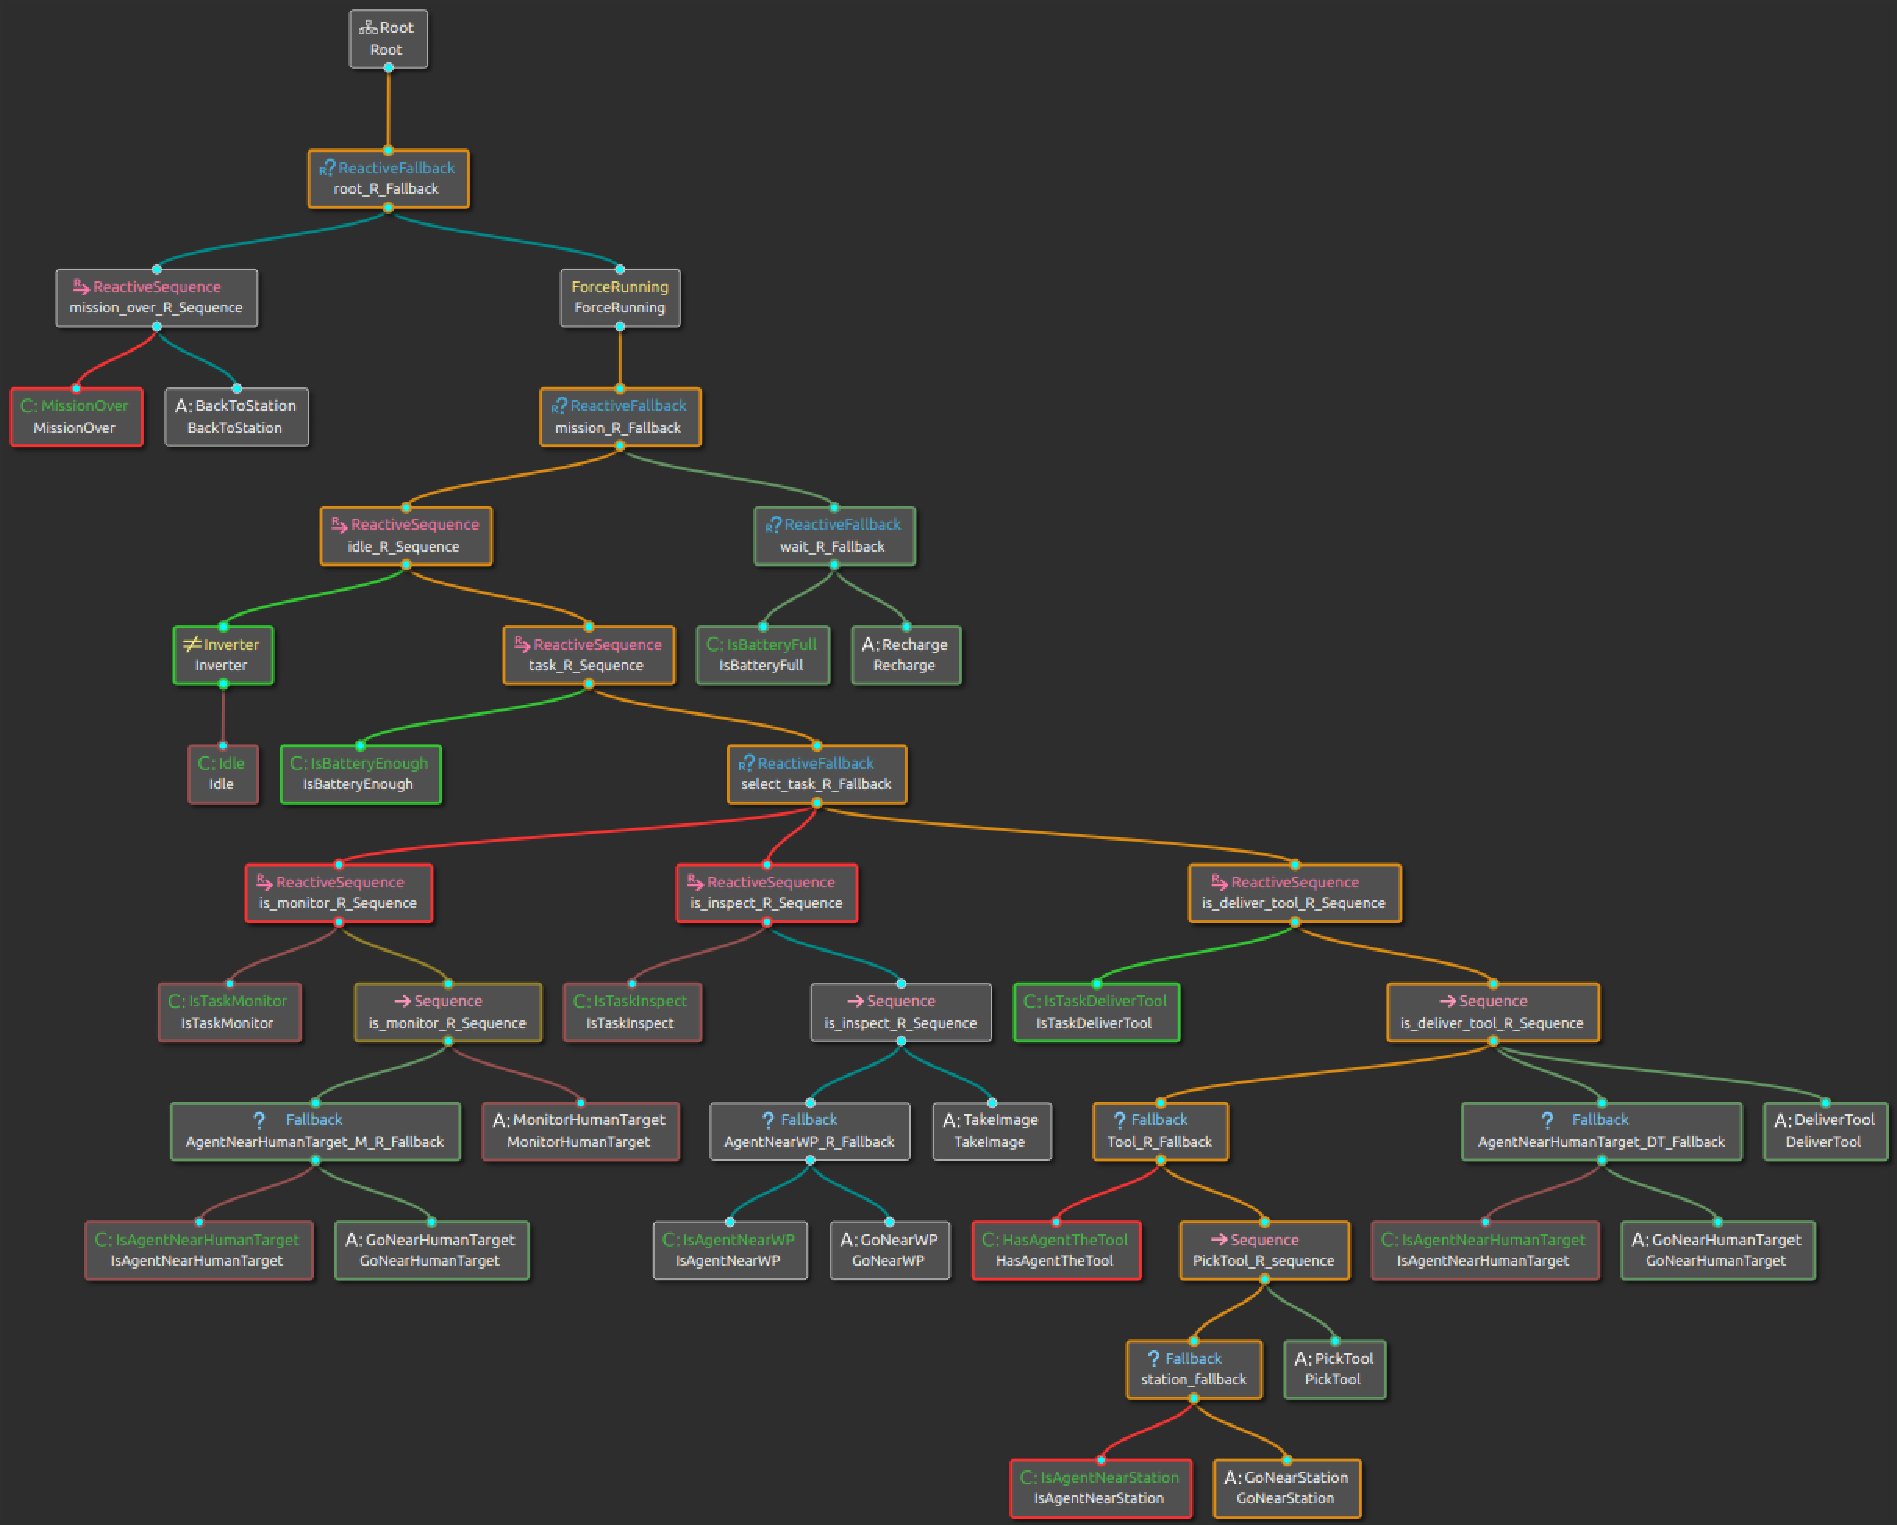
\includegraphics[width=.3\linewidth]{Results/figures/BTImprevistoMDT_3.pdf}}
    \caption{Evolution of the \gls{BT} during a change of plans. \emph{Tool Delivery} task displaces \emph{Safety Monitoring} task}
    \label{fig:event_ChangeOfPlans}
\end{figure}

After the success of the previous test, it was tested whether the \emph{High-Level Planner} is able to handle the situation when a new task with a repeated \gls{ID} arrives. For this purpose, an \emph{Inspection} task with the same \gls{ID} as the previous \emph{Tool Delivery} task was sent before the previous \emph{Tool Delivery} task was finished. The system passed the test successfully as shown in code \ref{exit:event_DuplicatedID}, the task was cancelled and deleted by the \emph{High-Level Planner} and the \gls{BT}, who halted the previous task and completed the new one successfully, remaining at the end executing the monitoring task requested at the beginning of the simulation, which has not yet finished. As the \gls{BT} simply reacted to the change of plans exactly as in the previous situation, no figure is now displayed.

\begin{lstlisting}[caption={Feedback messages printed after the arrival of a task with a repeated id. \emph{Inspection} task overwrites \emph{Tool Delivery} task}, breaklines=true, label=exit:event_DuplicatedID]
    [ WARN][/task_planner]: [incomingTask] Duplicated ID. An unfinished task is going to be deleted: task_4(DeliverTool)
    [ INFO][/task_planner]: [incomingTask] Received a New Task:
        task_4: Inspect
            Positions: (0, 0, 2) (10, 10, 2) (0, 10, 2) (10, 0, 2)
            Agent List:
    
    [ INFO][/task_planner]: [incomingTask] Allocating tasks...
    [ INFO][/task_planner]: [performTaskAllocation] Tasks Allocated:
    [ INFO][/task_planner]: [performTaskAllocation] Agent id: uav_1
        Agent type: PhysicalACW
        Task list: (2 tasks)
            task_4: Inspect
            task_3: Monitor
    
    [ INFO][/uav_1/agent]: [newTaskList] Received a NewTaskList Action
    [ INFO][/uav_1/agent]: task_4: Inspect
    [ INFO][/uav_1/agent]: [PickTool] halt requested
    [ INFO][/uav_1/agent]: [PickTool] PICK TOOL FINISHED
    [ INFO][/uav_1/agent]: [GoNearWP] Moving near WP...
    [ INFO][/uav_1/agent]: [TakeImage] Calling Lower-level controllers...
    [ INFO][/uav_1/agent]: [TakeImage] INSPECT TASK FINISHED (true)
    [ INFO][/task_planner]: [taskResultCB] (uav_1) task_4(Inspect) SUCCEEDED. Reallocating just in case...
    [ INFO][/uav_1/agent]: task_3: Monitor
    [ INFO][/uav_1/agent]: [GoNearHumanTarget] Moving near HT...
    [ INFO][/uav_1/agent]: [MonitorHumanTarget] Calling Lower-level controllers...
\end{lstlisting}

Next, the battery level was suddenly lowered to check the \gls{BT}'s reaction. The \gls{BT} immediately stopped the execution of the task to make an emergency visit to the charging station as shown in the figure \ref{fig:event_battery}. Note that the halt is not produced by \emph{Is Battery Enough} condition node, but by the emptying of the task queue as established by the protocol. Thus, the node that stops the execution of the task should always be \emph{Idle}'s \emph{Inverter} node, not \emph{Is Battery Enough} condition node, which is there to provide the \gls{BT} with additional robustness in case of failure. It can also be seen in the feedback showed in code \ref{exit:event_battery} that the \emph{Agent Behaviour Manager} communicated to the \emph{High-Level Planner} the detection of the unforeseen event, which triggered a replanning on its side. Note that this test was possible thanks to the functions programmed in the block in charge of faking the \gls{UAV}'s battery.

\begin{figure}[htbp]
    \centering
    \subfloat[\emph{Safety Monitoring} tree running]{
        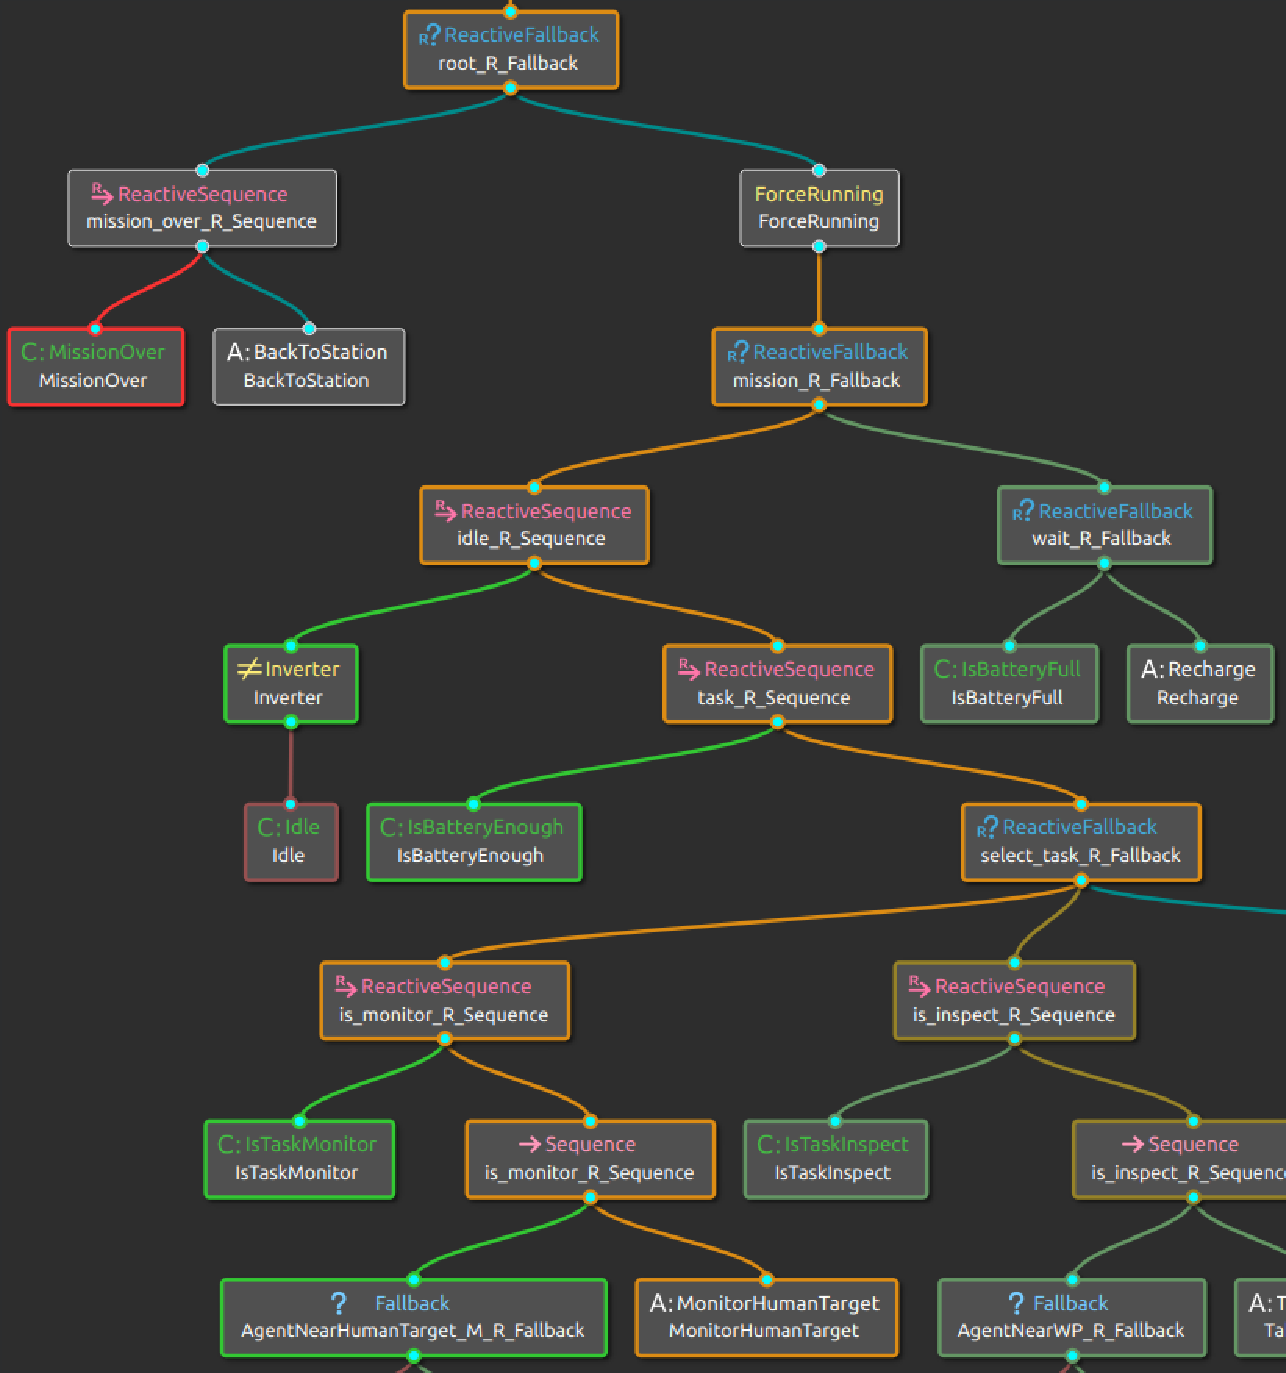
\includegraphics[width=.3\linewidth]{Results/figures/BTImprevistoBat_1.pdf}}
    \hfill
    \subfloat[\emph{Safety Monitoring} tree is halted becouse \emph{Idle}'s \emph{Inverter} node returns \emph{FAILURE}]{
        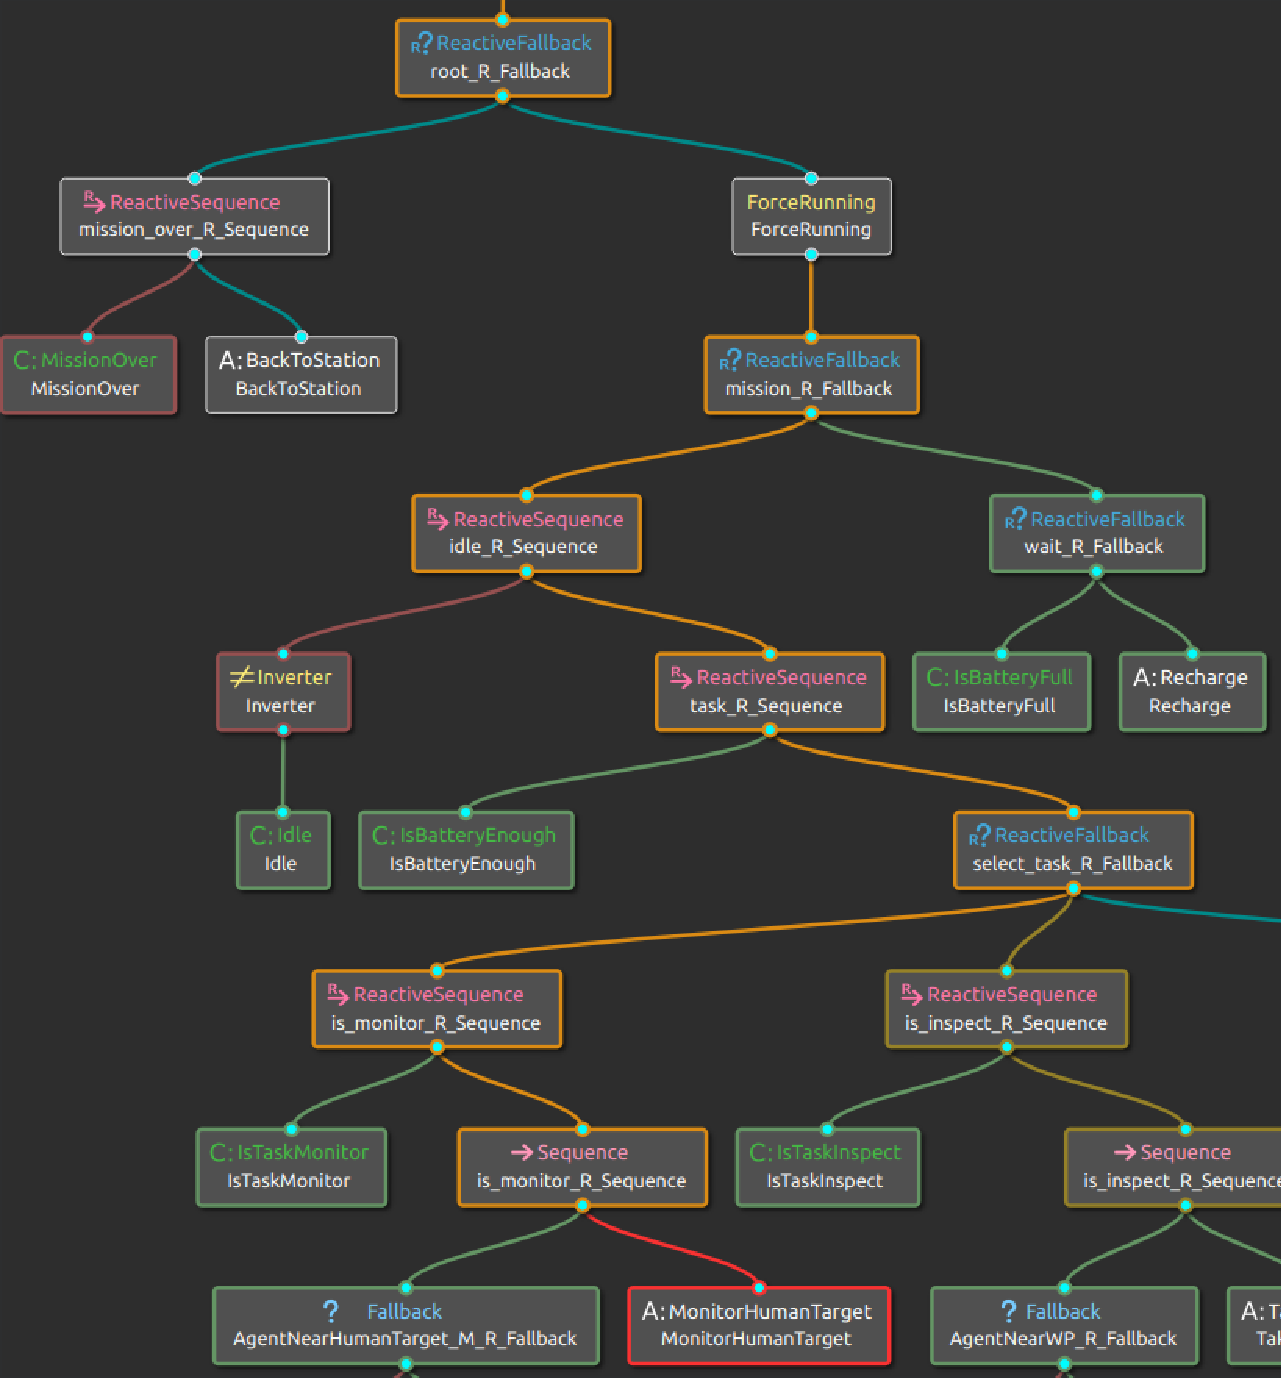
\includegraphics[width=.3\linewidth]{Results/figures/BTImprevistoBat_2.pdf}}
    \hfill
    \subfloat[\emph{Recharge} node running]{
        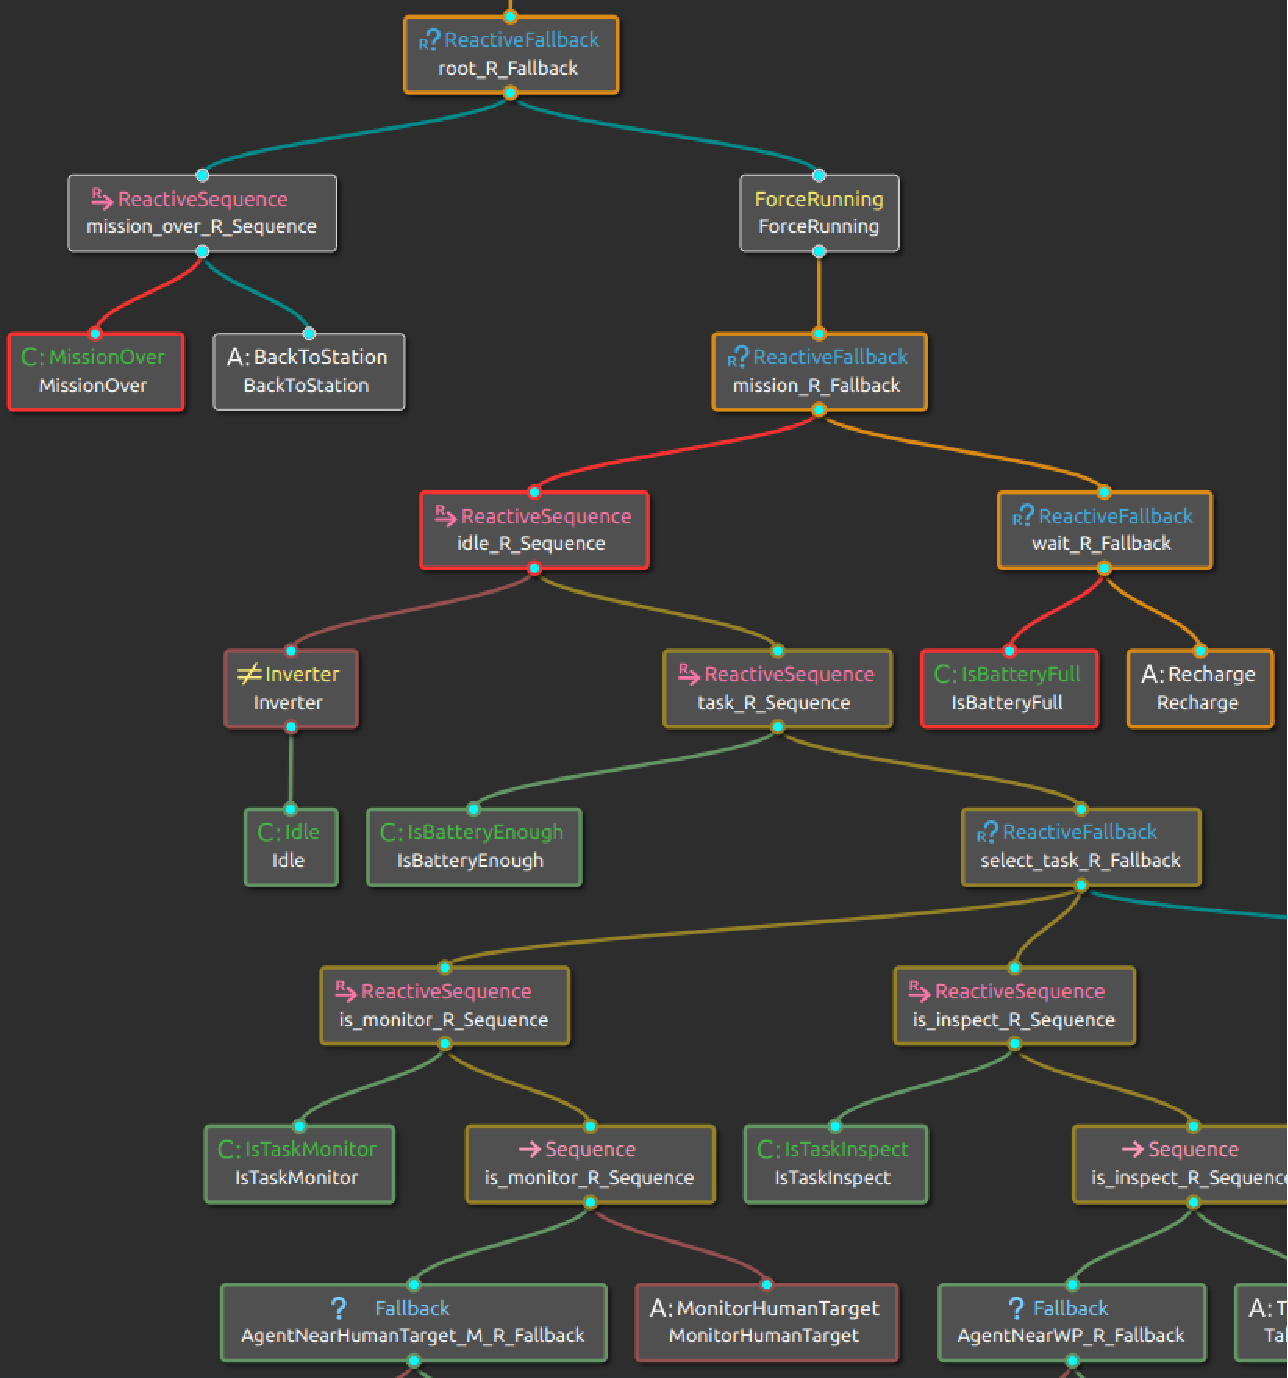
\includegraphics[width=.3\linewidth]{Results/figures/BTImprevistoBat_3.pdf}}
    \caption{Emergency protocol in the event of an insufficient battery}
    \label{fig:event_battery}
\end{figure}

\begin{lstlisting}[caption={Feedback messages printed after insufficient battery event}, breaklines=true, label=exit:event_battery]
    [ WARN][/uav_1/agent]: [isBatteryEnough] Advertising that battery_enough_ = false
    [ INFO][/uav_1/agent]: [MonitorHumanTarget] halt requested
    [ INFO][/uav_1/agent]: [MonitorHumanTarget] MONITOR TASK FINISHED (false)
    [ INFO][/uav_1/agent]: [Recharge] Calling take_off
    [ INFO][/uav_1/agent]: [Recharge] Moving to recharging station
    [ INFO][/uav_1/agent]: [Recharge] Calling land
    [ INFO][/uav_1/agent]: [Recharge] Charging...
    
    [ WARN][/task_planner]: [batteryEnoughCB] (uav_1) Noticed that battery_enough_ = false
    [ INFO][/task_planner]: [performTaskAllocation] Tasks Allocated:
    [ INFO][/task_planner]: [performTaskAllocation] Agent id: uav_1
        Agent type: PhysicalACW
        Task list: (0 tasks)
    
    [ INFO][/uav_1/agent]: [newTaskList] Received a NewTaskList Action
\end{lstlisting}

At this point it is important to mention that a \emph{Recharge} task has not been implemented and therefore recharges cannot be planned as such, instead in the current solution the \emph{High-Level Planner} makes the \gls{ACW} recharge by not having any task queued. To make it stop recharging the planner only has to assign a task to it, either when the battery is full or before. Using the battery faker again, the battery was set to maximum and it was found that a new replanning took place and the \gls{BT} started the \gls{ACW} again (see code \ref{exit:event_batteryOK}). The evolution of the \gls{BT} is the same as shown in figures \ref{fig:BTinitialization} and \ref{fig:NoIdle_DeliverToolTaskTree} but with the difference that now the task is of the \emph{Safety Monitoring} type.

\begin{lstlisting}[caption={Feedback messages printed after enough battery event}, breaklines=true, label=exit:event_batteryOK]
    [ WARN][/uav_1/agent]: [isBatteryEnough] Advertising that battery_enough_ = true

    [ WARN][/task_planner]: [batteryEnoughCB] (uav_1) Noticed that battery_enough_ = true
    [ INFO][/task_planner]: [performTaskAllocation] Tasks Allocated:
    [ INFO][/task_planner]: [performTaskAllocation] Agent id: uav_1
        Agent type: PhysicalACW
        Task list: (1 tasks)
            task_3: Monitor
    
    [ INFO][/uav_1/agent]: [newTaskList] Received a NewTaskList Action
    [ INFO][/uav_1/agent]: task_3: Monitor
    [ INFO][/uav_1/agent]: [Recharge] halt requested
    [ INFO][/uav_1/agent]: [GoNearHumanTarget] Moving near HT...
    [ INFO][/uav_1/agent]: [MonitorHumanTarget] Calling Lower-level controllers...
\end{lstlisting}

The other possible emergency situation is the loss of connection between the two blocks that make up this work. To test this case the process that was running the \emph{High-Level Planner} was killed. The emergency situation was successfully detected by the \gls{BT} after the maximum timeout time had elapsed, after which the emergency protocol was activated and the \gls{ACW} was directed to the charging station. As the emergency protocol is the same, the evolution of the \gls{BT} in this scenario is the same as shown in figure \ref{fig:event_battery}. Code \ref{exit:event_AgentConnection} displays the feedback messages that are printed by the \emph{Agent Behavior Manager} block.

\begin{lstlisting}[caption={Feedback messages printed by the \emph{Agent Behavior Manager} block after a connection loss}, breaklines=true, label=exit:event_AgentConnection]
    [ WARN][/task_planner]: Shutdown request received.
    [ WARN][/task_planner]: Reason given for shutdown: [user request]
    
    [ WARN][/uav_1/agent]: [checkBeaconTimeout] Beacon timeout. Disconnection detected. Emptying the task queue.
    [ INFO][/uav_1/agent]: [MonitorHumanTarget] halt requested
    [ INFO][/uav_1/agent]: [MonitorHumanTarget] MONITOR TASK FINISHED (false)
    [ INFO][/uav_1/agent]: [Recharge] Calling take_off
    [ INFO][/uav_1/agent]: [Recharge] Moving to recharging station
    [ INFO][/uav_1/agent]: [Recharge] Calling land
    [ INFO][/uav_1/agent]: [Recharge] Charging...
\end{lstlisting}

Finally, in a new simulation, during a \emph{Safety Monitoring} task, the \emph{Mission Over} signal was sent to observe the completion of both blocks. The \emph{Agent Behaviour Manager} directed the \gls{ACW} to the base station and then the \gls{BT} and the entire block were terminated (see Fig. \ref{fig:event_MissionOver}). The \emph{High-Level Planner}, after detecting the signal, waited for all \glspl{ACW} to finish and then shut down as well (see code \ref{exit:event_MissionOver}).

% \ref{fig:event_MissionOver} Groot y terminal del proceso de mission over
\begin{figure}[htbp]
    \centering
    \subfloat[\emph{Safety Monitoring} tree running]{
        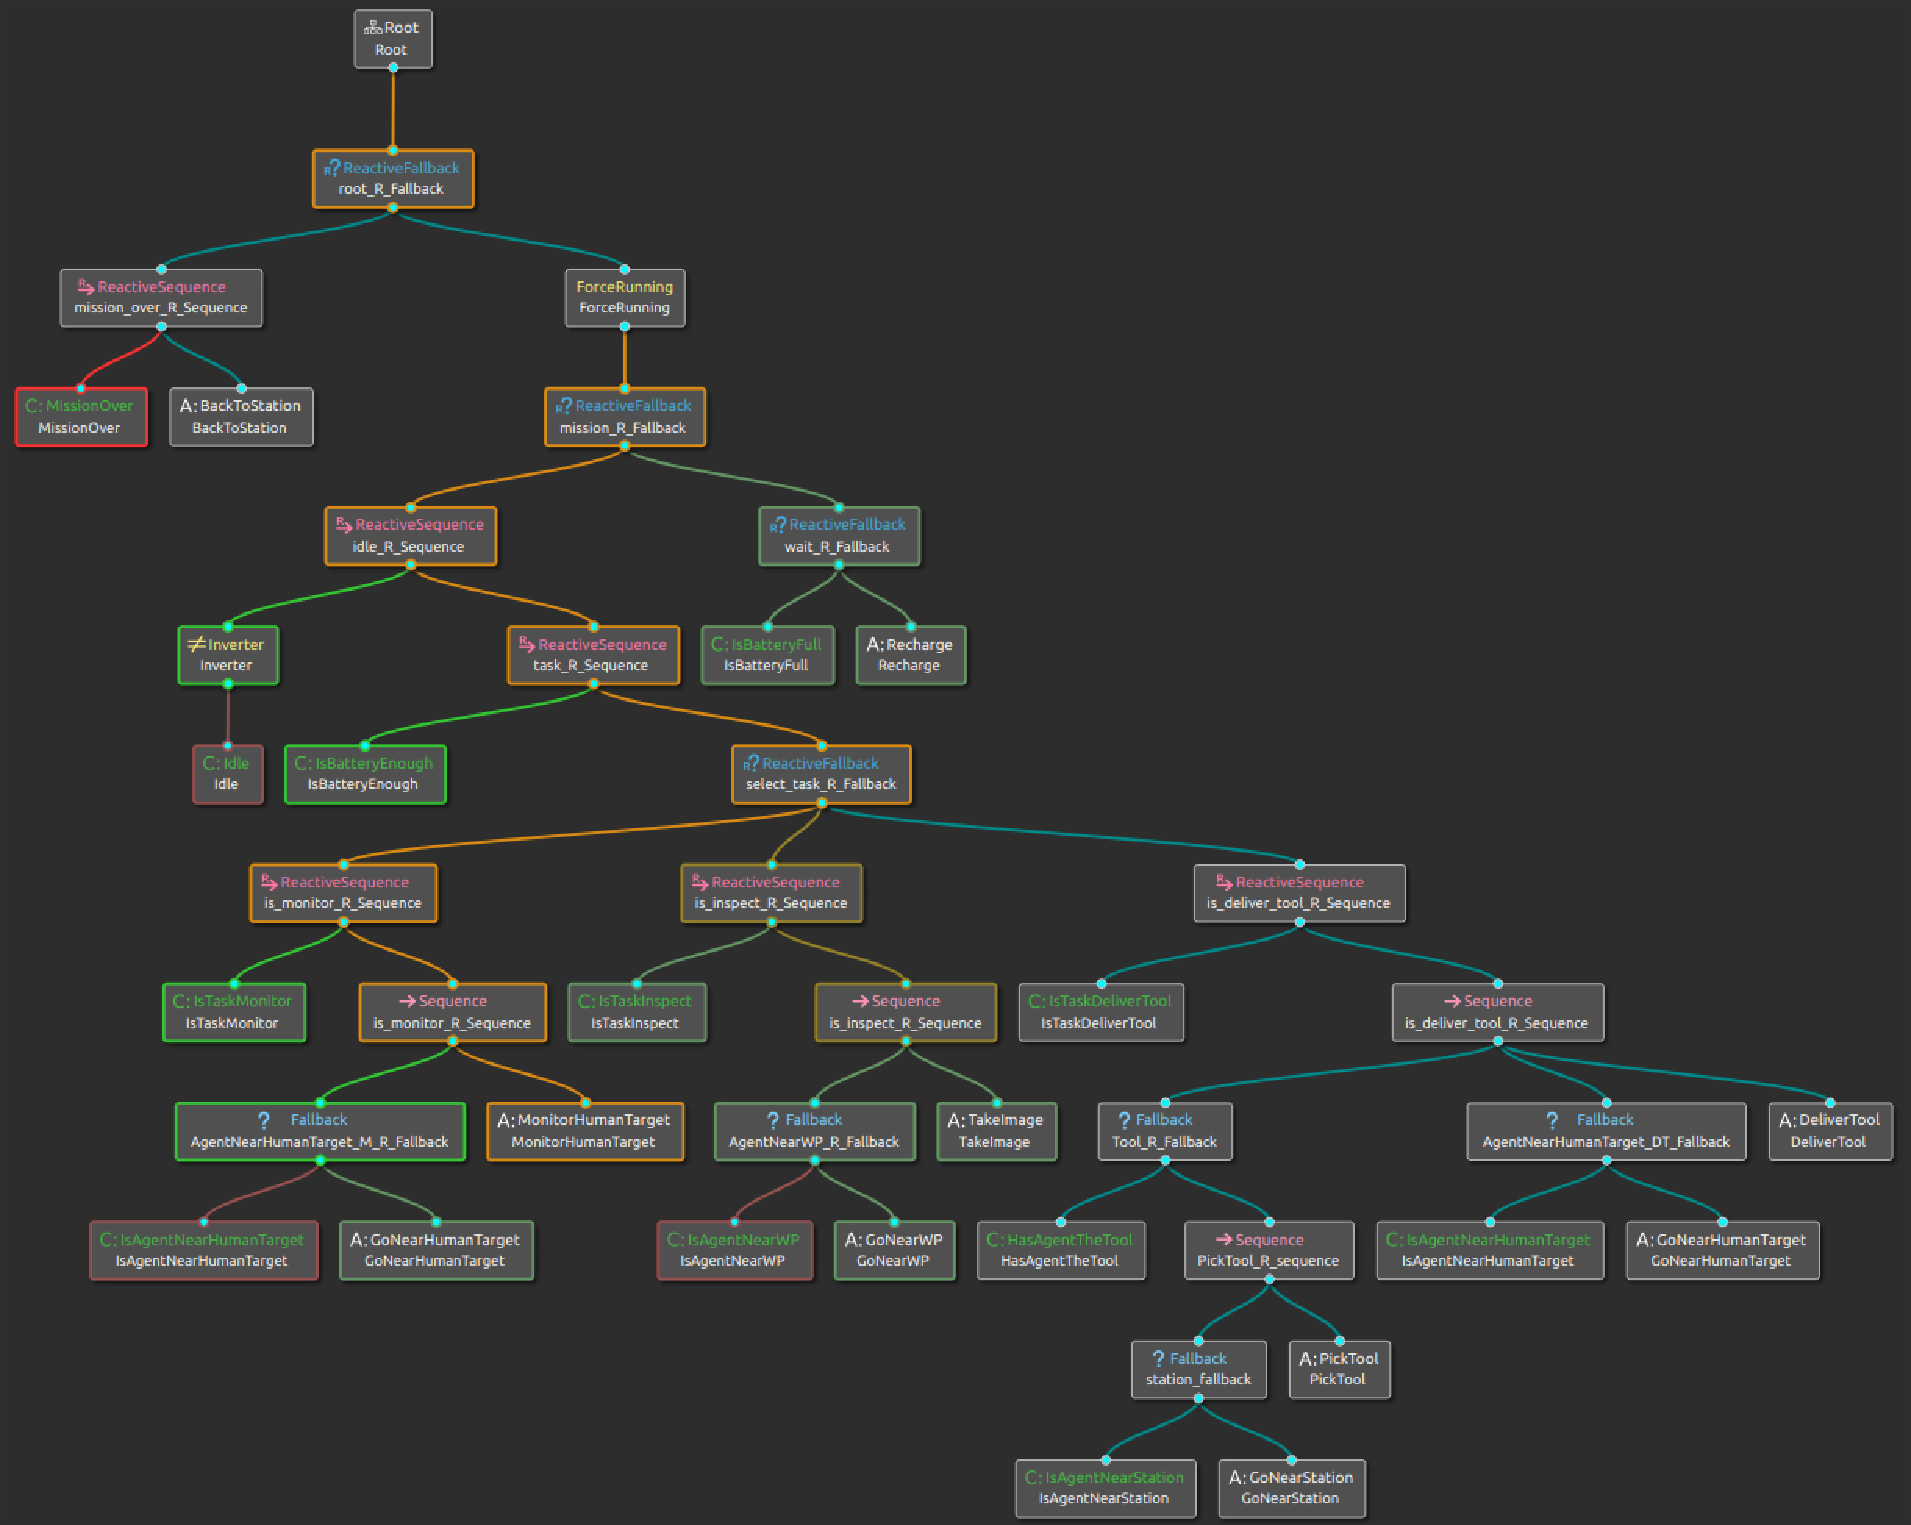
\includegraphics[width=.45\linewidth]{Results/figures/BTMO_1.pdf}}
    \hfill
    \subfloat[\emph{Safety Monitoring} tree is halted becouse \emph{Mission Over} condition is true. \emph{Back to Station} node running]{
        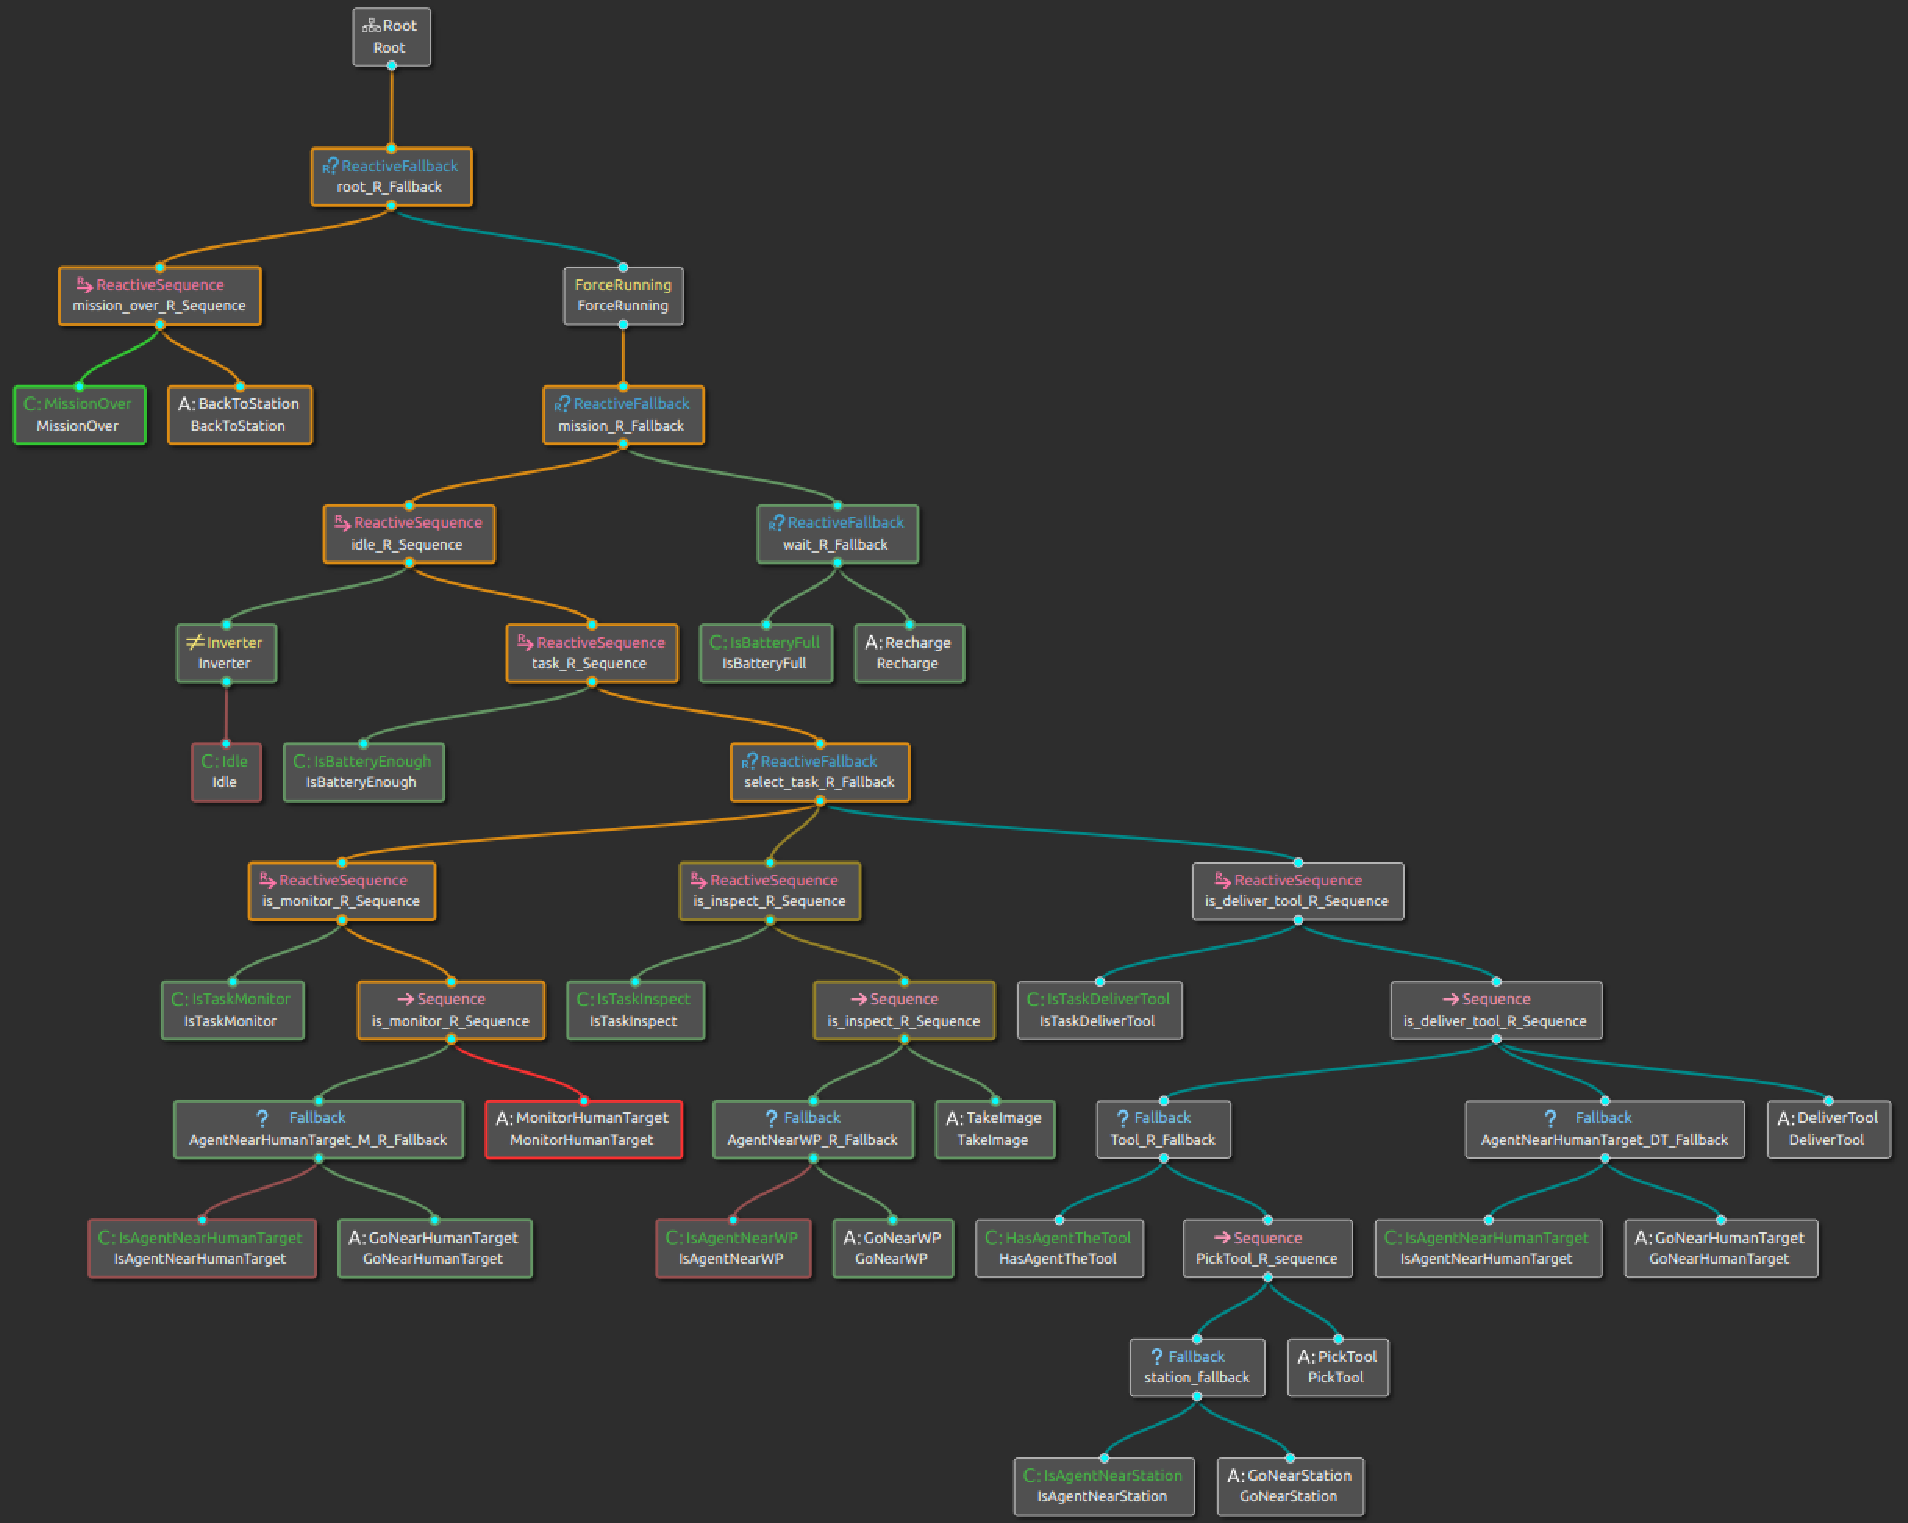
\includegraphics[width=.45\linewidth]{Results/figures/BTMO_2.pdf}}
    \\
    \subfloat[\emph{Back to Station} node returns \emph{SUCCESS} so \gls{BT}'s root does the same]{
        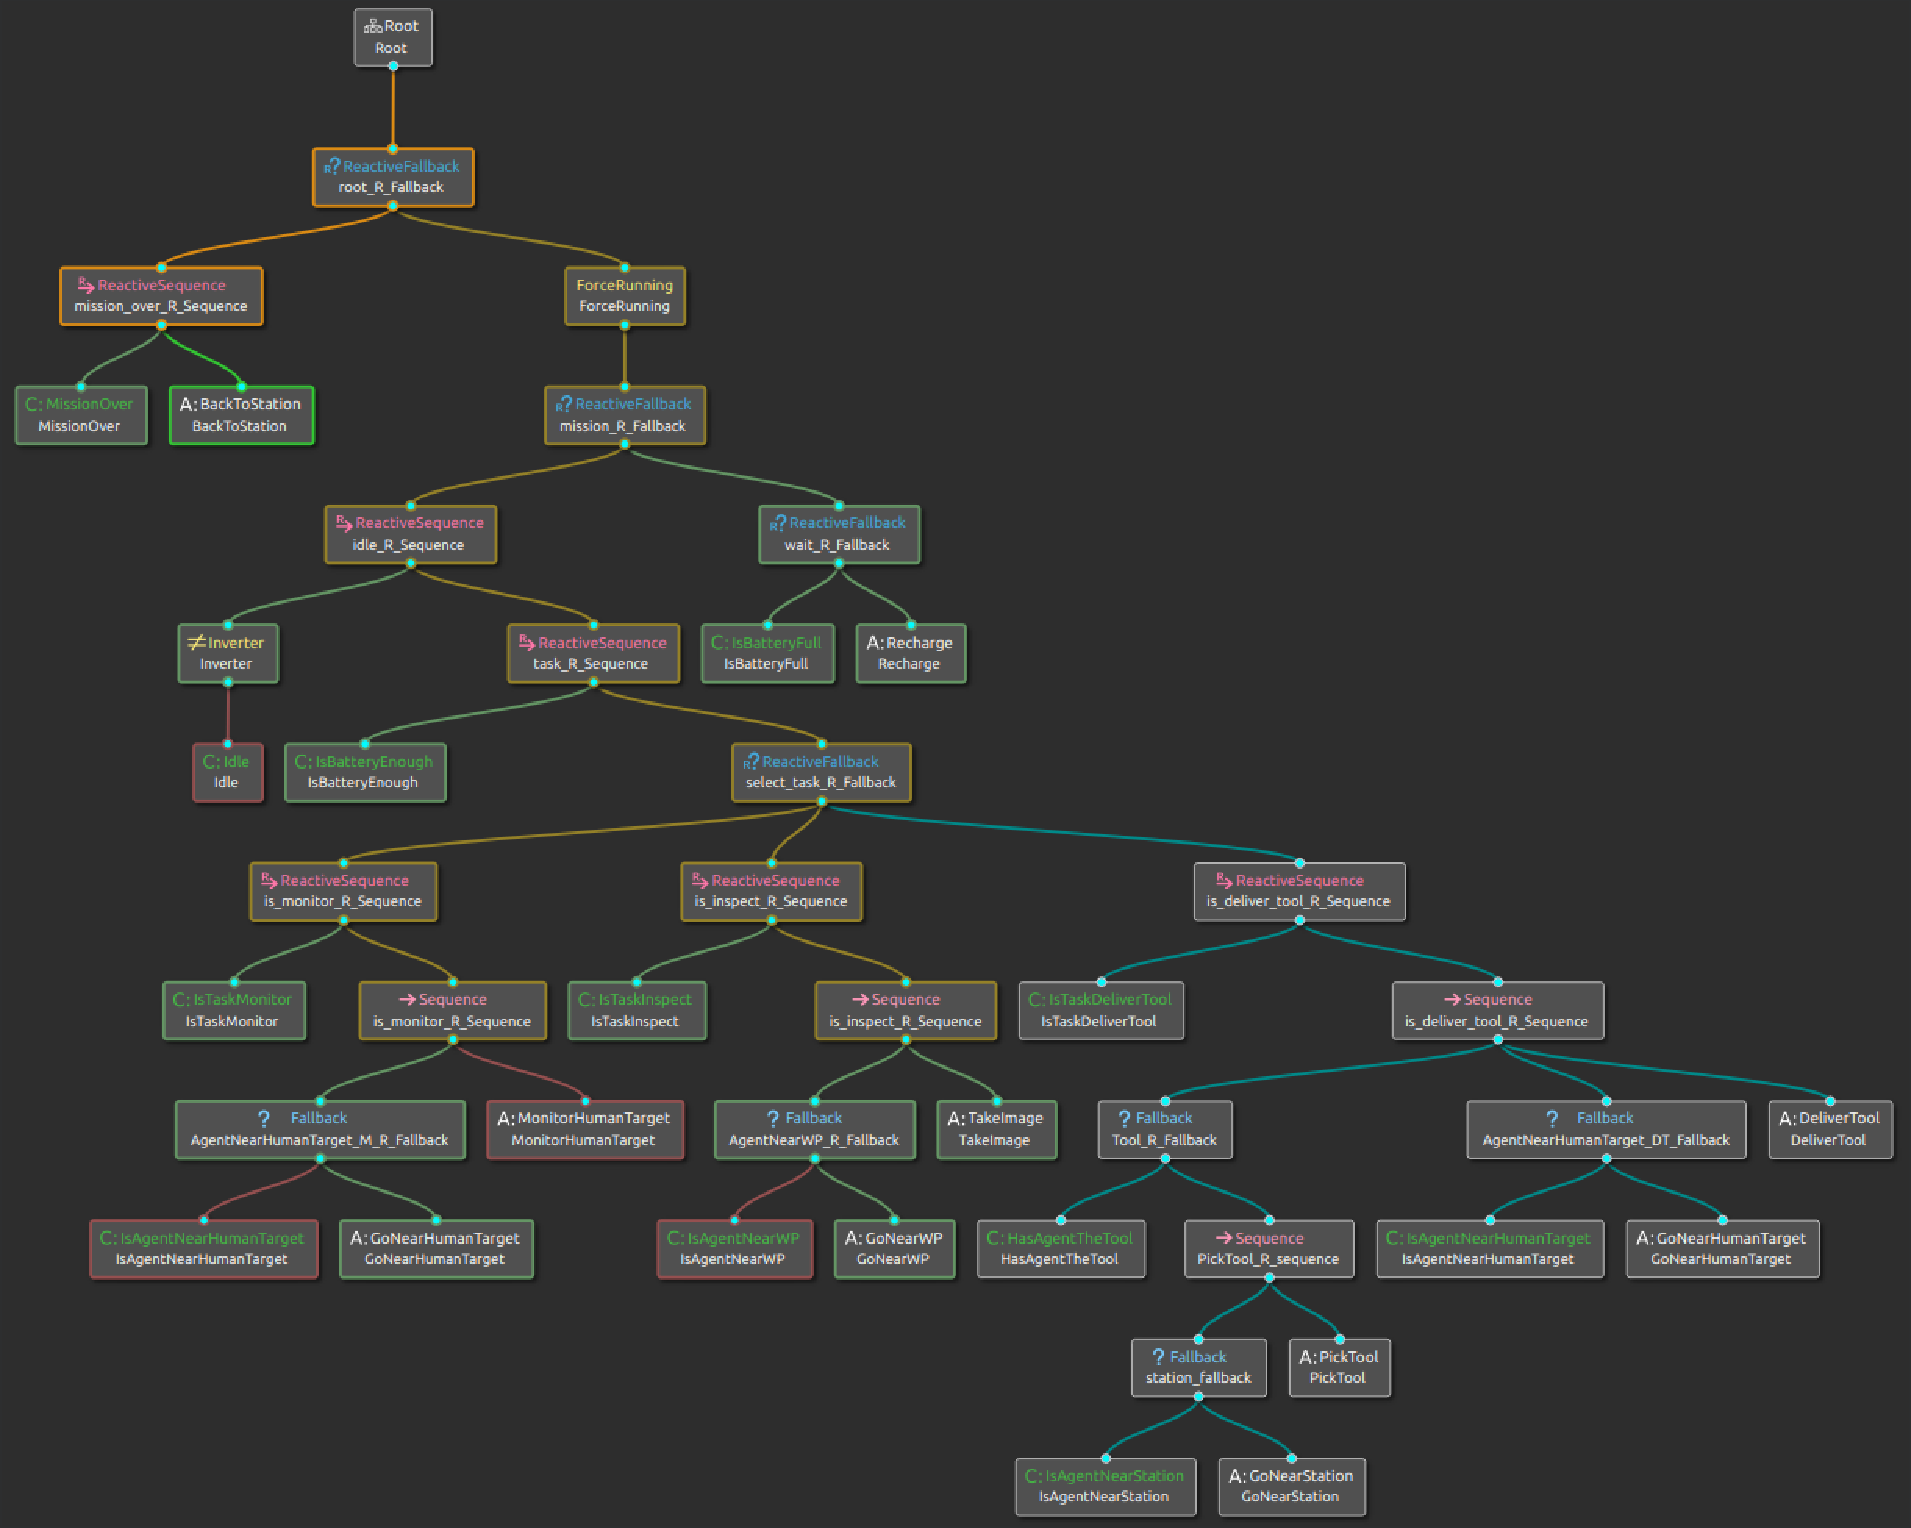
\includegraphics[width=.45\linewidth]{Results/figures/BTMO_3.pdf}}
        \hfill
    \subfloat[\emph{Agent Behaviour Manager} block exits the main while and \gls{BT} is powered off]{
        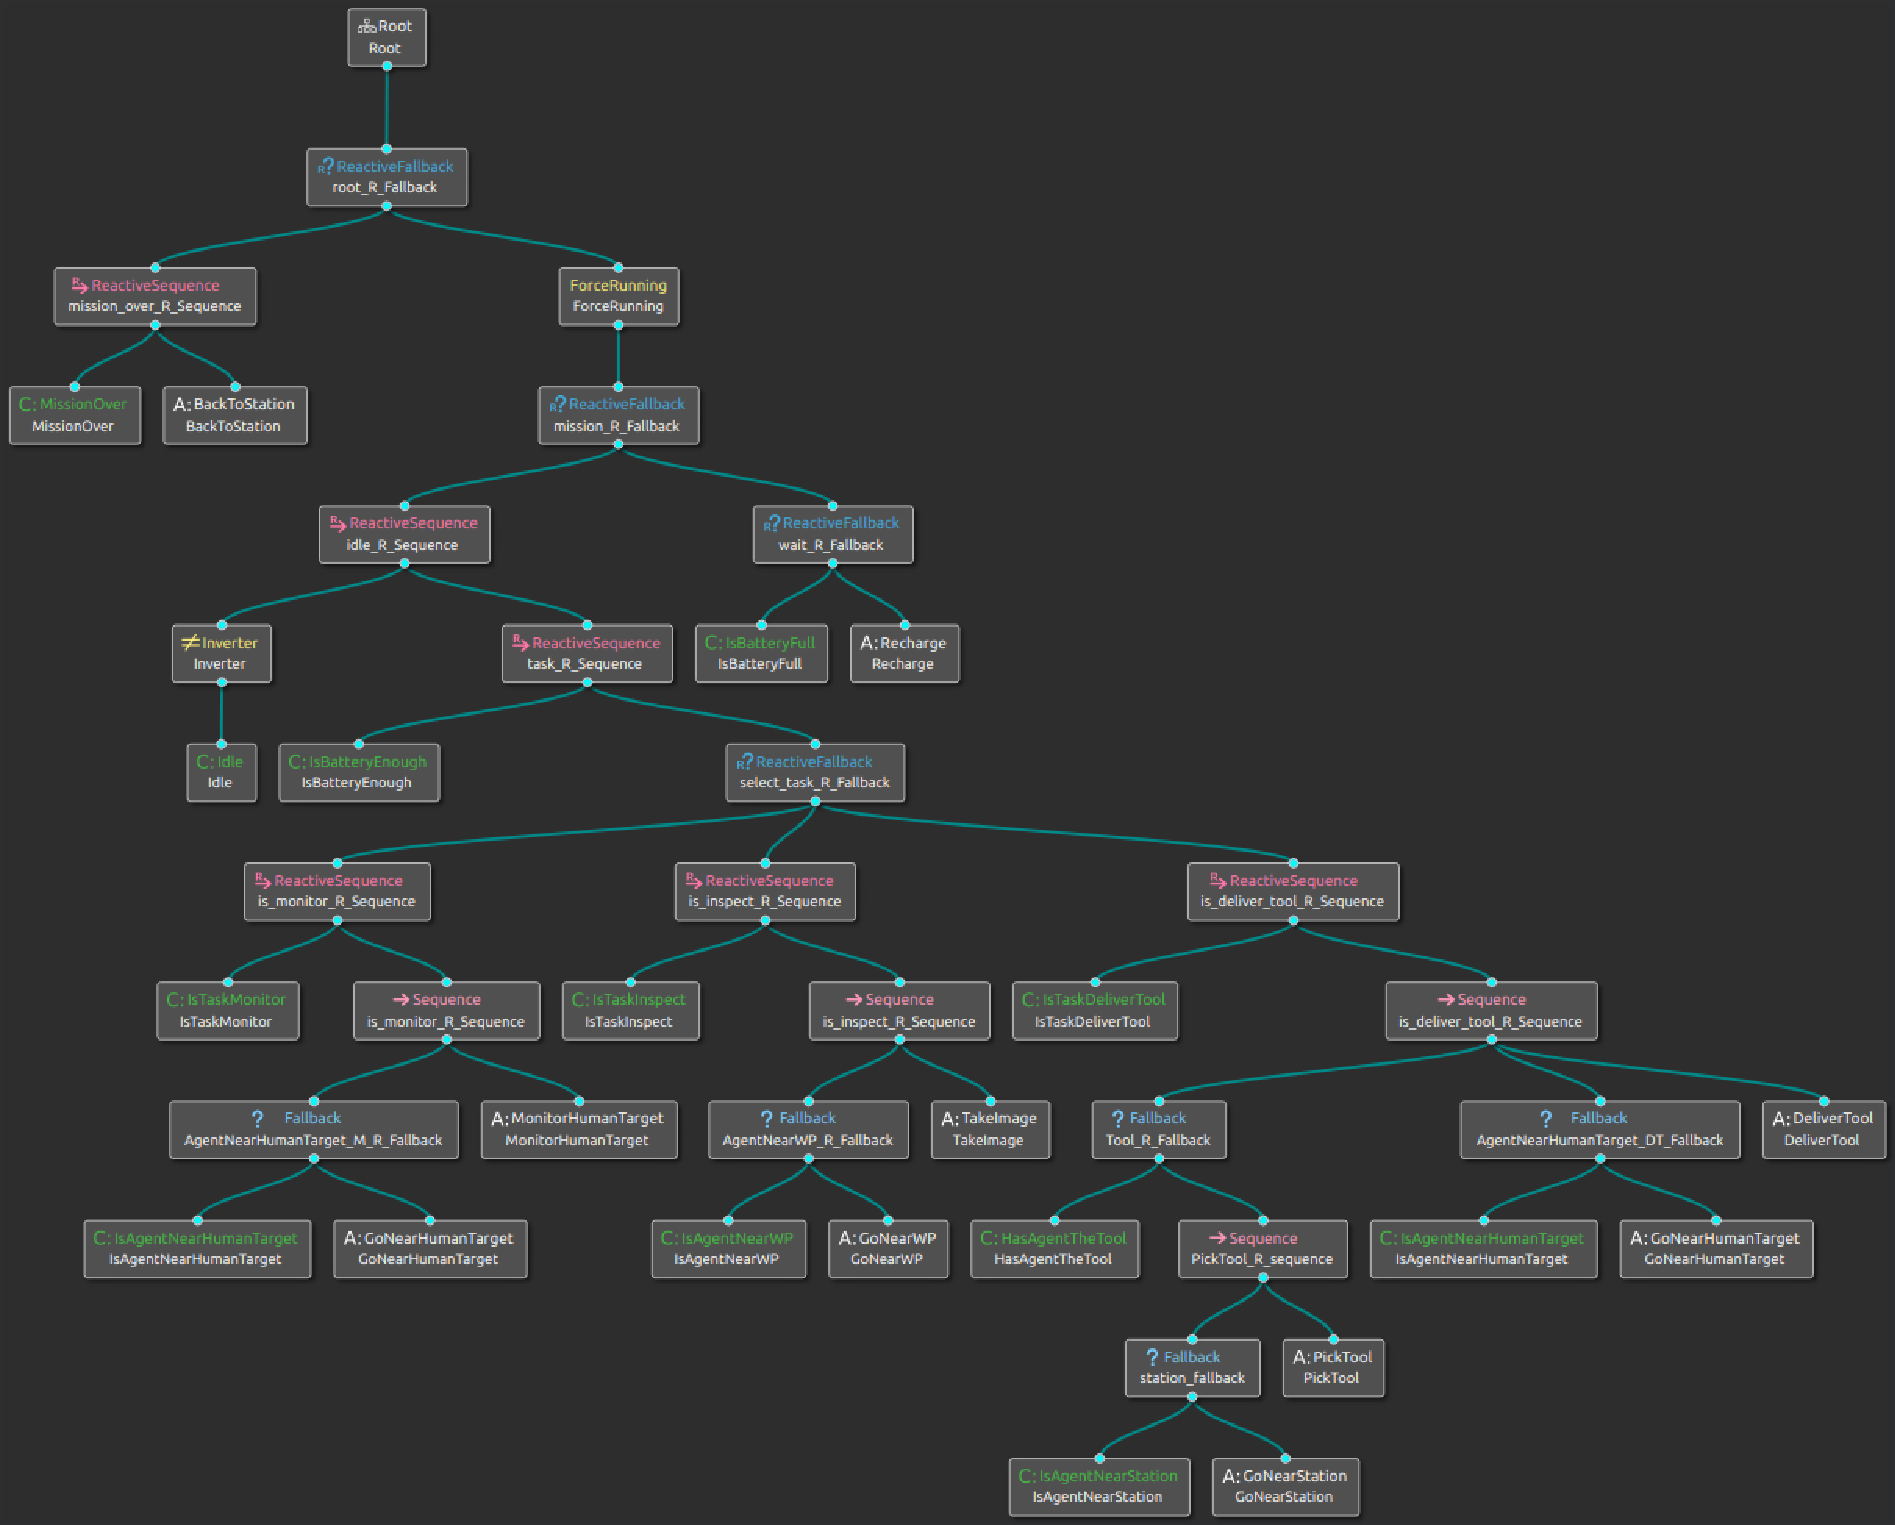
\includegraphics[width=.45\linewidth]{Results/figures/BTMO_4.pdf}}
    \caption{\gls{BT} leading \gls{ACW} to station and shutting down after the arrival of a mission over signal}
    \label{fig:event_MissionOver}
\end{figure}

\begin{lstlisting}[caption={Feedback messages printed after mission over signal}, breaklines=true, label=exit:event_MissionOver]
    [ INFO][/task_planner]: [Planner] Mission Over. Waiting for the agents to finish

    [ INFO][/uav_1/agent]: [MonitorHumanTarget] halt requested
    [ INFO][/uav_1/agent]: [MonitorHumanTarget] MONITOR TASK FINISHED (false)
    [ INFO][/uav_1/agent]: [BackToStation] Emptying the Queue...
    [ INFO][/uav_1/agent]: [BackToStation] Calling take_off
    [ INFO][/uav_1/agent]: [BackToStation] Moving to station
    [ INFO][/uav_1/agent]: [BackToStation] Calling land

    [ INFO][/uav_1/agent]: [BackToStation] halt requested
    [ INFO][/uav_1/agent]: [GoNearHumanTarget] halt requested
    [ INFO][/uav_1/agent]: [MonitorHumanTarget] halt requested
    [ INFO][/uav_1/agent]: [GoNearWP] halt requested
    [ INFO][/uav_1/agent]: [TakeImage] halt requested
    [ INFO][/uav_1/agent]: [GoNearStation] halt requested
    [ INFO][/uav_1/agent]: [PickTool] halt requested
    [ INFO][/uav_1/agent]: [GoNearHumanTarget] halt requested
    [ INFO][/uav_1/agent]: [DeliverTool] halt requested
    [ INFO][/uav_1/agent]: [Recharge] halt requested

    [uav_1/agent-3] process has finished cleanly

    [ WARN][/task_planner]: [checkBeaconsTimeout] Beacon Timeout. uav_1 disconnected.
    [ INFO][/task_planner]: [main] Ending...
    
    [task_planner-2] process has finished cleanly
\end{lstlisting}

\section{Phase II: multi-ACW simulations}
\label{sec:phaseII}
The tests in this phase consisted of a simulation with five \glspl{ACW} including one \emph{Physical-ACW} (UAV\_1), one \emph{Inspection-ACW} (UAV\_2) and three \emph{Safety-ACWs} (UAV\_3, UAV\_4, UAV\_5). The tests were carried out in a single simulation, which was organised in such a way as to be sufficient to validate the \emph{High-Level Planner} under all circumstances.

% Llegan tareas y no hay ningún UAV connectado. Lista de tareas pendientes
% tareas_1:
	% @rosrun human_aware_collaboration_planner gesture_task task_1 D hammer human_target_2
	% @rosrun human_aware_collaboration_planner gesture_task task_2 I 0 0 2 10 10 2 0 10 2 10 0 2
	% @rosrun human_aware_collaboration_planner gesture_task task_3 M human_target_1 1.5 4
The first step was to start the simulation. Each \emph{Agent Behaviour Manager} was programmed to wait for ten seconds in order to allow time to send tasks while no \gls{ACW} was connected. The code \ref{exit:NoAgentsCoonectedYet} shows the feedback printed by the terminal up to that point. The function of the centralised module that carries out the task distribution communicated that no \glspl{UAV} were connected yet and postponed the planning.

\begin{lstlisting}[caption={Feedback messages printed after the start of the simulation before the ACWs were connected}, breaklines=true, label=exit:NoAgentsCoonectedYet]
    [ INFO][/task_planner]: [Planner] Initialization complete

    [ INFO][/task_planner]: [incomingTask] Received New Tasks:
	    task_1: Deliver
		    Tool: hammer (1.5kg): -2, 5, 0.9
		    Human Target: human_target_2: -5, 15, 1.8
	    task_2: Inspect
		    Positions: (0, 0, 2) (10, 10, 2) (0, 10, 2) (10, 0, 2)
		    Agent List:
	    task_3: Monitor (1.5, 4)
		    Human Target: human_target_1: 0, 10, 1.85
		    Agent List:

    [ INFO][/task_planner]: [incomingTask] Allocating tasks...
    [ WARN][/task_planner]: [performTaskAllocation] No Agents connected yet. 3 pending tasks
\end{lstlisting}

After the ten seconds had elapsed, while the communication between the \emph{High-Level Planner} and the \emph{Agent Behaviour Managers} was established and the first block was calculating the mission plan, the \glspl{BT} guided the \glspl{ACW} to the charging station as stipulated when there is an empty queue (see code \ref{exit:IdleCharging}).

\begin{lstlisting}[caption={Feedback messages printed before the \glspl{ACW} received their new queues}, breaklines=true, label=exit:IdleCharging]
    [ INFO][/uav_1/agent]: [AgentNode] uav_1 initialized.
    [ INFO][/uav_1/agent]: [Recharge] Calling take_off
    [ INFO][/uav_1/agent]: [Recharge] Moving to recharging station
    [ INFO][/uav_1/agent]: [Recharge] Calling land
    [ INFO][/uav_1/agent]: [Recharge] Charging...
    
    [ INFO][/uav_2/agent]: [AgentNode] uav_2 initialized.
    [ INFO][/uav_2/agent]: [Recharge] Calling take_off
    [ INFO][/uav_2/agent]: [Recharge] Moving to recharging station
    [ INFO][/uav_2/agent]: [Recharge] Calling land
    [ INFO][/uav_2/agent]: [Recharge] Charging...
    
    [ INFO][/uav_3/agent]: [AgentNode] uav_3 initialized.
    [ INFO][/uav_3/agent]: [Recharge] Calling take_off
    [ INFO][/uav_3/agent]: [Recharge] Moving to recharging station
    [ INFO][/uav_3/agent]: [Recharge] Calling land
    [ INFO][/uav_3/agent]: [Recharge] Charging...
    
    [ INFO][/uav_4/agent]: [AgentNode] uav_4 initialized.
    [ INFO][/uav_4/agent]: [Recharge] Calling take_off
    [ INFO][/uav_4/agent]: [Recharge] Moving to recharging station
    [ INFO][/uav_4/agent]: [Recharge] Calling land
    [ INFO][/uav_4/agent]: [Recharge] Charging...

    [ INFO][/uav_5/agent]: [AgentNode] uav_5 initialized.
    [ INFO][/uav_5/agent]: [Recharge] Calling take_off
    [ INFO][/uav_5/agent]: [Recharge] Moving to recharging station
    [ INFO][/uav_5/agent]: [Recharge] Calling land
    [ INFO][/uav_5/agent]: [Recharge] Charging...
\end{lstlisting}

Once the communication was established and the connection of the five \glspl{ACW} was detected, the \emph{High-Level Planner} executed a task allocation. The tasks pending at this point were a \emph{Tool Delivery} task, for which only one \gls{ACW} was capable (UAV\_1), an \emph{Inspection} task, which could be executed by all the connected \glspl{ACW}, but only one of them was of the preferred type (UAV\_2), and a \emph{Safety Monitoring} task that required four \glspl{ACW}, which could be executed by all of them but only three of them were of the preferred type. The code \ref{exit:FirstAllocation} shows the feedback that was printed on the screen after the connection of the \glspl{UAV} and the result of the planning.

\begin{lstlisting}[caption={Feedback messages printed after the connection of the \glspl{UAV} and the planning}, breaklines=true, label=exit:FirstAllocation]
    [ INFO][/task_planner]: [beaconCallback] New Agent connected: uav_1
    [ INFO][/task_planner]: [beaconCallback] New Agent connected: uav_2
    [ INFO][/task_planner]: [beaconCallback] New Agent connected: uav_3
    [ INFO][/task_planner]: [beaconCallback] New Agent connected: uav_4
    [ INFO][/task_planner]: [beaconCallback] New Agent connected: uav_5
    
    [ INFO][/task_planner]: [performTaskAllocation] Tasks Allocated:
    
    [ INFO][/task_planner]: [performTaskAllocation] Agent id: uav_1
        Agent type: PhysicalACW
        Task list: (1 tasks)
            task_1: DeliverTool
    
    [ INFO][/task_planner]: [performTaskAllocation] Agent id: uav_2
    Agent type: InspectionACW
        Task list: (2 tasks)
            task_2: Inspect
            task_3: Monitor
    
    [ INFO][/task_planner]: [performTaskAllocation] Agent id: uav_3
        Agent type: SafetyACW
        Task list: (1 tasks)
            task_3: Monitor
    
    [ INFO][/task_planner]: [performTaskAllocation] Agent id: uav_4
        Agent type: SafetyACW
        Task list: (1 tasks)
            task_3: Monitor
    
    [ INFO][/task_planner]: [performTaskAllocation] Agent id: uav_5
        Agent type: SafetyACW
        Task list: (1 tasks)
            task_3: Monitor
\end{lstlisting}

% Asignación de las tareas: elección de parámetros, elección de los UAV, como quedan las colas finalmente.
The outcome of the mission planning was as expected. The highest priority task was assigned to the only \gls{ACW} capable of carrying it out, UAV\_1. The second highest priority task could be assigned by decision of the \emph{High-Level Planner} to more than one \gls{ACW}. It was assigned to a single \gls{ACW}, UAV\_2, which was the only \gls{UAV} of the preferred \gls{ACW} type for this task. Finally, the four \glspl{ACW} selected for the \emph{Safety Monitoring} task were UAV\_2, UAV\_3, UAV\_4 and UAV\_5, three of which were of the preferred type for this task, as they were still free at this point and also this way no \gls{ACW} qualified for another task is occupied. This task was to be started with only three \glspl{ACW} even though four were requested, as there were no more \glspl{ACW} available at that time. The last \gls{ACW} selected was the \emph{Inspection-ACW}, which on the one hand would be the first \gls{ACW} that would be available to execute the task, and on the other hand, it had a lower cost for this task than the \emph{Physical-ACW}, since the latter is the only one capable of executing \emph{Tool Delivery} tasks and it is preferable not to have it busy doing a lower priority task in case a task of this type arrives.

% Ejecución de los planes
Once the queues were communicated to the \glspl{ACW}, they proceeded with the execution of the first task of their respective queues. Code \ref{exit:ExecutionFirstPlan} shows the messages printed by the \emph{Agent Behaviour Manager} blocks during the execution of the entire plan. Note that when an \gls{UAV} completes all its assigned tasks, it returns to the station to recharge the battery while waiting. These messages were printed from the \gls{BT} nodes, being sufficient to know the status of each one of them.  No screenshots of the \glspl{BT} are shown at this stage because they have already been validated and these messages are enough.

\begin{lstlisting}[caption={Feedback messages printed by the \emph{Agent Behaviour Managers} during the plan execution}, breaklines=true, label=exit:ExecutionFirstPlan]
    [ INFO][/uav_1/agent]: [newTaskList] Received a NewTaskList Action
    [ INFO][/uav_1/agent]: task_1: DeliverTool
    [ INFO][/uav_1/agent]: [Recharge] halt requested
    [ INFO][/uav_1/agent]: [GoNearStation] Moving near Tool...
    [ INFO][/uav_1/agent]: [PickTool] Calling Lower-level controllers...
    [ INFO][/uav_1/agent]: [PickTool] PICK TOOL FINISHED
    [ INFO][/uav_1/agent]: [GoNearHumanTarget] Moving near HT...
    [ INFO][/uav_1/agent]: [DeliverTool] Calling Lower-level controllers...
    [ INFO][/uav_1/agent]: [DeliverTool] DELIVER TOOL TASK FINISHED (true)
    [ INFO][/task_planner]: [taskResultCB] task_1(DeliverTool) SUCCEEDED. Reallocating just in case...
    [ INFO][/uav_1/agent]: [Recharge] Moving to recharging station
    [ INFO][/uav_1/agent]: [Recharge] Calling land
    [ INFO][/uav_1/agent]: [Recharge] Charging...
    
    [ INFO][/uav_2/agent]: [newTaskList] Received a NewTaskList Action
    [ INFO][/uav_2/agent]: task_2: Inspect
    [ INFO][/uav_2/agent]: [Recharge] halt requested
    [ INFO][/uav_2/agent]: [GoNearWP] Moving near WP...
    [ INFO][/uav_2/agent]: [TakeImage] Calling Lower-level controllers...
    [ INFO][/uav_2/agent]: [TakeImage] INSPECT TASK FINISHED (true)
    [ INFO][/task_planner]: [taskResultCB] task_2(Inspect) SUCCEEDED. Reallocating just in case...
    [ INFO][/uav_2/agent]: task_3: Monitor
    [ INFO][/uav_2/agent]: [GoNearHumanTarget] Moving near HT...
    [ INFO][/uav_2/agent]: [MonitorHumanTarget] Calling Lower-level controllers...
    
    [ INFO][/uav_3/agent]: [newTaskList] Received a NewTaskList Action
    [ INFO][/uav_3/agent]: task_3: Monitor
    [ INFO][/uav_3/agent]: [Recharge] halt requested
    [ INFO][/uav_3/agent]: [GoNearHumanTarget] Moving near HT...
    [ INFO][/uav_3/agent]: [MonitorHumanTarget] Calling Lower-level controllers...
    
    [ INFO][/uav_4/agent]: [newTaskList] Received a NewTaskList Action
    [ INFO][/uav_4/agent]: task_3: Monitor
    [ INFO][/uav_4/agent]: [Recharge] halt requested
    [ INFO][/uav_4/agent]: [GoNearHumanTarget] Moving near HT...
    [ INFO][/uav_4/agent]: [MonitorHumanTarget] Calling Lower-level controllers...
    
    [ INFO][/uav_5/agent]: [newTaskList] Received a NewTaskList Action
    [ INFO][/uav_5/agent]: task_3: Monitor
    [ INFO][/uav_5/agent]: [Recharge] halt requested
    [ INFO][/uav_5/agent]: [GoNearHumanTarget] Moving near HT...
    [ INFO][/uav_5/agent]: [MonitorHumanTarget] Calling Lower-level controllers...
\end{lstlisting}

% Replanificaciones cada vez que acaba una tarea (no afecta al plan)
As the \glspl{BT}' ability to execute the assigned plans has already been validated in section \ref{sec:phaseI}, the code \ref{exit:ExecutionFirstPlan} has little to comment on. At the beginning, all \glspl{UAV} started by cancelling the recharging action in order to proceed with the execution of the tasks assigned to them. Each time one of these tasks was completed, it was communicated to the \emph{High-Level Planner}, who took the opportunity to carry out a replanning of the mission. The result of these re-plannings is shown in the codes \ref{exit:task_2Ends} and \ref{exit:task_1Ends}.

The first task to finish was the \emph{Inspection} task as planned. In the code \ref{exit:task_2Ends} you can see how the centralised block received feedback from the distributed block and removed the task from the pending task list. It then performed a re-planning to check that the plan was still the best one. The result was as expected, the plan was not modified, then the \glspl{ACW} continued with their normal execution as planned. 

\begin{lstlisting}[caption={Feedback messages printed afert the \emph{Inspection} task ends}, breaklines=true, label=exit:task_2Ends]
    [ INFO][/task_planner]: [taskResultCB] task_2(Inspect) SUCCEEDED. Reallocating just in case...
    [ INFO][/task_planner]: [performTaskAllocation] Tasks Allocated:
    
    [ INFO][/task_planner]: [performTaskAllocation] Agent id: uav_1
        Agent type: PhysicalACW
        Task list: (1 tasks)
            task_1: DeliverTool
    
    [ INFO][/task_planner]: [performTaskAllocation] Agent id: uav_2
        Agent type: InspectionACW
        Task list: (1 tasks)
            task_3: Monitor
    
    [ INFO][/task_planner]: [performTaskAllocation] Agent id: uav_3
        Agent type: SafetyACW
        Task list: (1 tasks)
            task_3: Monitor
    
    [ INFO][/task_planner]: [performTaskAllocation] Agent id: uav_4
        Agent type: SafetyACW
        Task list: (1 tasks)
            task_3: Monitor
    
    [ INFO][/task_planner]: [performTaskAllocation] Agent id: uav_5
        Agent type: SafetyACW
        Task list: (1 tasks)
            task_3: Monitor
\end{lstlisting}

At the end of the second task, \emph{Safety Monitoring} remained the only pending task. This task only required four \glspl{ACW}, so one of them was not assigned any task, which was the \emph{Physical-ACW} as expected. In the code \ref{exit:task_1Ends} you can see the results of the re-planning carried out on this occasion, with which, as expected, the plan was not modified either.

\begin{lstlisting}[caption={Feedback messages printed after the \emph{Tool Delivery} task ends}, breaklines=true, label=exit:task_1Ends]
    [ INFO][/task_planner]: [taskResultCB] task_1(DeliverTool) SUCCEEDED. Reallocating just in case...
    [ INFO][/task_planner]: [performTaskAllocation] Tasks Allocated:
    
    [ INFO][/task_planner]: [performTaskAllocation] Agent id: uav_1
        Agent type: PhysicalACW
        Task list: (0 tasks)
    
    [ INFO][/task_planner]: [performTaskAllocation] Agent id: uav_2
        Agent type: InspectionACW
        Task list: (1 tasks)
            task_3: Monitor
    
    [ INFO][/task_planner]: [performTaskAllocation] Agent id: uav_3
        Agent type: SafetyACW
        Task list: (1 tasks)
            task_3: Monitor
    
    [ INFO][/task_planner]: [performTaskAllocation] Agent id: uav_4
        Agent type: SafetyACW
        Task list: (1 tasks)
            task_3: Monitor
    
    [ INFO][/task_planner]: [performTaskAllocation] Agent id: uav_5
        Agent type: SafetyACW
        Task list: (1 tasks)
            task_3: Monitor
\end{lstlisting}

% Llegada de una nueva tarea: mostrar la reacción del Planner, la replanificación, como quedan las colas y como cambian los BT (transición y nuevo "RP")
% tareas_2:
	% @rosrun human_aware_collaboration_planner gesture_task task_4 D hammer human_target_2
	% @rosrun human_aware_collaboration_planner gesture_task task_5 I 0 0 2 10 10 2 0 10 2 10 0 2

Once it had been verified that the \emph{High-Level Planner} was able to manage the development and monitoring of a complete plan in which the tasks were defined from the outset and during which no events occurred other than the completion of the tasks themselves as planned and the connection of the \glspl{ACW}, it was time to start testing for unforeseen events.

As a first unforeseen event, two new tasks were requested, a \emph{Tool Delivery} task and an \emph{Inspection} task. With this unforeseen event, the ability of the centralised block to re-plan the mission and communicate the new orders to the respective \emph{Agent Behaviour Managers} was tested. In the code \ref{exit:NewTasks} the feedback of the arrival of both tasks and the associated re-planning is shown. This result, although good and perfectly valid, was more difficult to predict, as even with the same scenario of tasks and \glspl{ACW} from the initial planning except for the \gls{UAV} positions and battery, the result of the task distribution was not the same.

\begin{lstlisting}[caption={Feedback messages printed after the arrival of new tasks}, breaklines=true, label=exit:NewTasks]
    [ INFO][/task_planner]: [incomingTask] Received New Tasks:
        task_4: Deliver
            Tool: hammer (1.5kg): -2, 5, 0.9
            Human Target: human_target_2: -5, 15, 1.8
        task_5: Inspect
            Positions: (0, 0, 2) (10, 10, 2) (0, 10, 2) (10, 0, 2)
            Agent List:

    [ INFO][/task_planner]: [incomingTask] Allocating tasks...
    [ INFO][/task_planner]: [performTaskAllocation] Tasks Allocated:

    [ INFO][/task_planner]: [performTaskAllocation] Agent id: uav_1
        Agent type: PhysicalACW
        Task list: (1 tasks)
            task_4: DeliverTool

    [ INFO][/task_planner]: [performTaskAllocation] Agent id: uav_2
        Agent type: InspectionACW
        Task list: (2 tasks)
            task_5: Inspect
            task_3: Monitor

    [ INFO][/task_planner]: [performTaskAllocation] Agent id: uav_3
        Agent type: SafetyACW
        Task list: (2 tasks)
            task_5: Inspect
            task_3: Monitor

    [ INFO][/task_planner]: [performTaskAllocation] Agent id: uav_4
        Agent type: SafetyACW
        Task list: (1 tasks)
            task_3: Monitor

    [ INFO][/task_planner]: [performTaskAllocation] Agent id: uav_5
        Agent type: SafetyACW
        Task list: (1 tasks)
            task_3: Monitor
\end{lstlisting}

On this occasion, the \emph{High-Level Planner} decided to assign the \emph{Inspection} task to two \glspl{ACW} instead of one (see code \ref{exit:NewTasks}). As a consequence, two of the \glspl{ACW} that were executing the \emph{Safety Monitoring} task, which still requires four \glspl{UAV}, cancelled this task and proceeded to execute the \emph{Inspection} task. The selected \glspl{ACW} were an \emph{Inspection-ACW} and a \emph{Safety-ACW}. Although the \emph{Safety Monitoring} task has one less \gls{UAV} in the meantime, the two selected \glspl{ACW} complete the \emph{Inspection} task earlier, as they distribute the \glspl{WP} to be visited, so the four agents required by the other task will also be available earlier. The \emph{Tool Delivery} task was assigned to the only \gls{ACW} capable of it, who was also idle because the planner took this possibility into account in the previous plan.

\begin{lstlisting}[caption={Feedback messages printed by the \emph{Agent Behaviour Manager} during the new plan execution}, breaklines=true, label=exit:NewPlanAgentFeedback]
    [ INFO][/uav_1/agent]: [newTaskList] Received a NewTaskList Action
    [ INFO][/uav_1/agent]: task_4: DeliverTool
    [ INFO][/uav_1/agent]: [Recharge] halt requested
    [ INFO][/uav_1/agent]: [GoNearStation] Moving near Tool...
    [ INFO][/uav_1/agent]: [PickTool] Calling Lower-level controllers...
    [ INFO][/uav_1/agent]: [PickTool] PICK TOOL FINISHED
    [ INFO][/uav_1/agent]: [GoNearHumanTarget] Moving near HT...
    [ INFO][/uav_1/agent]: [DeliverTool] Calling Lower-level controllers...
    [ INFO][/uav_1/agent]: [DeliverTool] DELIVER TOOL TASK FINISHED (true)
    [ INFO][/task_planner]: [taskResultCB] task_4(DeliverTool) SUCCEEDED. Reallocating just in case...
    [ INFO][/uav_1/agent]: [Recharge] Moving to recharging station
    [ INFO][/uav_1/agent]: [Recharge] Calling land
    [ INFO][/uav_1/agent]: [Recharge] Charging...
    
    [ INFO][/uav_2/agent]: [newTaskList] Received a NewTaskList Action
    [ INFO][/uav_2/agent]: task_5: Inspect
    [ INFO][/uav_2/agent]: [MonitorHumanTarget] halt requested
    [ INFO][/uav_2/agent]: [MonitorHumanTarget] MONITOR TASK FINISHED (false)
    [ INFO][/task_planner]: [taskResultCB] task_3 (Monitor) in uav_2 FAILED but seems to be planned
    [ INFO][/uav_2/agent]: [GoNearWP] Moving near WP...
    [ INFO][/uav_2/agent]: [TakeImage] Calling Lower-level controllers...
    [ INFO][/uav_2/agent]: [TakeImage] INSPECT TASK FINISHED (true)
    [ INFO][/task_planner]: [taskResultCB] task_5(Inspect) SUCCEEDED. Reallocating just in case...
    [ INFO][/uav_2/agent]: task_3: Monitor
    [ INFO][/uav_2/agent]: [GoNearHumanTarget] Moving near HT...
    [ INFO][/uav_2/agent]: [MonitorHumanTarget] Calling Lower-level controllers...
    
    [ INFO][/uav_3/agent]: [newTaskList] Received a NewTaskList Action
    [ INFO][/uav_3/agent]: task_5: Inspect
    [ INFO][/uav_3/agent]: [MonitorHumanTarget] halt requested
    [ INFO][/uav_3/agent]: [MonitorHumanTarget] MONITOR TASK FINISHED (false)
    [ INFO][/task_planner]: [taskResultCB] task_3 (Monitor) in uav_3 FAILED but seems to be planned
    [ INFO][/uav_3/agent]: [GoNearWP] Moving near WP...
    [ INFO][/uav_3/agent]: [TakeImage] Calling Lower-level controllers...
    [ INFO][/uav_3/agent]: [TakeImage] INSPECT TASK FINISHED (true)
    [ INFO][/task_planner]: [taskResultCB] task_5(Inspect) SUCCEEDED. Reallocating just in case...
    [ INFO][/uav_3/agent]: task_3: Monitor
    [ INFO][/uav_3/agent]: [GoNearHumanTarget] Moving near HT...
    [ INFO][/uav_3/agent]: [MonitorHumanTarget] Calling Lower-level controllers...
\end{lstlisting}

In the code \ref{exit:NewPlanAgentFeedback} the feedback resulting from the execution of the plans in those agents that have undergone a plan change is shown. It is possible to observe the cancellation of the respective \gls{BT} nodes that were executing at the moment of the arrival of the new task queues, the communication to the \emph{High-Level Planner} of the result of a task every time it finishes, and the sequence executed by each one of them within their \gls{BT}. As in the previous plan, when each task was completed, a re-planning was executed to check that the plan was still the best. In neither event was a change of plan necessary. At the end of the plan, the status of the \glspl{ACW} was the same as at the end of the previous plan, the \emph{Physical-ACW} returned to the charging station, and the rest kept executing the \emph{Safety Monitoring} task.

% Modificación de los parámetros de una tarea (n de monitor por ejemplo)
% tareas_3:
	% @rosrun human_aware_collaboration_planner gesture_task task_3 M human_target_1 3 5
The next unforeseen situation that was tested was the modification of the parameters of a running task. This was done by requesting a task as if it were a new task, but keeping the \gls{ID} of the task to be modified. The \emph{High-Level Planner} was able to handle this situation and carry out a new planning without any problems. In the code \ref{exit:paramChange} the feedback from this test is shown. The specific change made was to the \emph{Monitoring Number} parameter of the \emph{Safety Monitoring} task (see table \ref{tab:shareddata}), which was the only pending task at the time, updating this parameter to a value of five. This was not a test of whether the planning result was good, as there was only one task requiring all five available \glspl{UAV}, but rather the ability of the \emph{High-Level Planner} to manage this situation. Furthermore, this change prepared the ground for the following tests, obtaining a new scenario in which all the \glspl{ACW} have an assigned task that does not end until the operator indicates it.

\begin{lstlisting}[caption={Feedback messages printed after changing the parameters of a task}, breaklines=true, label=exit:paramChange]
    [ INFO][/task_planner]: [incomingTask] Task Params Updated. Allocating tasks...
    [ INFO][/task_planner]: [performTaskAllocation] Tasks Allocated:
    
    [ INFO][/task_planner]: [performTaskAllocation] Agent id: uav_1
        Agent type: PhysicalACW
        Task list: (1 tasks)
            task_3: Monitor
    
    [ INFO][/task_planner]: [performTaskAllocation] Agent id: uav_2
        Agent type: InspectionACW
        Task list: (1 tasks)
            task_3: Monitor
    
    [ INFO][/task_planner]: [performTaskAllocation] Agent id: uav_3
        Agent type: SafetyACW
        Task list: (1 tasks)
            task_3: Monitor
    
    [ INFO][/task_planner]: [performTaskAllocation] Agent id: uav_4
        Agent type: SafetyACW
        Task list: (1 tasks)
            task_3: Monitor
    
    [ INFO][/task_planner]: [performTaskAllocation] Agent id: uav_5
        Agent type: SafetyACW
        Task list: (1 tasks)
            task_3: Monitor
    
    [ INFO][/uav_1/agent]: [newTaskList] Received a NewTaskList Action
    [ INFO][/uav_1/agent]: task_3: Monitor
    [ INFO][/uav_1/agent]: [Recharge] halt requested
    [ INFO][/uav_1/agent]: [GoNearHumanTarget] Moving near HT...
    [ INFO][/uav_1/agent]: [MonitorHumanTarget] Calling Lower-level controllers...
\end{lstlisting}

% Batería insuficiente
% imprevisto_1:
	% @rostopic pub /uav_2/mavros/battery_fake/control human_aware_collaboration_planner/BatteryControl "2" "0.2" "0.01" "0.01"
	% @rostopic pub /uav_3/mavros/battery_fake/control human_aware_collaboration_planner/BatteryControl "2" "0.2" "0.01" "0.01"
% Aprovechando el escenario resultante de la prueba anterior, en el que todos los ACWs estaban ejecutando alguna tarea, se comprobó la capacidad del sistema de actuar ante una situación de emergencia como es tener un nivel de batería inesperadamente bajo o perder la conexión entre ambos bloques. Aunque el papel principal en este tipo de situaciones lo tiene el BT, y su capacidad para reaccionar a situaciones de emergencia ya ha sido verificada en la sección anterior, se ha simulado el desvanecimiento de la batería de dos de los ACWs para ver la reacción en un escenario con más de un UAV. En el código \ref{exit:BatOff} se puede ver

\begin{lstlisting}[caption={Feedback messages printed after the battery of two \glspl{UAV} unexpectedly ran out of power}, breaklines=true, label=exit:BatOff]
    [ WARN][/uav_2/agent]: [isBatteryEnough] Advertising that battery_enough_ = false
    [ INFO][/uav_2/agent]: [newTaskList] Received a NewTaskList Action
    [ INFO][/uav_2/agent]: [MonitorHumanTarget] halt requested
    [ INFO][/uav_2/agent]: [MonitorHumanTarget] MONITOR TASK FINISHED (false)
    [ INFO][/task_planner]: [taskResultCB] task_3 (Monitor) in uav_2 FAILED due to low battery.
    [ INFO][/uav_2/agent]: [Recharge] Calling take_off
    [ INFO][/uav_2/agent]: [Recharge] Moving to recharging station
    [ INFO][/uav_2/agent]: [Recharge] Calling land
    [ INFO][/uav_2/agent]: [Recharge] Charging...
    
    [ WARN][/uav_3/agent]: [isBatteryEnough] Advertising that battery_enough_ = false
    [ INFO][/uav_3/agent]: [newTaskList] Received a NewTaskList Action
    [ INFO][/uav_3/agent]: [MonitorHumanTarget] halt requested
    [ INFO][/uav_3/agent]: [MonitorHumanTarget] MONITOR TASK FINISHED (false)
    [ INFO][/task_planner]: [taskResultCB] task_3 (Monitor) in uav_3 FAILED due to low battery.
    [ INFO][/uav_3/agent]: [Recharge] Calling take_off
    [ INFO][/uav_3/agent]: [Recharge] Moving to recharging station
    [ INFO][/uav_3/agent]: [Recharge] Calling land
    [ INFO][/uav_3/agent]: [Recharge] Charging...

    [ WARN][/task_planner]: [batteryEnoughCB] Noticed that battery_enough_ = false
    [ WARN][/task_planner]: [batteryEnoughCB] Noticed that battery_enough_ = false
    [ INFO][/task_planner]: [performTaskAllocation] Tasks Allocated:
    
    [ INFO][/task_planner]: [performTaskAllocation] Agent id: uav_1
        Agent type: PhysicalACW
        Task list: (1 tasks)
            task_3: Monitor
    
    [ INFO][/task_planner]: [performTaskAllocation] Agent id: uav_2
        Agent type: InspectionACW
        Task list: (0 tasks)
    
    [ INFO][/task_planner]: [performTaskAllocation] Agent id: uav_3
        Agent type: SafetyACW
        Task list: (0 tasks)
    
    [ INFO][/task_planner]: [performTaskAllocation] Agent id: uav_4
    Agent type: SafetyACW
        Task list: (1 tasks)
            task_3: Monitor
    
    [ INFO][/task_planner]: [performTaskAllocation] Agent id: uav_5
    Agent type: SafetyACW
        Task list: (1 tasks)
            task_3: Monitor
    
    [ INFO][/uav_2/agent]: [newTaskList] Received a NewTaskList Action
    [ INFO][/uav_3/agent]: [newTaskList] Received a NewTaskList Action
\end{lstlisting}

% Batería cargada
% imprevisto_2:
	% @rostopic pub /uav_2/mavros/battery_fake/control human_aware_collaboration_planner/BatteryControl "2" "1" "0.01" "0.01"
	% @rostopic pub /uav_3/mavros/battery_fake/control human_aware_collaboration_planner/BatteryControl "2" "1" "0.01" "0.01"
\begin{lstlisting}[caption={Feedback messages printed after the battery of two UAVs is fully charged}, breaklines=true, label=exit:BatOk]
    [ WARN][/uav_2/agent]: [isBatteryEnough] Advertising that battery_enough_ = true
    [ WARN][/uav_3/agent]: [isBatteryEnough] Advertising that battery_enough_ = true
    [ WARN][/task_planner]: [batteryEnoughCB] Noticed that battery_enough_ = true
    [ WARN][/task_planner]: [batteryEnoughCB] Noticed that battery_enough_ = true
    
    [ INFO][/task_planner]: [performTaskAllocation] Tasks Allocated:
    
    [ INFO][/task_planner]: [performTaskAllocation] Agent id: uav_1
        Agent type: PhysicalACW
        Task list: (1 tasks)
            task_3: Monitor
    
    [ INFO][/task_planner]: [performTaskAllocation] Agent id: uav_2
    Agent type: InspectionACW
        Task list: (1 tasks)
            task_3: Monitor
    
    [ INFO][/task_planner]: [performTaskAllocation] Agent id: uav_3
        Agent type: SafetyACW
        Task list: (1 tasks)
            task_3: Monitor
    
    [ INFO][/task_planner]: [performTaskAllocation] Agent id: uav_4
        Agent type: SafetyACW
        Task list: (1 tasks)
            task_3: Monitor
    
    [ INFO][/task_planner]: [performTaskAllocation] Agent id: uav_5
        Agent type: SafetyACW
        Task list: (1 tasks)
            task_3: Monitor
    
    [ INFO][/uav_2/agent]: [newTaskList] Received a NewTaskList Action
    [ INFO][/uav_2/agent]: task_3: Monitor
    [ INFO][/uav_2/agent]: [Recharge] halt requested
    [ INFO][/uav_2/agent]: [GoNearHumanTarget] Moving near HT...
    [ INFO][/uav_2/agent]: [MonitorHumanTarget] Calling Lower-level controllers...
    
    [ INFO][/uav_3/agent]: [newTaskList] Received a NewTaskList Action
    [ INFO][/uav_3/agent]: task_3: Monitor
    [ INFO][/uav_3/agent]: [Recharge] halt requested
    [ INFO][/uav_3/agent]: [GoNearHumanTarget] Moving near HT...
    [ INFO][/uav_3/agent]: [MonitorHumanTarget] Calling Lower-level controllers...
\end{lstlisting}

% Desconexión de un Agente
% imprevisto_3:
	% @rosnode kill /uav_4/agent
\begin{lstlisting}[caption={Feedback messages printed after an \gls{ACW} disconnects}, breaklines=true, label=exit:Disconnection]
    [ WARN][/uav_4/agent]: Shutdown request received.
    [ WARN][/uav_4/agent]: Reason given for shutdown: [user request]
    [uav_4/agent-9] process has finished cleanly
    
    [ WARN][/task_planner]: [checkBeaconsTimeout] Beacon Timeout. uav_4 disconnected.
    [ INFO][/task_planner]: [checkBeaconsTimeout] Connected Agents: 4. Perform Task Allocation:
    [ INFO][/task_planner]: [performTaskAllocation] Tasks Allocated:
    
    [ INFO][/task_planner]: [performTaskAllocation] Agent id: uav_1
        Agent type: PhysicalACW
        Task list: (1 tasks)
            task_3: Monitor
    
    [ INFO][/task_planner]: [performTaskAllocation] Agent id: uav_2
        Agent type: InspectionACW
        Task list: (1 tasks)
            task_3: Monitor
    
    [ INFO][/task_planner]: [performTaskAllocation] Agent id: uav_3
        Agent type: SafetyACW
        Task list: (1 tasks)
            task_3: Monitor
    
    [ INFO][/task_planner]: [performTaskAllocation] Agent id: uav_5
        Agent type: SafetyACW
        Task list: (1 tasks)
            task_3: Monitor
\end{lstlisting}

% Reconexión de un Agente (decir que es como la conexión de uno nuevo)
% imprevisto_4:
	% @rosrun human_aware_collaboration_planner agent __ns:=uav_4
\begin{lstlisting}[caption={Feedback messages printed after an \gls{ACW} reconnects}, breaklines=true, label=exit:Reconnection]
    [ INFO][/task_planner]: [beaconCallback] New Agent connected: uav_4
    [ INFO][/task_planner]: [performTaskAllocation] Tasks Allocated:
    
    [ INFO][/task_planner]: [performTaskAllocation] Agent id: uav_1
        Agent type: PhysicalACW
        Task list: (1 tasks)
            task_3: Monitor
    
    [ INFO][/task_planner]: [performTaskAllocation] Agent id: uav_2
        Agent type: InspectionACW
        Task list: (1 tasks)
            task_3: Monitor
    
    [ INFO][/task_planner]: [performTaskAllocation] Agent id: uav_3
        Agent type: SafetyACW
        Task list: (1 tasks)
            task_3: Monitor
    
    [ INFO][/task_planner]: [performTaskAllocation] Agent id: uav_4
        Agent type: SafetyACW
        Task list: (1 tasks)
            task_3: Monitor
    
    [ INFO][/task_planner]: [performTaskAllocation] Agent id: uav_5
        Agent type: SafetyACW
        Task list: (1 tasks)
            task_3: Monitor
\end{lstlisting}

% Mission over
% imprevisto_5:
	% @rostopic pub /mission_over human_aware_collaboration_planner/MissionOver "value: true"
\begin{lstlisting}[caption={Feedback messages printed after the mission's end has been communicated}, breaklines=true, label=exit:MissionOver]
    [ INFO][/task_planner]: [Planner] Mission Over. Waiting for the agents to finish

    [ INFO][/uav_1/agent]: [MonitorHumanTarget] halt requested
    [ INFO][/uav_1/agent]: [MonitorHumanTarget] MONITOR TASK FINISHED (false)
    [ INFO][/uav_1/agent]: [BackToStation] Emptying the Queue...
    [ INFO][/uav_1/agent]: [BackToStation] Calling take_off
    [ INFO][/uav_1/agent]: [BackToStation] Moving to station
    [ INFO][/uav_1/agent]: [BackToStation] Calling land

    [ INFO][/uav_1/agent]: [BackToStation] halt requested
    [ INFO][/uav_1/agent]: [GoNearHumanTarget] halt requested
    [ INFO][/uav_1/agent]: [MonitorHumanTarget] halt requested
    [ INFO][/uav_1/agent]: [GoNearWP] halt requested
    [ INFO][/uav_1/agent]: [TakeImage] halt requested
    [ INFO][/uav_1/agent]: [GoNearStation] halt requested
    [ INFO][/uav_1/agent]: [PickTool] halt requested
    [ INFO][/uav_1/agent]: [GoNearHumanTarget] halt requested
    [ INFO][/uav_1/agent]: [DeliverTool] halt requested
    [ INFO][/uav_1/agent]: [Recharge] halt requested

    [uav_1/agent-3] process has finished cleanly

    [ WARN][/task_planner]: [checkBeaconsTimeout] Beacon Timeout. uav_1 disconnected.
    [ WARN][/task_planner]: [checkBeaconsTimeout] Beacon Timeout. uav_2 disconnected.
    [ WARN][/task_planner]: [checkBeaconsTimeout] Beacon Timeout. uav_3 disconnected.
    [ WARN][/task_planner]: [checkBeaconsTimeout] Beacon Timeout. uav_4 disconnected.
    [ WARN][/task_planner]: [checkBeaconsTimeout] Beacon Timeout. uav_5 disconnected.
    [ INFO][/task_planner]: [main] Ending...
    
    [task_planner-2] process has finished cleanly
\end{lstlisting}
%
\chapter{Conclusions and future work}
\label{ch:ConclusionsAndFutureWork}
% Las conclusiones en formato:
    % Se ha hecho X, Y, y funciona muy bien.
    % Se ha visto que ocurre A, B, C

\section{Conclusions}
\label{sec:Conclusions}
% Optimalidad del planner, funcion de costes, aproximación realizada, simplificaciones realizadas: decir que la aproximación del Planner en casos reales es aceptable
% El BT se puede mejorar pero funciona muy bien y sienta las bases para programar comportamientos más complejos en el futuro. Servirá de ejemplo para la comunidad. Permite generar comportamientos complejos y numerosos estados sin que haya que preocuparse de las transiciones entre estados como pasa con las FSM, en las que este crece exponencialmente con el número de estados.
% Planificación de recargas: Se podría haber añadido una tarea de tipo Recharge para planificarlas. No planifica teniendo en cuenta las recargas ahora mismo, solo si hay batería suficiente. Eso se puede mejorar.
% El "fallo" que he encontrado en el Tool Delivery Task Tree. Devolve la herramienta a la base en caso de fallo.
% Separar el Recharge Action Node en la estructura típica (la de Inspection Task Tree): aproximación a la base por un lado y Recarga por otro.
% Importancia del battery faker para testear correctamente situaciones de emergencia.

\section{Future work}
\label{sec:FutureWork}
% Task ¿?
% Planificación de recargas: Se podría haber añadido una tarea de tipo Recharge para planificarlas. No planifica teniendo en cuenta las recargas ahora mismo, solo si hay batería suficiente. Eso se puede mejorar.
% Realidad aumentada
% Introducir algoritmos heuristicos aleatorios en el planificador para encontrar el plan óptimo de verdad.
% ¿Redes neuronales?

\endinput

%
%\chapter{References}
\label{ch:References}



\endinput

%

%%%%%%%%%%%%%%%%%%%%%%%%%%%%%%%%%%%%%%%%%%%%%%%%%%%%%%%%%%%%%%%%%%%%%%%%%%%%%%%
%%%%%%%%%%%%%%%%%%%%%%%%%%%%%%%%%%%%%%%%%%%%%%%%%%%%%%%%%%%%%%%%%%%%%%%%%%%%%%%
%%%%%%% Esto aún no lo he investigado, tengo que ver como va
%%%%%%%%%%%%%%%%%%%%%%%%%%%%%%%%%%%%%%%%%%%%%%%%%%%%%%%%%%%%%%%%%%%%%%%%%%%%%%%
%%%%%%%%%%%%%%%%%%%%%%%%%%%%%%%%%%%%%%%%%%%%%%%%%%%%%%%%%%%%%%%%%%%%%%%%%%%%%%%
%%%%%%% Apéndices
%%:Empezamos con los apéndices, que irían en uno o más ficheros. Es necesario incluir estos ficheros entre el entorno \begin{appendices}....\end{appendices} debido a que se ha deseado utilizar un formato diferente para el título de los apéndices, incluyendo la palabra apéndice, para la numeración de los apéndices, alfabético, y para las cabeceras de las páginas.
%
% \begin{appendices}
%
% % !TEX root =../LibroTipoETSI.tex



%APENDICE A
\chapter{Sobre  \LaTeX}\LABAPEN{ApA}
{Este es un ejemplo de apéndices, el texto es únicamente relleno, para que el lector pueda observar cómo se utiliza}
%%%%%%%%%%%%%%%%%
\section{Ventajas de \LaTeX}

El gusto por el \LaTeX\ depende de la forma de trabajar de cada uno. La principal virtud es la facilidad de formatear cualquier texto y la robustez. Incluir títulos, referencias es inmediato.
%\Blindtext
%\lipsum
Las ecuaciones quedan estupendamente, como puede verse en \EQ{Ap1}
\begin{equation}\LABEQ{Ap1}
x_{1}=x_{2}.
\end{equation}


\section{Inconvenientes}
%\Blindtext
El principal inconveniente de \LaTeX\ radica en la necesidad de aprender un conjunto de comandos para generar los elementos que queremos. Cuando se está acostumbrado a un entorno ``como lo escribo se obtiene'', a veces resulta difícil dar el salto a ``ver'' que es lo que se va a obtener con un determinado comando. 

Por otro lado, en general será muy complicado cambiar el formato para desviarnos de la idea original de sus creadores. No es imposible, pero sí muy difícil. Por ejemplo, con la sentencia siguiente:
 
\begin{lstlisting}[language=,caption={Escritura de una ecuación}, breaklines=true, label=prgA1-01]
\begin{equation}\LABEQ{Ap2}
x_{1}=x_{2}
\end{equation}
\end{lstlisting}
obtenemos:
\begin{equation}\LABEQ{Ap2}
x_{1}=x_{2}
\end{equation}
Esto será siempre así. Aunque, tal vez, esto podría ser una ventaja y no un incoonveniente.

Para una discusión similar sobre el Word\tsp{\textregistered}, ver \APEN{ApB}.
%\Blindtext


%%%%%%%%%%%%%%%%%%%%%%%%%%%%%%%%%%%%%%%
%APENDICE B
\chapter{Sobre Microsoft Word\tsp{\textregistered}}\LABAPEN{ApB}

\section{Ventajas del Word\tsp{\textregistered}}
La ventaja mayor del Word\tsp{\textregistered} es que permite configurar el formato muy fácilmente. Para las ecuaciones,
\begin{equation}
x_{1}=x_{2},
\end{equation}
tradicionalmente ha proporcionado pésima presentación. Sin embargo, el software adicional Mathtype\tsp{\textregistered} solventó este problema, incluyendo una apariencia muy profesional y cuidada. Incluso permitía utilizar un estilo similar al \LaTeX\xspace. Además, aunque el Word\tsp{\textregistered} incluye sus propios atajos para escribir ecuaciones,  Mathtype\tsp{\textregistered} admite también escritura \LaTeX\xspace. En las últimas versiones de Word\tsp{\textregistered}, sin embargo, el formato de ecuaciones está muy cuidado, con un aspecto similar al de \LaTeX.


\section{Inconvenientes de Word\tsp{\textregistered}}
Trabajar con títulos, referencias cruzadas e índices es un engorro, por no decir nada sobre la creación de una tabla de contenidos. Resulta muy frecuente que alguna referencia quede pérdida o huérfana y aparezca un mensaje en negrita indicando que  no se encuentra. 

Los estilos permiten trabajar bien definiendo la apariencia, pero también puede desembocar en un descontrolado incremento de los mismos. Además, es muy probable que Word\tsp{\textregistered} se quede colgado, sobre todo al trabajar con copiar y pegar de otros textos y cuando se utilizan ficheros de gran extensión, como es el caso de un libro.

%\end{equation}
 
%
% \end{appendices}

%%%%%%%%%%%%%%%%%%%%%%%%%%%%%%%%%%%%%%
%%%%%%%%%%%%%%%%%%%%%%%%%%%%%%%%%%%%%%
%:Empieza todo lo que no constituye el cuerpo en si del libro. Todo lo que va detrás
\backmatter

%:Indice de figuras, coméntese las siguientes líneas si no se desea
\cleardoublepage
\phantomsection

%:Para añadir una línea en blanco en el TOC y separar esta lista
\addtocontents{toc}{\protect\mbox{}\protect\hspace*{0pt}\par}
\addcontentsline{toc}{listasb}{\listfigurename}
\pagestyle{especial}
\listoffigures

%:Indice de tablas, coméntese las siguientes líneas si no se desea
\cleardoublepage
\phantomsection
\addcontentsline{toc}{listasb}{\listtablename}
\pagestyle{especial}
\listoftables

%:Indice de Programas
\cleardoublepage
\phantomsection
\addcontentsline{toc}{listasb}{\lstlistlistingname}
\pagestyle{especial}
\lstlistoflistings

%%%%%%%%%%%%%%%%%%%%%%%%%%%%%%%%%%%%%%%%%%%%%%%%%%%%%%%%%%%%%%%%%%%%%%%%%%%%%%%
%:Bibliografía con biblatex
\nocite{*}
\cleardoublepage
\phantomsection
\addcontentsline{toc}{listasb}{\bibname}
\pagestyle{especial}

\bibliographystyle{IEEEtran}
%\bibliographystyle{amsplain} %flexbib amsplain alpha

%:Fichero con la bibliografía, BIBTEX
\bibliography{bibliography}

% Este fichero .bib se puede generar usando algún gestor de bibliografías. Se recomiendan dos:
% - Zotero
% - Mendeley (con licencia de la US)

%:Índice alfabético de palabras
%\cleardoublepage
%\phantomsection
%\addcontentsline{toc}{listasb}{\indexname}
%\chaptermark{\indexname}
%\printindex


%:Acrónimos
\cleardoublepage
\phantomsection
\addcontentsline{toc}{listasb}{\glossaryname}
\chaptermark{\glossaryname}
\printglossaries


\end{document}